\chapter{Probability}
\label{sec.inverse} \pagestyle{myheadings}
\markboth{\ref{sec.inverse}. \titleref{sec.inverse}}{}
\index{Probability}

\section{Introduction}

In a probability problem certain characteristics of the population 
(such as parameters) are known or at least assumed to be known. This is the key feature that distinguishes a probability problem
from a statistics problem. We can then use this known information to answer questions regarding observing a specific outcome associated with a sample drawn from that population. 
%It is important to study probability in order to understand and solve statistics problems as all the tools and techniques that we use to solve statistics problems are derived and developed using probability as their foundation.
The tools and techniques used to solve statistics problems 
(such as those covered in chapter $\ref{chapterConfidenceIntervals}$
and $\ref{chapterHypothesisTests}$) 
are derived and developed using probability as their foundation.


\section{Terminology and Definitions}

There are several terms that form the language of probability. It is important to become familiar with these terms.

\begin{definition}[Experiment]	\index{Experiment}
An experiment is a random process in which the outcome is uncertain.
\end{definition}

\noindent
The meaning of the term ``experiment'' in statistics is not quite the same as that of regular English.
In statistics, the following are examples of experiments:

\begin{enumerate}
	\item	Tossing a coin and observing the result.
	\item	Rolling a die and observing the result.
	\item	Choosing a marble at random from a jar of coloured marbles.
\end{enumerate}

\begin{definition}[Sample Space]	
\index{Sample!Sample space}
A sample space is the set of all possible outcomes of an experiment.
\end{definition}

\noindent
Many texts use $S$ to represent a sample space. In order to avoid confusion between a sample space and the standard deviation, we will use $\Omega$ (uppercase \textit{Omega}) instead.

\begin{definition}[Sample Point]
\index{Sample!Sample point}
A sample point is an element of a sample space.
\end{definition}

\begin{definition}[Event]
\index{Event}
An event is any collection of sample points.
\end{definition}

\begin{example}
Consider the experiment of flipping a coin twice. 

\begin{benumerate}
\item	What is the sample space $\Omega$ for this experiment?
\item[] Let $H$ represents heads and let $T$ represents tails. 
	\[ \Omega = \lbrace HH,~TT,~HT,~TH \rbrace \]
	The four sample points are then $HH,~TT,~HT,~TH$. 
\item	Let $E$ represent the event that at least one $H$ occurs.
	Explicitly write down $E$.
\item[] By examining $\Omega$ we observe that there are three sample points which contain $H$ and thus
	\[ E = \lbrace HH,~HT,~TH \rbrace \]
\end{benumerate}

%The sample space for this experiment contains all of the possible outcomes of flipping a coin twice:
%\[ \Omega = \lbrace HH,~TT,~HT,~TH \rbrace \]
%where heads is represented by $H$ and tails by $T$. The four sample points are then $HH,~TT,~HT,~TH$. Suppose we are interested in the event, $E$, that at least one $H$ occurs. There are three sample points which contain $H$ and thus
%\[ E = \lbrace HH,~HT,~TH \rbrace \]
\end{example}

\begin{definition}[Probability]
The probability of an event is the proportion of times the event would occur if
we observed the random process an infinite number of times.
\end{definition}

To understand probability better, consider the case where we toss a fair coin. If we toss it only twice, we will not always observe heads on one toss and tails on the other. Similarly, if we toss the coin 10 times, we will not always observe heads on 5 tosses
and tails on 5 tosses. However if we toss the coin approximately 100 times, we will start to observe heads on almost 50 tosses and tails on almost 50 tosses. If we toss it 1000 times, we should 
observe heads on almost 500 tosses and tails on almost 500 tosses. As we increase the number of tosses, the proportion of heads we observe will start to approach 50\% and the proportion of tails we observe will also start to approach 50\%. If we keep tossing this coin forever (i.e. we keep tossing infinitely) then the proportion of heads we observe will be equal to 50\% and the proportion of tails we be equal to 50\%. A simulation of coin tosses is shown in figure $\ref{figureCoinTossSimulation}$.\\

\begin{figure}[H]
\label{figureCoinTossSimulation}
\begin{center}
	\includegraphics[scale=0.75]{Section3/headsvtails.pdf}
\end{center}
\caption{Simulation of a coin toss. 
	Notice how the proportion of heads approaches 0.5 as the number of tosses becomes large.}
\end{figure}

Using this framework, we can attach probabilities to sample points and events occurring within a sample space in order to solve probability problems.

\section{Notation}\label{sectionNotation}

There are certain symbols and notation that are commonly used
to represent probability problems.
Probability statements are enclosed in an upper case $P$.
By this we mean that a probability statement 
is written as $P(statement)$.\\


%\noindent
%Let $A$ and $B$ be any 2 events in sample space $\Omega$.\\

\begin{table}[H]
{\large
Let $A$ and $B$ be any 2 events in sample space $\Omega$.\\
\begin{center}
\begin{tabular}{ccl}
%\multicolumn{3}{l}{Let $A$ and $B$ be any 2 events in sample space $\Omega$.}\\
$P(A)$		&	:	&	Probability of event $A$ occurring\\
\hfill\\%[-0.5em]
$\cap$		&	:	&	Intersection\\	\index{Intersection}
			&		&	~\quad \parbox[h][1cm][s]{8cm}{$A\cap B$ means $A$ intersection $B$.\\
						 Common to \underline{both} $A$ and $B$.}\\	
\hfill\\%[-0.5em]
$\cup$		&	:	&	Union\\	\index{Union}
			&		&	~\quad \parbox[h][1.0cm][s]{8cm}{$A\cup B$ means $A$ union $B$. 
						$A$ or $B$ or both.\\
						Everything in $A$ as well as $B$.}\\
\hfill\\%[-0.5em]
$\fbox{ \color{white}{\fbox{}}}^{\text{ c}}$	
			&	:	&	Complement\\	\index{Complement}
			&		&	~\quad \parbox[h][1.0cm][s]{8cm}{$A^{\text{c}}$ means the complement of $A$ (or $A$ complement) 
						which is everything \underline{except} $A$.}\\
%\hfill\\%[-0.5em]
%$\subset$		&	:	&	Completely Contained	\\
%			&		&	~\quad \parbox[h][1cm][s]{8cm}{$A \subset B$ means $A$ is completely contained in $B$. \\
%						$A$ is a proper subset of $B$.} \\
%\hfill\\%[-0.5em]
%$\subseteq$	&	:	&	Contained	\\
%			&		&	~\quad \parbox[h][1cm][s]{8cm}{$A \subseteq B$ means $A$ is contained in $B$. \\
%						$A$ is a subset of $B$.} \\
\end{tabular}
\end{center}
}
\caption{Summary table of some of the common notation used for probability statements.}
\end{table}


\section{Properties}

The foundation of all probability theory is built on \textit{Kolmogorov's Axioms of Probability}. There are three axioms but only two are of interest to this course.


\begin{property}\label{propertyPSampleSpaceIsOne}
Let $\Omega$ be a sample space. Then
	\begin{equation}
	P(\Omega) = 1
	\end{equation}
\end{property}

\noindent
In other words Property $\ref{propertyPSampleSpaceIsOne}$
simply states that once we consider all possibilities, something must occur.

\begin{property}\label{propertyPBetween0And1}
Let $A$ be any event in sample space $\Omega$. Then
	\begin{center}
	\begin{equation}
	0 \leq P(A) \leq 1
	\end{equation}
	\end{center}
\end{property}

\noindent
Property $\ref{propertyPBetween0And1}$ states that
the probability that event $A$ occurs must be between 0 and 1.\\

\noindent
Events of particular interest to this course are \textit{mutually exclusive events}.

\begin{definition}[Mutually Exclusive Events]	\index{Event!Mutually exclusive events}
Two events are said to be mutually exclusive (\textit{or disjoint}) if they can not occur at the same time. That is,
\[ P(A \cap B) = 0 \]
\end{definition}

\hfill
\begin{property}[Additive Property]	\index{Additive property}
\justifying
Let $A$ and $B$ be \underline{any} two events in sample space $\Omega$. 
Then
	\begin{equation}
	P(A \cup B) = P(A) + P(B) - P(A \cap B)
	\end{equation}
\end{property}

\hfill
\begin{property}[Additive Property of Mutually Exclusive Events]	
\index{Additive property!Of mutually exclusive events}
Let $A$ and $B$ be \underline{mutually exclusive} events in sample space $\Omega$. 
Then
	\begin{equation}
	P(A \cup B) = P(A) + P(B)
	\end{equation}
\end{property}

\hfill
\begin{property}[Property of Complements]
\index{Complement!Property of complements}
Let $A$ be an event in sample space $\Omega$. 
Then
	\begin{equation}
	P(A^{c}) = 1 - P(A)
	\end{equation}
\end{property}




\begin{example}
A marketing team polled 500 random people and asked them for their opinion on two new radio jingles, jingle A and jingle B. 150 people liked jingle A but not B, 75 people liked jingle B but not A, and 50 people liked jingle A and B. Let A represent the event that the person liked jingle A. Let B represent the event that the person liked jingle B. Without using a venn diagram,

\begin{benumerate}
\item Find $P(A)$ and $P(A^{c})$.

150 liked \textit{only} jingle A and 50 people liked \textit{both} jingle A and B. Therefore, 200 people in total enjoyed jingle A. 
\[ \Rightarrow P(A) = \frac{200}{500} = 0.40 \] 
Using the property of complements,
\[ P(A^{c}) = 1 - P(A) = 1 - 0.40 = 0.60 \]

\item Find $P(B)$ and $P(B^{c})$.

75 people liked \textit{only} jingle B and 50 people liked \textit{both} jingle A and B. Therefore, 125 people in total enjoyed jingle B.
\[ \Rightarrow P(B) = \frac{125}{500} = 0.25\]
\[ P(B^{c}) = 1 - P(B) = 1 - 0.25 = 0.75 \]

\item Find $P (A \cap B)$.

50 people liked \textit{both} jingle A and B.
\[ \Rightarrow P(A \cap B) = \frac{50}{500} = 0.10 \]

\item Find $P (A \cup B)$.

Using the additive property,
\begin{align*}
 P(A \cup B) 	&= P(A) + P(B) - P(A \cap B) \\
 				&= 0.40 + 0.25 - 0.10 \\
 				&= 0.55
\end{align*}

\item How many people did not like either jingle?

From part \textbf{(d)} we know that $0.55 \times 500 = 275$ people liked jingle A, jingle B, or both. Therefore, $500-275=225$ did not like either jingle.

Alternatively, the probability that someone didn't like \textit{both} A and B is the complement of the probability that someone likes jingle A or jingle B or both. That is,
\begin{align*}
P(A^{c} \cap B^{c}) &= 1 - P(A \cup B) \\
					&= 1 - 0.55 \\
					&= 0.45
\end{align*}
which means $0.45 \times 500 = 225$ people did not like either jingle as above.
\end{benumerate}
\end{example}

\section{Venn Diagrams}
\index{Venn diagrams}

Venn diagrams give a graphical representation of a sample space, events and sample points.
They are an effective way of illustrating the concepts of set notation that we just learnt in the section $\ref{sectionNotation}$ on common notation and are a very helpful tool to use when working with probability questions.
Figures $\ref{figureAintersectionB}$, $\ref{figureAunionB}$, $\ref{figureAcomplement}$
and $\ref{figureMutuallyExclusive}$ are examples of Venn diagrams. 


\begin{figure}[H]
%\begin{figure}[!htb]
    \centering
    \begin{minipage}{.5\textwidth}
        \centering
        	\scalebox{.6}{
	\begin{tikzpicture}
	\draw (0,0) rectangle (12,8);% node[below left]{$U$};
	\begin{scope} % start of clip scope
	\clip (4,4) circle (3cm);
	\fill[oiB] (8,4) circle (3cm);
	\end{scope} % end of clip scope
	\draw (4,4) circle (3cm); %node[left] {$A$};
	\draw (8,4) circle (3cm); %node[right] {$B$};

	%\node[text width=4cm] at (0.6, 9.7) {Outliers $\{$ };
	\node[scale=2] at (0.5, 7.5) { $\Omega$ };
	\node[scale=2] at (1.5, 6.5) { $A$ };
	\node[scale=2] at (10.5, 6.5) { $B$ };

	\end{tikzpicture}
	} 
        \caption{The shaded area represents $A \cap B$}
        \label{figureAintersectionB}
    \end{minipage}%
    \begin{minipage}{0.5\textwidth}
        \centering
        
        \scalebox{.6}{
	\begin{tikzpicture}
	\draw (0,0) rectangle (12,8);% node[below left]{$U$};

	\fill[oiB] (4,4) circle (3cm);
	\fill[oiB] (8,4) circle (3cm);

	\draw (4,4) circle (3cm); %node[left] {$A$};
	\draw (8,4) circle (3cm); %node[right] {$B$};

%\node[text width=4cm] at (0.6, 9.7) {Outliers $\{$ };
	\node[scale=2] at (0.5, 7.5) { $\Omega$ };
	\node[scale=2] at (1.5, 6.5) { $A$ };
	\node[scale=2] at (10.5, 6.5) { $B$ };

	\end{tikzpicture}
	}
      
        \caption{The shaded area represents $A \cup B$}
        \label{figureAunionB}
    \end{minipage}
\end{figure}





\begin{figure}[H]
%\begin{figure}[!htb]
    \centering
    \begin{minipage}{.5\textwidth}
        \centering
        \scalebox{.6}{

	\begin{tikzpicture}
	\fill[oiB] (0,0) rectangle (12,8);

	\draw (0,0) rectangle (12,8);% node[below left]{$U$};

	\begin{scope} % start of clip scope
	\clip (4,4) circle (3cm);
	\fill[white] (4,4) circle (3cm);
	\end{scope} % end of clip scope

	\draw (4,4) circle (3cm); %node[left] {$A$};
	\draw (8,4) circle (3cm); %node[right] {$B$};

	%\node[text width=4cm] at (0.6, 9.7) {Outliers $\{$ };
	\node[scale=2] at (0.5, 7.5) { $\Omega$ };
	\node[scale=2] at (1.5, 6.5) { $A$ };
	\node[scale=2] at (10.5, 6.5) { $B$ };

	\end{tikzpicture}

}
        \caption{The shaded area represents $A^{c}$}
        \label{figureAcomplement}
    \end{minipage}%
    \begin{minipage}{0.5\textwidth}
        \centering
	\scalebox{.6}{

	\begin{tikzpicture}
	\draw (0,0) rectangle (12,8);% node[below left]{$U$};
	%	\begin{scope} % start of clip scope
	%	\clip (4,4) circle (3cm);
	%	\fill[oiB] (8,4) circle (3cm);
	%	\end{scope} % end of clip scope
	\draw (3,4) circle (2.5cm); %node[left] {$A$};
	\draw (9,4) circle (2.5cm); %node[right] {$B$};

	%\node[text width=4cm] at (0.6, 9.7) {Outliers $\{$ };
	\node[scale=2] at (0.5, 7.5) { $\Omega$ };
	\node[scale=2] at (1.5, 6.5) { $A$ };
	\node[scale=2] at (10.5, 6.5) { $B$ };

	\end{tikzpicture}

	}
        \caption{Mutually exclusive events $A$ and $B$.}
        \label{figureMutuallyExclusive}
    \end{minipage}
\end{figure}

\begin{example}
Consider the following Venn diagram. Each value represents the number of sample points in the region.

\begin{center}
\scalebox{.5}{
\begin{tikzpicture}
\fill[white] (0,0) rectangle (12,8);
\draw (0,0) rectangle (12,8);% node[below left]{$U$};
%	\begin{scope} % start of clip scope
%	\clip (4,4) circle (3cm);
%	\fill[oiB] (8,4) circle (3cm);
%	\end{scope} % end of clip scope
\draw (4,4) circle (3cm); %node[left] {$A$};
\draw (8,4) circle (3cm); %node[right] {$B$};

%\node[text width=4cm] at (0.6, 9.7) {Outliers $\{$ };
\node[scale=2] at (0.5, 7.5) { $\Omega$ };
\node[scale=2] at (1.5, 6.5) { $A$ };
\node[scale=2] at (10.5, 6.5) { $B$ };
\node[scale=2] at (6, 4) { 5 };
\node[scale=2] at (3, 4) { 2 };
\node[scale=2] at (9, 4) { 3 };
\node[scale=2] at (11, 1) {15 };
\end{tikzpicture}
}
\end{center}

\begin{benumerate}
\item How many sample points are in the sample space?
\[ 2+5+3+15 = 25 \]

\item What is $P(A)$? $P(B)$?
\begin{center}
\def\arraystretch{1.5}
\begin{tabular}{cc}
\scalebox{.5}{
\begin{tikzpicture}
\fill[white] (0,0) rectangle (12,8);
\draw (0,0) rectangle (12,8);% node[below left]{$U$};
	\begin{scope} % start of clip scope
	\clip (4,4) circle (3cm);
	\fill[oiB] (4,4) circle (3cm);
	\end{scope} % end of clip scope
\draw (4,4) circle (3cm); %node[left] {$A$};
\draw (8,4) circle (3cm); %node[right] {$B$};

%\node[text width=4cm] at (0.6, 9.7) {Outliers $\{$ };
\node[scale=2] at (0.5, 7.5) { $\Omega$ };
\node[scale=2] at (1.5, 6.5) { $A$ };
\node[scale=2] at (10.5, 6.5) { $B$ };
\node[scale=2] at (6, 4) { 5 };
\node[scale=2] at (3, 4) { 2 };
\node[scale=2] at (9, 4) { 3 };
\node[scale=2] at (11, 1) {15 };
\end{tikzpicture}
}
&
\scalebox{.5}{
\begin{tikzpicture}
\fill[white] (0,0) rectangle (12,8);
\draw (0,0) rectangle (12,8);% node[below left]{$U$};
	\begin{scope} % start of clip scope
	\clip (8,4) circle (3cm);
	\fill[oiB] (8,4) circle (3cm);
	\end{scope} % end of clip scope
\draw (4,4) circle (3cm); %node[left] {$A$};
\draw (8,4) circle (3cm); %node[right] {$B$};

%\node[text width=4cm] at (0.6, 9.7) {Outliers $\{$ };
\node[scale=2] at (0.5, 7.5) { $\Omega$ };
\node[scale=2] at (1.5, 6.5) { $A$ };
\node[scale=2] at (10.5, 6.5) { $B$ };
\node[scale=2] at (6, 4) { 5 };
\node[scale=2] at (3, 4) { 2 };
\node[scale=2] at (9, 4) { 3 };
\node[scale=2] at (11, 1) {15 };
\end{tikzpicture}
} \\
$P(A) = \frac{2+5}{25}=0.28$ & $P(B) = \frac{5+3}{25} = 0.32$
\end{tabular}
\end{center}
\hfill
\item What is $P(A^c)$? $P(B^c)$?
\begin{center}
\def\arraystretch{1.5}
\begin{tabular}{cc}
\scalebox{.5}{
\begin{tikzpicture}
\fill[oiB] (0,0) rectangle (12,8);
\draw (0,0) rectangle (12,8);% node[below left]{$U$};
	\begin{scope} % start of clip scope
	\clip (4,4) circle (3cm);
	\fill[white] (4,4) circle (3cm);
	\end{scope} % end of clip scope
\draw (4,4) circle (3cm); %node[left] {$A$};
\draw (8,4) circle (3cm); %node[right] {$B$};

%\node[text width=4cm] at (0.6, 9.7) {Outliers $\{$ };
\node[scale=2] at (0.5, 7.5) { $\Omega$ };
\node[scale=2] at (1.5, 6.5) { $A$ };
\node[scale=2] at (10.5, 6.5) { $B$ };
\node[scale=2] at (6, 4) { 5 };
\node[scale=2] at (3, 4) { 2 };
\node[scale=2] at (9, 4) { 3 };
\node[scale=2] at (11, 1) {15 };
\end{tikzpicture}
}
&
\scalebox{.5}{
\begin{tikzpicture}
\fill[oiB] (0,0) rectangle (12,8);
\draw (0,0) rectangle (12,8);% node[below left]{$U$};
	\begin{scope} % start of clip scope
	\clip (8,4) circle (3cm);
	\fill[white] (8,4) circle (3cm);
	\end{scope} % end of clip scope
\draw (4,4) circle (3cm); %node[left] {$A$};
\draw (8,4) circle (3cm); %node[right] {$B$};

%\node[text width=4cm] at (0.6, 9.7) {Outliers $\{$ };
\node[scale=2] at (0.5, 7.5) { $\Omega$ };
\node[scale=2] at (1.5, 6.5) { $A$ };
\node[scale=2] at (10.5, 6.5) { $B$ };
\node[scale=2] at (6, 4) { 5 };
\node[scale=2] at (3, 4) { 2 };
\node[scale=2] at (9, 4) { 3 };
\node[scale=2] at (11, 1) {15 };
\end{tikzpicture}
} \\
$P(A) = \frac{3+15}{25}=0.72$ & $P(B) = \frac{2+15}{25} = 0.68$
\end{tabular}
\end{center}
\hfill
\item What is $P(A \cup B)$? $P(A \cap B)$?
\begin{center}
\def\arraystretch{1.5}
\begin{tabular}{cc}
\scalebox{.5}{
\begin{tikzpicture}
\fill[white] (0,0) rectangle (12,8);
\draw (0,0) rectangle (12,8);% node[below left]{$U$};
	\fill[oiB] (8,4) circle (3cm);
	\fill[oiB] (4,4) circle (3cm);
\draw (4,4) circle (3cm); %node[left] {$A$};
\draw (8,4) circle (3cm); %node[right] {$B$};

%\node[text width=4cm] at (0.6, 9.7) {Outliers $\{$ };
\node[scale=2] at (0.5, 7.5) { $\Omega$ };
\node[scale=2] at (1.5, 6.5) { $A$ };
\node[scale=2] at (10.5, 6.5) { $B$ };
\node[scale=2] at (6, 4) { 5 };
\node[scale=2] at (3, 4) { 2 };
\node[scale=2] at (9, 4) { 3 };
\node[scale=2] at (11, 1) {15 };
\end{tikzpicture} }
&
\scalebox{.5}{
\begin{tikzpicture}
\fill[white] (0,0) rectangle (12,8);
\draw (0,0) rectangle (12,8);% node[below left]{$U$};
	\begin{scope} % start of clip scope
	\clip (8,4) circle (3cm);
	\clip (4,4) circle (3cm);
	\fill[oiB] (8,4) circle (3cm);
	\fill[oiB] (4,4) circle (3cm);
	\end{scope} % end of clip scope
\draw (4,4) circle (3cm); %node[left] {$A$};
\draw (8,4) circle (3cm); %node[right] {$B$};

%\node[text width=4cm] at (0.6, 9.7) {Outliers $\{$ };
\node[scale=2] at (0.5, 7.5) { $\Omega$ };
\node[scale=2] at (1.5, 6.5) { $A$ };
\node[scale=2] at (10.5, 6.5) { $B$ };
\node[scale=2] at (6, 4) { 5 };
\node[scale=2] at (3, 4) { 2 };
\node[scale=2] at (9, 4) { 3 };
\node[scale=2] at (11, 1) {15 };
\end{tikzpicture} } \\
$P(A \cup B) = \frac{2+5+3}{25} = 0.40$ & $P(A \cap B) = \frac{5}{25} = 0.20$
\end{tabular}
\end{center}
\hfill
\item What is $P(A^c \cap B)$? $P(A \cap B^c)$?
\begin{center}
\def\arraystretch{1.5}
\begin{tabular}{cc}
%\resizebox{.5\linewidth}{!}{
%    \scalebox{.5}{\input{plot.tex}}
\scalebox{.5}{
\begin{tikzpicture}
\fill[white] (0,0) rectangle (12,8);
\draw (0,0) rectangle (12,8);% node[below left]{$U$};
	\fill[oiB] (8,4) circle (3cm);
	\begin{scope} % start of clip scope
	\clip (4,4) circle (3cm);
	\fill[white] (4,4) circle (3cm);
	\end{scope} % end of clip scope
\draw (4,4) circle (3cm); %node[left] {$A$};
\draw (8,4) circle (3cm); %node[right] {$B$};

%\node[text width=4cm] at (0.6, 9.7) {Outliers $\{$ };
\node[scale=2] at (0.5, 7.5) { $\Omega$ };
\node[scale=2] at (1.5, 6.5) { $A$ };
\node[scale=2] at (10.5, 6.5) { $B$ };
\node[scale=2] at (6, 4) { 5 };
\node[scale=2] at (3, 4) { 2 };
\node[scale=2] at (9, 4) { 3 };
\node[scale=2] at (11, 1) {15 };
\end{tikzpicture}
}
&
\scalebox{.5}{
\begin{tikzpicture}
\fill[white] (0,0) rectangle (12,8);
\draw (0,0) rectangle (12,8);% node[below left]{$U$};
	\fill[oiB] (4,4) circle (3cm);
	\begin{scope} % start of clip scope
	\clip (8,4) circle (3cm);
	\fill[white] (8,4) circle (3cm);
	\end{scope} % end of clip scope
\draw (4,4) circle (3cm); %node[left] {$A$};
\draw (8,4) circle (3cm); %node[right] {$B$};

%\node[text width=4cm] at (0.6, 9.7) {Outliers $\{$ };
\node[scale=2] at (0.5, 7.5) { $\Omega$ };
\node[scale=2] at (1.5, 6.5) { $A$ };
\node[scale=2] at (10.5, 6.5) { $B$ };
\node[scale=2] at (6, 4) { 5 };
\node[scale=2] at (3, 4) { 2 };
\node[scale=2] at (9, 4) { 3 };
\node[scale=2] at (11, 1) {15 };
\end{tikzpicture}
} \\
$P(A^c \cap B) = \frac{3}{25} = 0.12$ & $P(A \cap B^c) = \frac{2}{25} = 0.08$
\end{tabular}
\end{center}
\hfill
\item What is $P(A^c \cup B)$? $P(A \cup B^c)$?
\begin{center}
\def\arraystretch{1.5}
\begin{tabular}{cc}
%\resizebox{.5\linewidth}{!}{
%    \scalebox{.5}{\input{plot.tex}}
\scalebox{.5}{
\begin{tikzpicture}
\fill[oiB] (0,0) rectangle (12,8);
\draw (0,0) rectangle (12,8);% node[below left]{$U$};
	\begin{scope} % start of clip scope
	\clip (4,4) circle (3cm);
	\fill[white] (4,4) circle (3cm);
	\end{scope} % end of clip scope
	\fill[oiB] (8,4) circle (3cm);
\draw (4,4) circle (3cm); %node[left] {$A$};
\draw (8,4) circle (3cm); %node[right] {$B$};

%\node[text width=4cm] at (0.6, 9.7) {Outliers $\{$ };
\node[scale=2] at (0.5, 7.5) { $\Omega$ };
\node[scale=2] at (1.5, 6.5) { $A$ };
\node[scale=2] at (10.5, 6.5) { $B$ };
\node[scale=2] at (6, 4) { 5 };
\node[scale=2] at (3, 4) { 2 };
\node[scale=2] at (9, 4) { 3 };
\node[scale=2] at (11, 1) {15 };
\end{tikzpicture}
}
&
\scalebox{.5}{
\begin{tikzpicture}
\fill[oiB] (0,0) rectangle (12,8);
\draw (0,0) rectangle (12,8);% node[below left]{$U$};
	\begin{scope} % start of clip scope
	\clip (8,4) circle (3cm);
	\fill[white] (8,4) circle (3cm);
	\end{scope} % end of clip scope
	\fill[oiB] (4,4) circle (3cm);
\draw (4,4) circle (3cm); %node[left] {$A$};
\draw (8,4) circle (3cm); %node[right] {$B$};

%\node[text width=4cm] at (0.6, 9.7) {Outliers $\{$ };
\node[scale=2] at (0.5, 7.5) { $\Omega$ };
\node[scale=2] at (1.5, 6.5) { $A$ };
\node[scale=2] at (10.5, 6.5) { $B$ };
\node[scale=2] at (6, 4) { 5 };
\node[scale=2] at (3, 4) { 2 };
\node[scale=2] at (9, 4) { 3 };
\node[scale=2] at (11, 1) {15 };
\end{tikzpicture}
} \\
$P(A^c \cup B) = \frac{3+5+15}{25} = 0.92$ & $P(A \cap B^c) = \frac{2+5+15}{25} = 0.88$
\end{tabular}
\end{center}
\hfill
\item What is $P(A^c \cup B^c)$?  $P(A^c \cap B^{c})$?
\begin{center}
\def\arraystretch{1.5}
\begin{tabular}{cc}
\scalebox{.5}{
\begin{tikzpicture}
\fill[oiB] (0,0) rectangle (12,8);

\draw (0,0) rectangle (12,8);% node[below left]{$U$};


	\begin{scope} % start of clip scope
	\clip (4,4) circle (3cm);
	\fill[white] (8,4) circle (3cm);
	\end{scope} % end of clip scope

\draw (4,4) circle (3cm); %node[left] {$A$};
\draw (8,4) circle (3cm); %node[right] {$B$};

%\node[text width=4cm] at (0.6, 9.7) {Outliers $\{$ };
\node[scale=2] at (0.5, 7.5) { $\Omega$ };
\node[scale=2] at (1.5, 6.5) { $A$ };
\node[scale=2] at (10.5, 6.5) { $B$ };
\node[scale=2] at (6, 4) { 5 };
\node[scale=2] at (3, 4) { 2 };
\node[scale=2] at (9, 4) { 3 };
\node[scale=2] at (11, 1) { 15 };
\end{tikzpicture}
} &
\scalebox{.5}{
\begin{tikzpicture}
\fill[oiB] (0,0) rectangle (12,8);

\hfill
\draw (0,0) rectangle (12,8);% node[below left]{$U$};

	\begin{scope} % start of clip scope
	\clip (8,4) circle (3cm);
	\fill[white] (8,4) circle (3cm);
	\end{scope} % end of clip scope
	
	\begin{scope} % start of clip scope
	\clip (4,4) circle (3cm);
	\fill[white] (4,4) circle (3cm);
	\end{scope} % end of clip scope

\draw (4,4) circle (3cm); %node[left] {$A$};
\draw (8,4) circle (3cm); %node[right] {$B$};

%\node[text width=4cm] at (0.6, 9.7) {Outliers $\{$ };
\node[scale=2] at (0.5, 7.5) { $\Omega$ };
\node[scale=2] at (1.5, 6.5) { $A$ };
\node[scale=2] at (10.5, 6.5) { $B$ };
\node[scale=2] at (6, 4) { 5 };
\node[scale=2] at (3, 4) { 2 };
\node[scale=2] at (9, 4) { 3 };
\node[scale=2] at (11, 1) { 15 };
\end{tikzpicture}
} \\
$P(A^c \cup B^c) = \frac{2+3+15}{25} = 0.8$ & $P(A^c \cap B^c) = \frac{15}{25} = 0.6$
\end{tabular}
\end{center}
\end{benumerate}
\end{example}











\section{Conditional Probability and Independence}

\subsection{Conditional Probability}
\index{Probability!Conditional probability}

Conditional probability is the probability of an event occurring 
given that another event has already occurred.
Consider two events $A$ and $B$ in the same sample space.
$A$ and $B$ have certain probabilities of occurring on their own.
However if we know that event $B$ has occurred 
then we can use this information to calculate the probability
that event $A$ has also occurred.\\

The notation we use to express the conditional probability 
of event $A$ occurring given that event $B$ has occurred 
is $P(A|B)$.


\begin{definition}[Conditional Probability]
\index{Probability!Conditional probability}
Let $A$ and $B$ be any two events in sample space $\Omega$
such that $P(B) \neq 0$.
The conditional probability of $A$ given $B$ is
	\begin{equation}
	P(A|B) = \frac{P(A \cap B)}{P(B)}
	\end{equation}
\end{definition}



\subsection{Independence}
\index{Probability!Independence}

Independence in the statistical sense is slightly different to independence in regular English.
Independence intuitively means that the occurrence of one event does not effect the occurrence of another event.
Suppose we have events $A$ and $B$ that are independent. 
This means that if $A$ occurs then it is neither more nor less likely that $B$ occurs and vice versa.
Mathematically the statistical independence is expressed as follows.

\begin{definition}[Independence]\label{definitionIndependence}
\index{Probability!Independence}
Let $A$ and $B$ be any two events in sample space $\Omega$.
Events $A$ and $B$ are said to be independent if
	\begin{align}
						& P(A|B) = P(A)\\[0.5em]
		\Longleftrightarrow	& P(B|A) = P(B)\\[0.5em]
		\Longleftrightarrow	& P(A \cap B) = P(A) P(B)
	\end{align}
\end{definition}

All three equations in definition $\ref{definitionIndependence}$ are equivalent.
If one of the equalities holds true then the other two equalities will
also hold true.
If two events are not independent then they are said to be \textit{dependent}.

\begin{nt}
In questions involving probability we should not automatically assume that events are independent unless explicitly stated.
\end{nt}



\section{Bayes' Theorem}
\index{Bayes' Theorem}

Bayes' theorem is a very useful formula in statistics which is a result of manipulating conditional probabilities.
Recall the definition of conditional probability from 
definition $\ref{definitionIndependence}$.
Using conditional probability and some simple manipulation, we can show that:

	\begin{equation}
	P(B | A) = \frac{ P(A \cap B) }{ P(A) } = \frac{ P(A|B)  P(B) }{P(A)}
	\end{equation}

\noindent
This implies is that if we are provided information about $P(A|B)$, $P(B)$ and $P(A)$, then we can recover $P(B|A)$.


\hfill
\begin{thm}[Bayes' Theorem]
Let $B_{1}, B_{2}, \ldots, B_{n}$ be mutually exclusive events in sample space $\Omega$ such that 
$\displaystyle \sum_{i = 1}^{n} P(B_{i}) = 1$. Let $A$ be any event in $\Omega$. Then:
	\begin{equation}
	P(B_{i} | A)	=	\frac{ P(B_{i}) \cdot P( A | B_{i}) }{ \displaystyle\sum_{i=1}^{n} P(B_{i}) \cdot P(A | B_{i}) }
	\end{equation}
\end{thm}

Bayes' Theorem may look confusing but it is not so bad once we practice some questions
and get comfortable with it.
For the purposes of an introductory course such as ours it is sufficient to
become familiar with the following forms of Bayes' Theorem:
	\begin{equation}
	P(B | A) = \frac{ P(A|B) \cdot P(B) }{P(A)}
	\end{equation}

\noindent
and

	\begin{equation}
	P(B | A) = \frac{ P(A|B) \cdot P(B) }{ P(A|B) \cdot P(B)  + P(A|B^{\text{c} } ) \cdot P(B^{\text{c} }) }
	\end{equation}

\begin{example}
\textit{Banana} releases a new high-end phone every 18 months. In order to gauge brand loyalty, \textit{Bananaphone} polled 5000 shoppers nationwide. Of the 5000 shoppers, 500 recently bought the new \textit{Bananaphone 5.0}. Of the 500 that bought the \textit{Bananaphone 5.0}, 400 had previously purchased the \textit{Bananaphone 4.0}. 2000 people purchased the \textit{Bananaphone 4.0} in total.  \\

Let $B5$ represent the event that the shopper owns the \textit{Bananaphone 5.0}. Let $B4$ represent the event that the shoppers own the \textit{Bananaphone 4.0}. \\

From the information provided, we can calculate $P(B5), P(B4)$ and $P(B4|B5)$. We know that 500 shoppers out of 5000 purchased the \textit{Bananaphone 5.0}. The probability that a shopper owns the \textit{Bananaphone 5.0} is therefore given by
\[P(B5) = \frac{500}{5000} = 0.1 \]

Of the 500 that owned the \textit{Bananaphone 5.0}, 400 had previously purchased the \textit{Bananaphone 4.0}. The probability that a shopper previously purchased a \textit{Bananaphone 4.0} \underline{given} they currently own a \textit{Bananaphone 5.0} is therefore given by
\[ P(B4|B5) = \frac{400}{500} = 0.8\]

We also know that 2000 shoppers out of 5000 purchased the \textit{Bananaphone 4.0}. The probability that a shopper purchased the \textit{Bananaphone 4.0} is therefore given by
\[ P(B4) = \frac{2000}{5000} = 0.40\]

Using Bayes' theorem, we can find the probability that a shopper owns the \textit{Bananaphone 5.0} \underline{given} they previously purchased the \textit{Bananaphone 4.0},
\begin{align*}
P(B5|B4) 	&= \frac{P(B4|B5)P(B5)}{P(B4)} \\\
			&= \frac{ 0.8 \times 0.1 }{0.40} \\
			&= 0.20
\end{align*}
Only 20\% of shoppers bought the \textit{Bananaphone 5.0} after previously purchasing the \textit{Bananaphone 4.0}. This may be due to the fact that the phones are high-end and therefore quite expensive. A new phone every 18 months allows only wealthier customers to keep up with releases. On the other hand, 80\% of shoppers that bought the \textit{Bananaphone 5.0} had previously purchased the \textit{Bananaphone 4.0}. This indicates that customers are satisfied with the quality of the product and are relatively loyal to the \textit{Bananaphone} brand.
\end{example}

\begin{example}
\textit{Soylent Teal Manufacturing Co.} held a professional development day and 600 employees were given the option to present their latest research at a seminar, renew their skill certifications through a workshop, or participate in a R \& D brainstorming session. \textit{Soylent Teal Manufacturing Co.} is interested in whether or not the participation in different activities led to higher promotion rates in the following 12 months. The collected data is presented in the table below.

\begin{center}
\begin{tabular}{c|c|c|c}

• & Research Seminar (R) & Skills Workshop (S) & Brainstorming (B) \\ 
\hline
Promoted (Y) & 22 & 20 & 6 \\ 
\hline 
Not Promoted (N) & 120 & 340 & 92 \\ 

\end{tabular} 
\end{center}

We can create a tree diagram to help us visualize the data better. We start by creating branches for each of the activities: R, S, and B. Using the table we can easily find $P(R), P(S)$ and $P(B)$. We know 120 people participated in the research seminar and were not promoted and 22 people were promoted, meaning 142 people out of 600 in total participated in the research seminar.
\[ P(R) = \frac{22+120}{600} = \frac{142}{600} \approx 0.24 \]
Similarly,
\begin{align*}
P(S) &= \frac{20+340}{600} = \frac{360}{600} = 0.60 \\
P(B) &= \frac{6+92}{600} = \frac{98}{600} \approx 0.16
\end{align*}
Now we need to create a two branches for each activity to represent promoted and not promoted. We now know that $142$ people in total participated in the research seminar and of those 142, 22 got promoted. Therefore, the probability of an employee being promoted given they attended the research seminar is
\[ P(Y|R) = \frac{22}{142} \approx 0.15 \]
and thus
\[ P(N|R) = \frac{120}{142} \approx 0.85\]
We can continue in this fashion to complete the tree diagram. The complete diagram is presented below.
\begin{center}
% Set the overall layout of the tree
\tikzstyle{level 1}=[level distance=3.5cm, sibling distance=3.5cm]
\tikzstyle{level 2}=[level distance=3.5cm, sibling distance=3cm]

% Define styles for bags and leafs
\tikzstyle{bag} = [text width=4em, text centered]
\tikzstyle{end} = [circle, minimum width=3pt,fill, inner sep=0pt]

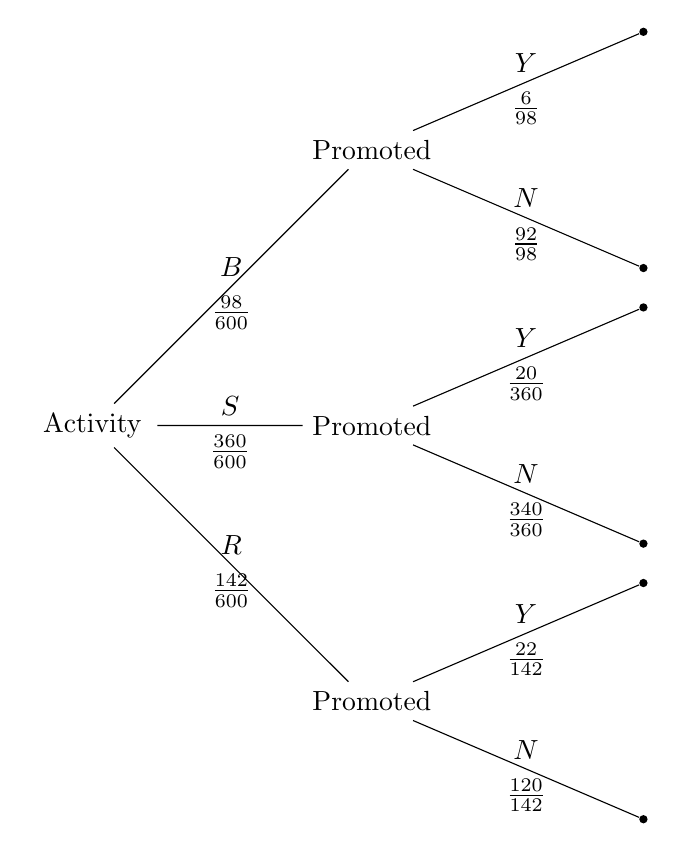
\begin{tikzpicture}[grow=right]
\node[bag] {Activity}
    child {
        node[bag] {Promoted}% This is the first of three "Bag 2"
        child {
                node[end] {}
                                edge from parent
                node[above] {$N$}
                node[below]  {$\frac{120}{142}$}
            }
            child {
                node[end] {}
                                edge from parent
                node[above] {$Y$}
                node[below]  {$\frac{22}{142}$}
            }
              edge from parent 
            node[above] {$R$}
            node[below]  {$\frac{142}{600}$}
    }
    child {
        node[bag] {Promoted}
            child {
                node[end] {}
                                          edge from parent 
                                node[above] {$N$}
                node[below]  {$\frac{340}{360}$}
            }
            child {
                node[end] {}
                                          edge from parent 
                                node[above] {$Y$}
                node[below]  {$\frac{20}{360}$}
            }
                          edge from parent 
            node[above] {$S$}
            node[below]  {$\frac{360}{600}$}
    }
    child {
        node[bag] {Promoted}
            child {
                node[end] {}
                                                          edge from parent 
                                                node[above] {$N$}
                node[below]  {$\frac{92}{98}$}
            }
            child {
                node[end] {}
                                          edge from parent 
                                                node[above] {$Y$}
                node[below]  {$\frac{6}{98}$}
            }
                    edge from parent         
            node[above] {$B$}
            node[below]  {$\frac{98}{600}$}
    };
\end{tikzpicture}
\end{center}

\begin{benumerate}
\item If an employee is selected at random, what is the probability that they attended the brainstorming session \underline{and} were promoted?

We are interested in finding $P(B \cap Y)$. Recall Bayes' Theorem,
\[ P(Y|B) = \frac{P(B \cap Y)}{P(B)}\]
Rearranging we find
\[ P(B \cap Y) = P(Y|B) \cdot P(B)\]
From our tree we know that $P(B) = \frac{98}{600} \approx 0.16$ and $P(Y|B) = \frac{6}{98} \approx 0.06$. Plugging these into our equation for $P(B \cap Y)$ yields
\[ P(B \cap Y) = P(Y|B) \cdot P(B) = 0.06 \cdot 0.16 \approx 0.01\]

\item If an employee is selected at random, what is the probability that they attended the skills workshop \underline{and} were promoted?

We are interested in $P(S \cap Y)$. From part (a) we know that
\[ P(S \cap Y) = P(Y|S) \cdot P(S) \]
From our tree we know that $P(S) \approx 0.6$ and $P(Y|S) \approx 0.06$. Plugging these into our equation for $P(S \cap Y)$ yields 
\[ P(S \cap Y) = P(Y|S) \cdot P(S) = 0.6 \cdot 0.06 \approx 0.04 \]
\end{benumerate}
\end{example}

\section{Counting Techniques}


\subsection{Factorial}
\index{Factorial}

The factorial is a a very useful function used in combinatorics.
The factorial of a non-negative integer $n$ is denoted
as $n!$ and it is the product of all positive integers less than or equal to $n$.

\begin{definition}[Factorial (!)]
Let $n$ be any non-negative integer. The factorial of $n$ is
	\setlength{\jot}{8pt}
	\begin{align}
	n! & = n \cdot (n - 1) \cdot (n - 2) \cdot \ldots \cdot 2 \cdot 1	\\
	0! & = 1
	\end{align} 
\end{definition}

The factorial is very useful in solving problems involving counting
the number of ways we can arrange a number of items. The number of ways that we can arrange $n$ items is $n!$ The reason that $0!= 1$ by definition is because there is only one way that we can arrange no items (and that is to not do anything). The reason for defining $0!= 1$ will also become more apparent when
we study combinations and permutations.



\subsection{Combinations}
\index{Combinations}

In counting problems we often would like to consider 
randomly drawing a sample of size $k$ from a population of size $n$.
The number of ways which we can achieve this is provided by
binomial coefficient and this value is calculated as follows.

\begin{definition}[Binomial Coefficient]
\label{definitionBinomialCoefficient}
\index{Binomial coefficient}
The number of ways which we can choose $k$ items out of a total of $n$ items such that order does not matter is 
		\begin{equation}
		{_{n}C_{k}} = {n \choose k} = \frac{ n! }{ k! (n - k)! }
		\end{equation}
\end{definition}

\noindent
Furthermore when we choose $k$ items, they are not distinct items.\\

\begin{example}
Suppose that the University of Guelph offers 23 courses that will satisfy business degree requirements but you can only choose 5 for the fall semester. How many different collections of 5 courses can you choose in the fall semester? \\

\hfill\\
{\emph{\textbf{\underline{Solution:}}}}\\


There are $_{23}C_{5}$ different collections of 5 fall semester courses.

\[ _{23}C_{5} = {23 \choose 5} = \frac{23!}{5!(23-5)!} = 33649 \]
\\
In the following winter semester how many choices will you have, assuming that you passed all of your courses in the fall semester?\\

Since we already passed 5 out of the 23 possible courses, we only have 18 left to choose from. Therefore, there are $_{18} C_{5}$ ways of selecting 5 winter semester courses.

\[ _{18} C_{5} = {18 \choose 5} = \frac{18!}{5!(23-5)!}=8569\]

\end{example}

\begin{example}
Use factorials or the binomial coefficient to solve the following.
\begin{benumerate}
\item How many ways can we arrange the numbers 0 through 9 if each number can only be selected once? \\
For the first number, we have 10 possibilities. Since we already selected the first number, we only have 9 possibilities for the second number. Since we already chose two numbers for the first and second number, we only have 8 possibilities for the third number, etc. Therefore, there are
\[10! =  10 \times 9 \times 8 \times 7 \times 6 \hdots \times 1 = 3,628,800\]
ways to arrange the numbers 0 through 9.


\item A standard license plate has 7 characters. If the characters can take on the values of 0-9, each number can only be used once, and each combination of numbers is unique, how many ways can we choose a license plate number? 

Since we are only choosing 7 characters, we have 10 choices for the first number, 9 choices for the second number, $\hdots~$, 4 choices for the seventh number. That is there are 
\[ 10 \times 9 \times 8 \times \hdots \times 4 = 604, 800 \]
ways to arrange seven numbers from 0 through 9. This is equivalent to 
\[ \frac{10!}{3!} = \frac{10 \times 9 \times 8 \times \hdots \times 1}{3 \times 2 \times 1} \]

\item If each combination of numbers on a license place is not unique, how many ways can we choose a license plate number? 

From part (a) and via the factorial, we know that the 7 numbers we select can be arranged $7!$ ways. But since order doesn't matter, we assume that all $7!$ ways are the same. That is to say, 1 2 3 4 5 6 7 is equivalent to 7 6 5 4 3 2 1, etc. Therefore, assuming order doesn't matter we can choose a license plate with the numbers 0 through 9
\[ \frac{10!}{3!7!} = 120 \]
different ways. This is $_{10}C_{7}$.

\end{benumerate}
\end{example}

\section{Random Variables}
\index{Random variables}

A random variable is the realization of what we previously called an experiment with a numerical outcome. The term might be a little misleading since a random variable is actually a function.We usually denote a random variable with a capital letter (such as $X$) and the values it takes with a lowercase letter (such as $x$).

\hfill
\begin{definition}[Random Variable]
\index{Random variables!Definition}
\label{definitionRandomVariable}
Let $\Omega$ be a sample space. 
A random variable (RV) $X$ is a function that maps events in
$\Omega$ to a real number.
	\begin{equation}
	X : \Omega \longrightarrow \mathbb{R}
	\end{equation}
\end{definition}


\begin{nt}
Definition $\ref{definitionRandomVariable}$ above is not completely correct but it is sufficient for the purposes of an introductory course in statistics.
We can consider a random variable to be a well defined map where every event in
the sample space is mapped to some number. 
The proper definition of a random variable involves a mathematical set of events known as a \textit{sigma algebra}
(or \textit{sigma field}) and is better suited for more advanced courses such as mathematical statistics,
mathematical analysis or measure theory.
\end{nt}

\subsection{Discrete Random Variables}
\label{sectionDiscreteRandomVariable}
\index{Random variables!Discrete}

\begin{definition}[Discrete Random Variables]
A discrete random variable is a random variable that can only take specific (i.e. discrete) values.
\end{definition}

\noindent
Using a \textit{probability distribution function}, we can assign probabilities to every possible value of a random variable.

\subsubsection{Probability Mass Function}
\index{Probability!Mass function}


The \textit{probability distribution function} of a discrete random variable is called a 
\textit{probability mass function} (PMF) 
or mass function for short.
If $X$ is a discrete random variable with outcomes $x = x_{1},~x_{2},~\ldots~$, the probability that $X$ takes on a specific value $x_i$ is $P(X = x_{i})$ or simply  $p(x_{i})$.

\begin{properties}
Let $X$ be a discrete random variable with possible values $x = x_{1},~x_{2},~\ldots$ The probability mass function of $X$ consists of individual probabilities $p(x_i)$ with the following properties:
	\begin{enumerate}
	\item	$0 \leq p(x_{i}) \leq 1$ \\[0.5em]
	\item	$\displaystyle\sum_{\forall i} p(x_{i}) = 1 $
	\end{enumerate}
\end{properties}

\noindent
Note that we are being general in terms of the full range of $X$ because it can be finite or infinite (This is why we have written $\forall i$ and not $i = 1,2, \ldots, n$).\\

\noindent
A probability mass function can be expressed in tabular form for convenience. For a discrete random variable $X$ with possible values $x_1,~x_2,~\hdots~,~x_n$,

\begin{table}[h]
\begin{center}
\begin{tabular}{c|c|c|c|c}
\def\arraystretch{1.5}
$X=x$	&	$x_{1}$	&	$x_{2}$	&	\ldots	&	$x_{n}$	\\
\hline
$P(X=x)$	&	$p(x_{1})$	&	$p(x_{2})$	&	\ldots	&	$p(x_{n})$	\\
\end{tabular}
\caption{Probability mass function of discrete random variable $X$.}
\end{center}
\end{table}

\subsubsection{Mean, Variance and Standard Deviation of a Discrete Random Variable}

\begin{definition}[Mean of a Discrete Random Variable]
Let $X$ be a discrete random variable with outcomes $x_{1}$, \ldots, $x_{n}$
which have corresponding probabilities $P(X = x_{1})$, \ldots, $P(X = x_{n})$.
The mean of $X$ is the sum of each outcome $x_{i}$ multiplied by their corresponding probability $P(X=x_{i})$:
%Let $X$ be a discrete random variable.
%The mean of $X$ is given by.
\begin{align}
\mu = \mathbb{E}(X) & = \displaystyle\sum_{\forall i} x_{i} \cdot p(x_{i}) \\
				& = x_{1} \cdot p(x_{1}) + x_{2} \cdot p(x_{2}) + \ldots
\end{align}
\end{definition}


This mean is the population mean  and not the sample mean.
The population mean is also referred to as the \textit{expected value}, denoted by 
$\mathbb{E}(x)$. 

\begin{definition}[Variance \& Standard Deviation of a Discrete RV]
Let $X$ be a discrete random variable with outcomes $x_{1}$, \ldots, $x_{n}$
which have corresponding probabilities $P(X = x_{1})$, \ldots, $P(X = x_{n})$
and mean $\mu = \mathbb{E}(X)$.
The variance of $X$ is calculated as
\begin{align}
\sigma^{2}	 & = \mathbb{E} \big( (X - \mu)^{2} \big)\\
		 & = \displaystyle\sum_{\forall i} (x_{i} - \mu)^{2} \cdot p(x_{i}) \\
		& = (x_{1} - \mu)^{2} \cdot p(x_{1}) + (x_{2} - \mu)^{2} \cdot p(x_{2}) + \ldots
\end{align}
\noindent
and the standard deviation of $X$ is 
\begin{align}
\sigma	& = + \sqrt{ \sigma^{2} }
\end{align}
\end{definition}

\hfill
\begin{nt}
An alternative (and sometimes easier) way to calculate the variance of a discrete random variable is:
\begin{align}
\sigma^{2}		& = \mathbb{E}(X^{2}) - \big( \mathbb{E}(X) \big)^{2}	\\
			& = \bigg(\displaystyle\sum_{\forall i}  x^{2} \cdot p(x_{i})  \bigg) - \mu^{2} \\
			& = \bigg( x_{1}^{2} \cdot p(x_{1}) + x_{2}^{2} \cdot p(x_{2}) + \ldots \bigg) - \mu^{2}
\end{align}
\end{nt}

\begin{example}
Consider the following probability mass function for random variable $X$.

\begin{center}
\begin{tabular}{c|c|c|c|c|c|c|c|c}
\def\arraystretch{1.5}
$X=x$ & 1 & 2 & 3 & 4 & 5 & 6 & 7 & 8 \\ 
\hline 
$P(X=x)$ & 0.05 & 0.02 & 0.07 & 0.36 & 0.33 & 0.06 & 0.05 & 0.06 \\ 
\end{tabular} 

\begin{benumerate}
\item Is this a proper probability mass function?\\

In order to determine if this is a proper probability mass function, we need to make sure the following two properties hold.
\begin{enumerate}[1.]
\item $0 \leq p(x_i) \leq 1$.
\item $\sum_{i=1}^{8} p(x_i) = 1$.
\end{enumerate}

Through observation of the table, it is clear that $0 \leq p(x_1), \hdots , p(x_8) \leq 1$ and
\[ \sum_{i=1}^{8} p(x_i) = 0.05 + 0.02 + \hdots + 0.06 = 1 \] 
Both properties hold and therefore this is a proper probability mass function.

\item	Sketch the mass function for $X$.
\item[]	\begin{center}
		\frame{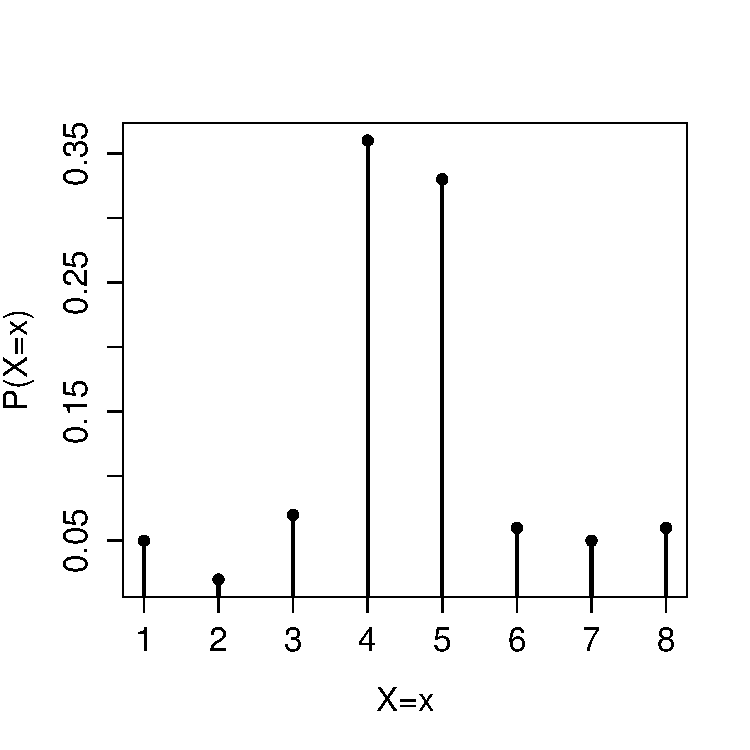
\includegraphics[scale=0.5]{Section3/examplepmf.pdf}}
		\end{center}


\item Find the mean of $X$.
\begin{align*}
\mu = \mathbb{E}(X) &= \sum_{i=1}^{8} x_i \cdot p(x_i) \\
	&= 0.05 \times 1 + 0.02 \times 2 + 0.07 \times 3 + \hdots + 0.05 \times 7 + 0.06 \times 8 \\
	&= 4.58
\end{align*}

\item Find the variance of $X$.
\begin{align*}
\sigma^2 &= \mathbb{E} \bigg( (X-\mu)^2 \bigg) \\
		 &= \sum_{i=1}^{8} (x_i - \mu)^2 \cdot p(x_i) \\
		 &= (1-4.58)^2 \times 0.05 + (2-4.58)^2 \times 0.02 + (3 - 4.58)^2 \times 0.07 \\
		 &+ \hdots + (7-4.58)^2 \times 0.05 + (8-4.58)^2 \times 0.06 \\
		 &= 0.6408 + 0.1331 + 0.1747 + \hdots + 0.2928 + 0.7018 \\
		 &= 2.2436
\end{align*}

Alternatively,
\begin{align*}
\sigma^{2} = E(X^2) - \bigg( E(X) \bigg) ^2 
\end{align*}
From part (b), we know $E(X)=4.58$ and therefore $\bigg(E(X)\bigg)^2 = 4.58^2 = 20.9764$.

\begin{align*}
E(X^2) 	&= \sum_{i=1}^{8} x_i^2 \cdot p(x_i) \\
		&= 1^2 \times 0.05 + 2^2 \times 0.05 + 3^2 \times 0.05 + \hdots + 7^2 \times 0.05 + 8^2 \times 0.06 \\
		&= 0.05 + 0.08 + 0.63 + 5.76 + 8.25 + 2.16 + 2.45  + 3.84 \\
		&= 23.22 \\
\Rightarrow \sigma^2 &= 23.22 - 20.9764 = 2.2436 \text{~ as before.}
\end{align*}
\item Find the standard deviation of $X$.
\[ \sigma = +\sqrt{\sigma^{2}} = \sqrt{2.2436} = 1.498 \]

\end{benumerate}

\end{center}

\end{example}

\begin{example}
Consider the following probability mass function.

\begin{center}
\begin{tabular}{c|c|c|c|c|c}

X=x & -2 & -1 & 0 & 1 & 2 \\ 
\hline 
P(X=x) & 0.3 & 0.2 & $a$ & 0.1 & 0.15 
 
\end{tabular} 
\end{center}

\begin{benumerate}
\item What is $a$?
In order to be a valid probability mass function,
\[ \sum_{\forall i} p(x_i) = 1 \]
Therefore we know that
\[ 0.3 + 0.2 + a+ 0.1 + 0.15 = 1 \]
Rearranging for $a$ we find
\[ a = 1-0.75 = 0.25 \]

\item Find $\mu$.
\begin{align*}
\mu = \sum_{\forall i} x_i \cdot p(x_i)  = (-2)(0.3) + (-1)(0.2) + 0 + (1)(0.1)+(2)(0.15) = -0.40
\end{align*}
\item Find $\sigma^{2}$.
\begin{align*}
\sigma^{2} &= E(X^2) - \Big( E(X) \Big)^2
\end{align*}
\begin{align*}
E(X^2) = \sum_{\forall i} x_i^2 \cdot p(x_i) = (-2)^2 (0.3) + (-1)^2(0.2) + \hdots + (2)^2(0.15) = 2.1
\end{align*}
\begin{align*}
\sigma^{2} = 2.1 - (-0.40)^2 = 1.94
\end{align*}
\end{benumerate}
\end{example}

\subsection{Continuous Random Variable}
\index{Random variables!Continuous}

A continuous random variable is a random variable that can take any value within
a specified range. 
The support of a continuous variable has infinite precision
meaning that we can make our measurement as
fine as we would like. 

\subsubsection{Probability Density Function}
\index{Probability!Density function}

Recall that in
Section $\ref{sectionDiscreteRandomVariable}$ a discrete random variable was associated with a probability mass function.
We associate continuous random variables with a \textit{probability density function} (PDF) or density function for short. \\

When we sketched the probability mass function, we got point masses at the values of the random variable. With continuous random variables, the density function is a continuous curve where the domain is the support of the random variable.


\begin{properties}
Let $X$ be a continuous random variable with support $[\alpha, \beta]$.\\	
We say that $f(x)$ is the probability distribution function of $X$ if it satisfies the following properties:\\
	\begin{enumerate}
	\item	$f(x) \geq 0,\quad \forall x \in [\alpha,\beta]$\\[0.5em]
	\item	$P(a \leq x \leq b) = \displaystyle\int_a^b f(x) \,dx$ \\[0.5em]
	\item $\displaystyle\int_{-\infty}^{+\infty} f(x) \,dx = 1 $\\[0.5em]
	\item	$P( x = c) = 0, \quad \forall c \in \mathbb{R}$
	\end{enumerate}
\end{properties}

If the reader is familiar with calculus, recall that that the definite integral of a function $f(x)$ from limits $a$ to $b$ gives the area between the curve and the $x$-axis.
With a density function the area under the curve gives us the probability.
A deeper understanding of density functions requires a proper knowledge of integral calculus.
For this introductory course a knowledge of calculus is not required however we will provide the definition of the mean and variance of a continuous random variable for completeness.

\subsubsection{Mean, Variance and Standard deviation of a Continuous Random Variable}


\begin{definition}[Mean of a Continuous Random Variable]
Let $X$ be a continuous random variable with density function $f(x)$. 
The mean of $X$ is given by:
\begin{align}
\mu = \mathbb{E}(X) = \displaystyle\int_{- \infty}^{+ \infty} x \cdot f(x) \, dx
\end{align}
\end{definition}

\begin{definition}[Variance and Standard Deviation of a Continuous RV]
Let $X$ be a continuous random variable with density function $f(x)$. 
The variance of $X$ is calculated as
\begin{align}
Var(X) = \sigma^{2} 	& = \mathbb{E}[ \big(X - \mathbb{E}(X) \big)^2 ] \\
				& = \int^{+ \infty}_{- \infty} (x - \mu)^{2} \cdot f(x) \, dx
				%& = \mathbb{E}(X^{2}) - \big( \mathbb{E}(X) \big)^{2}
\end{align}
\noindent
and the standard deviation of $X$ is 
\begin{align}
\sigma	& = + \sqrt{ \sigma^{2} }
\end{align}
\end{definition}

\begin{example}
Suppose $X$ is a continuous random variable with support $[0,1]$. 
\begin{benumerate}
\item Is $f(x) = 3x^2$ a valid pdf for $X$?

\begin{align*}
\int_{-\infty}^{+\infty} f(x) dx &= \int_{0}^{1} 3x^2dx 
	= \frac{3x^3}{3} \bigg|_{x=0}^{x=1} 
	= 1^{3} - 0^{3} = 1
\end{align*}

This is a valid pdf.

\item What is the mean of $X$?
\begin{align*}
\mu = \mathbb{E}(X) &= \int_{0}^{1} x \times 3 x^2 dx 
			  = \int_{0}^{1} 3 x^{3} dx 
			  = \frac{3 x^{4}}{4} \bigg|_{x=0}^{x=1}
			  = \frac{3}{4}(1^4) - \frac{3}{4}(0^4) = \frac{3}{4}
\end{align*}

\item What is the variance of $X$?
\begin{align*}
\mathbb{E}(X^2) &= \int_{0}^{1} x^2 \times 3 x^2 dx 
				= \frac{3x^5}{5} \bigg|_{x=0}^{x=1}
				= \frac{3}{5}\\
\Rightarrow Var(X) &= \mathbb{E}(X^2) - \bigg( E(X) \bigg)^2 
= \frac{3}{5} - \left( \frac{3}{4} \right)^2 = \frac{3}{80}
\end{align*}
\item What is $P(X \geq 0.5)$?
\begin{align*}
P(X \geq 0.5) &= \int_{0.5}^{1} 3x^2 dx 
			= x^3 \bigg|_{x=0.5}^{x=1} 
			= 1 - 0.5^3 
			= 0.875
\end{align*}
\end{benumerate}
\end{example}








%\pagebreak
%
%\section{Basic Definitions}
%
%\subsection{Preliminaries}
%
%%\begin{frame}[<+->] \frametitle{Preliminaries} \pause
%
%An \textbf{experiment} is the occurrence of an observation that is not predictable.  We will use
%this definition for now but we will call it something else next week. %\pause
%
%\smallskip
%
%A \textbf{sample point} is the basic realization of an experiment. %\pause
%
%\smallskip
%
%The \textbf{sample space} is the collection of all sample points.%\pause
%
%\smallskip
%
%We attach a \textbf{probability} to each sample point, $p_i$, say for $i=1,\dots ,n$ sample points
%and we insist that %\pause
%\begin{itemize}
%\item $0 \leq p_i \leq 1$ for all $i=1,\dots ,n$
%\item $\sum_{i=1}^np_i = 1$
%\end{itemize}
%
%
%%\iffalse %\fi line 147
%%
%%\begin{frame}
%%
%%\vspace{-.4 cm}
%%\includegraphics[width=11.5cm]{phew}
%%
%%\end{frame}
%%
%%\begin{frame}[<+->] \frametitle{Again} \pause
%%
%%An \alert{experiment} is the occurrence of an observation that is not predictable.  We will use
%%this definition for now but we will call it something else next week. \pause
%%
%%\smallskip
%%
%%A \alert{sample point} is the basic realization of an experiment. \pause
%%
%%\smallskip
%%
%%The \alert{sample space} is the collection of all sample points.\pause
%%
%%\smallskip
%%
%%We attach a \alert{probability} to each sample point, $p_i$, say for $i=1,\dots ,n$ sample points
%%and we insist that \pause
%%\begin{itemize}
%%\item $0 \leq p_i \leq 1$ for all $i=1,\dots ,n$
%%\item $\sum_{i=1}^np_i = 1$
%%\end{itemize}
%%
%%\end{frame}
%%
%%\begin{frame}[<+->] \frametitle{One more time} \pause
%%
%%An \alert{experiment} is the occurrence of an observation that is not predictable.  We will use
%%this definition for now but we will call it something else next week. \pause
%%
%%\smallskip
%%
%%A \alert{sample point} is the basic realization of an experiment. \pause
%%
%%\smallskip
%%
%%The \alert{sample space} is the collection of all sample points.\pause
%%
%%\smallskip
%%
%%We attach a \alert{probability} to each sample point, $p_i$, say for $i=1,\dots ,n$ sample points
%%and we insist that \pause
%%\begin{itemize}
%%\item $0 \leq p_i \leq 1$ for all $i=1,\dots ,n$
%%\item $\sum_{i=1}^np_i = 1$
%%\end{itemize}
%%
%%\end{frame}
%%
%%\fi
%
%
%
%%Will  be given in class.
%
%
%
%
%%\begin{frame}[<+->] \frametitle{Events}
%
%An \textbf{event} is a collection of sample point(s). % \pause
%
%\smallskip
%
%They are distinguished by a \textbf{simple event}, which consists only of one
%sample point,  %\pause
%
%\smallskip
%
%as opposed to more than one sample point called a \textbf{compound event}.  %\pause
%
%\smallskip
%
%If we denote some event, either simple or compound, then the \textbf{probability of an event} is determined by adding the
%probabilities for each of the sample point(s) in the event.
%
%
%
%Will  be given in class.
%
%%\end{frame}
%
%%\begin{frame}[<+->] \frametitle{Diagrams}
%
%Two very effective ways of illustrating these concepts is through what are called
%
%\begin{itemize}
%
%\item[1.] \textbf{trees}
%
%\item[2.] \textbf{Venn diagrams}
%
%\end{itemize} %\pause
%
%Both are abstractions of these concepts that provide details (in different ways) of what  underlies the problem.
%
%%\end{frame}
%
%%\begin{frame}[<+->] \frametitle{Examples}
%
%Will  be given in class.
%
%%\end{frame}
%\iffalse
\documentclass[12pt]{article}
\usepackage{amsmath}
\usepackage{latexsym}

\addtolength{\textwidth}{1in} \addtolength{\oddsidemargin}{-0.5in}
\addtolength{\textheight}{1.6in} \addtolength{\topmargin}{-0.8in}

\newfont{\tebbb}{msbm10 scaled\magstep1}

\newtheorem{theorem}{Theorem}[section]
\newtheorem{proposition}[theorem]{Proposition}
\newtheorem{lemma}[theorem]{Lemma}
\newtheorem{corollary}[theorem]{Corollary}
\newtheorem{remark}[theorem]{Remark}
\newtheorem{example}[theorem]{Example}
\newcommand{\beq}{\begin{equation}}
\newcommand{\eeq}{\end{equation}}
\newtheorem{definition}[theorem]{Definition}


\newcommand{\cross}[2]{{{\bf{#1}} \times {\bf{#2}}}}
\newcommand{\dotprod}[2]{{{\bf{#1}} \cdot {\bf{#2}}}}
\newcommand{\real}[1]{{\mbox{\tebbb R}}^{#1}}
\newcommand{\norm}[1]{\|{\bf{#1}}\|}
\renewcommand{\theequation}{\thesection.\arabic{equation}}

\baselineskip = 20pt plus 3pt minus 3pt

\begin{document}
\fi
\section{Suggested Exercises}\label{ssec.se3}\markright{\ref{ssec.se3} \titleref{ssec.se3}}
\begin{enumerate}
\item Which hypothesis,the null or the alternative,is the statusquo hypothesis?Which is the research hypothesis?
\item What is a test statistics?
\item Define $\alpha$ and  $\beta$. How do they relate to Type I and Type II errors?
\item If you test a hypothesis and reject the null hypothesis in favor of the alternative hypothesis,does your test prove that the alternative hypothesis is correct?Explain.
\item List all possible results of the combinations of decisions and true states of nature ofr a test of hypothesis.
\end{enumerate}

\iffalse
\begin{enumerate}
\item  Let $A=\left[
\begin{array}{rr}
2 & 3 \\ 3 & 5 \end{array} \right ]$ and calculate:
\begin{enumerate}
\item $A^{-1}$
\item (i) $4A$ \quad (ii) $(4A)^{-1}$
\item (i) $A^t$ \quad (ii) $(A^t)^{-1}$
\item (i) $A^3$ \quad (ii) $A^{-3}.$
\end{enumerate}
\item Let $B= \left[
{\begin{array}{rr}
2 & 5 \\
1 & 3
\end{array}}
 \right]$ and $A$ as above. Find
\begin{enumerate}
\item $B^{-1}$
\item (i) $AB$ \quad (ii) $(AB)^{-1}$ \quad (iii) $B^{-1}A^{-1}$
\end{enumerate}
\item For each of the following calculate the inverse.
\begin{enumerate}
\item $\left[ {\begin{array}{rrr} 1 & 0 & 2 \\ 2 & -1 & 3 \\ 4 & 1 &
8
\end{array}}
 \right]$
\item $\left[ {\begin{array}{rrr} 1 & 2 & 1 \\ 1 & 1 & 1 \\ 3 & -1 &
1
\end{array}}
 \right]$
\item $ \left[ {\begin{array}{rrr} 1 & 3 & -4 \\ 1 & 5 & -1 \\ 3 &
13 & -6
\end{array}}
 \right]
$
\item $\left[ {\begin{array}{rrr} 0 & 1 & 1 \\ 5 & 1 & -1 \\ 2 & -3
& -3
\end{array}}
 \right]$
\item $\left [\begin {array}{rrrr} 1&0&0&0\\2&-2&0&0
\\3&1&-2&0\\1&-1&3&0\end {array}
\right ]$
\item $ \left[ {\begin{array}{rrrr} 1 & 2 & 1 & 0 \\ 0 &
1 & -1 & 0 \\ 1 & 3 & 1 & -2 \\ 1 & 4 & -2 & 4
\end{array}}
\right]$
\end{enumerate}
\item Solve the following system using matrix inversion.
\begin{eqnarray*} x_1+2x_2+x_3&=&1\\
x_2-x_3&=&-1\\ x_1+3x_2+x_3-2x_4&=&-2\\ x_1+4x_2-2x_3+4x_4&=&4
\end{eqnarray*}
\item Let $A= \left[
\begin{array}{rr}
1 & 5 \\
0 & 1
\end{array}
 \right]$, $B= \left[
\begin{array}{rr}
2 & 3 \\
1 & -2
\end{array}
 \right]$ $C= \left[
\begin{array}{rr}
3 & -5 \\
-1 & 2
\end{array}
 \right]$
 $D= \left[
\begin{array}{rr}
-3 & -5 \\
7 & 2
\end{array}
 \right]$  find
\begin{enumerate}
 \item (i) $\det(A)$ \quad (ii) $\det(B)$ \quad (iii) $\det(C)$ \quad (iv) $\det(D)$
 \item (i) $\det(A+B)$ \quad (ii) $\det(A)+\det(B)$
 \item (i) $\det(3A)$ \quad (ii) $\det(B^t)$
 \item (i) $AB$ \quad (ii) $\det(AB)$ \quad (iii) $\det(A)\det(B)$
 \item $\det(D^{-1})$
\end{enumerate}
\item Let $G=\left[
{\begin{array}{rrr}
1 & 0 & 1 \\
2 & 3 & 1 \\
-7 & 0 & -7
\end{array}}
 \right]$,
$H =  \left[
{\begin{array}{rrr}
1 & 2 & 3 \\
4 & 6 & 5 \\
3 & 2 & 7
\end{array}}
 \right]$,
$J =  \left[
{\begin{array}{rrr}
-2 & 4 & -6 \\
3 & -5 & 7 \\
9 & -6 & -3
\end{array}}
 \right]$ find
\begin{enumerate}
\item (i) $\det(G)$ \quad (ii) $\det(G^t)$ \quad
\item $\det(H)$
\item $\det(J)$
\item (i) $\det(HJ)$ (ii) $\det(GJ)$
\end{enumerate}
\item Find $\det(A)$ and $\det(A^{-1})$ for
\begin{align*}
\mathrm{(a)}\ \ A &= \left[ \begin{array}{rrrr} 1 & 2 & 1 & 0 \\ 0 & 1 & -1 & 0
\\ 1 & 3 & 1 & -2 \\ 1 & 4 & -2 & 4 \end{array} \right]&
\mathrm{(b)}\ \ A&= \left[ {\begin{array}{rrrr} 10 & -3 & -3 & -2 \\ 10 & -3 &
-4 & -3 \\ -6 & 2 & 2 & 1 \\ -3 & 1 & 1 & 1 \end{array}} \right]
\end{align*}

\item We have seen that systems of equations can be solved  using either
Gaussian elimination or with ${\bf x}=A^{-1}{\bf b}$. Determine
which of the two methods are appropriate for the following two
systems.
\begin{align*}
\mathrm{(a)}\qquad \quad \quad \ x_1-x_3&=-1& \mathrm{(b)}\ \ 2x_1+x_2-x_3&=6\\
11x_1+2x_2+x_3&=2& 3x_1-x_2&=1\\
3x_1+x_2+3x_3&=1& 9x_2+2x_3&=0
\end{align*}

\end{enumerate}

\section{Answers to activity questions and suggested exercises}
\label{answers3}\markright{\ref{answers3}
\titleref{answers3}}

{\bf Activity questions}

\bigskip

\noindent {\bf \ref{ssec.definv}:}
\begin{enumerate}
\item (a), but not (b).
\item $I$.
\end{enumerate}

\bigskip

\noindent {\bf \ref{ssec.findinv}:}

\begin{enumerate}
\item \begin{enumerate}
\item
\begin{eqnarray*}
& &
\left[ \begin{array}{rrrcrrr} 1 & 0 & 1 & \vline & 1 & 0 & 0\\
                             -1 & 1 & 2 & \vline & 0 & 1 & 0\\
                              2 & 2 & 9 & \vline & 0 & 0 & 1
\end{array} \right]
\\&&\hspace{-12mm}
\overset{\begin{smallmatrix}R_2+R_1\\R_3-2R_1\end{smallmatrix}}{\leadsto}
\left[ \begin{array}{rrrcrrr} 1 & 0 & 1 & \vline & 1 & 0 & 0\\
                              0 & 1 & 3 & \vline & 1 & 1 & 0\\
                              0 & 2 & 7 & \vline & -2 & 0 & 1
\end{array} \right]
\\&&\hspace{-11mm}
\overset{R_3-2R_2}{\leadsto}
\left[ \begin{array}{rrrcrrr} 1 & 0 & 1 & \vline & 1 & 0 & 0\\
                               0 & 1 & 3 & \vline & 1 & 1 & 0\\
                               0 & 0 & 1 & \vline & -4 & -2 & 1
\end{array} \right]
\\&&\hspace{-12mm}
\overset{\begin{smallmatrix}R_1-R_3\\R_2-3R_3\end{smallmatrix}}{\leadsto}
\left[\begin{array}{rrrcrrr} 1 & 0 & 0 & \vline & 5 & 2 & -1\\
                               0 & 1 & 0 & \vline & 13 & 7 & -3\\
                               0 & 0 & 1 & \vline & -4 & -2 & 1
\end{array} \right].
\end{eqnarray*}
The inverse is
$\left[ \begin{array}{rrr} 5&2&-1\\13&7&-3\\-4&-2&1 \end{array} \right]$.
\item
\begin{eqnarray*}&&
\left[ \begin{array}{rrrcrrr} 1 & 0 & 1 & \vline & 1 & 0 & 0\\
                               1 & 1 & 0 & \vline & 0 & 1 & 0\\
                               -1 & 1 & -2 & \vline & 0 & 0 & 1
\end{array} \right]\\
 \overset{\begin{smallmatrix}R_2-R_1\\R_3+R_1\end{smallmatrix}}{\leadsto}
&&\vspace{-10mm}\left[ \begin{array}{rrrcrrr} 1 & 0 & 1 & \vline & 1 & 0 & 0\\
                              0 & 1 & -1 & \vline & -1 & 1 & 0\\
                              0 & 1 & -1 & \vline & -1 & 0 & 1
\end{array} \right]\\ \\
\overset{R_3-R_2}{\leadsto}
&&\vspace{-10mm}\left[ \begin{array}{rrrcrrr} 1 & 0 & 1 & \vline & 1 & 0 & 0\\
                               0 & 1 & -1 & \vline & -1 & 1 & 0\\
                               0 & 0 & 0 & \vline & 0 & -1 & 1
\end{array} \right].
\end{eqnarray*}
The matrix does not reduce to $I$ so $\exists$ no inverse.
\item
\begin{eqnarray*}
&&
\left[ \begin{array}{rrrrcrrrr}  1 & 0 & 0 & 0 & \vline & 1 & 0 & 0 & 0\\
                                 0 & 0 & 0 & 1 & \vline & 0 & 1 & 0 & 0\\
                                 0 & 0 & 1 & 0 & \vline & 0 & 0 & 1 & 0\\
                                 0 & 1 & 0 & 0 & \vline & 0 & 0 & 0 & 1
\end{array} \right] \\ \\\overset{R_2\leftrightarrow R_4}{\leadsto}
&&\vspace{-10mm}\left[ \begin{array}{rrrrcrrrr}  1 & 0 & 0 & 0 & \vline & 1 & 0 & 0 & 0\\
                                 0 & 1 & 0 & 0 & \vline & 0 & 0 & 0 & 1\\
                                 0 & 0 & 1 & 0 & \vline & 0 & 0 & 1 & 0\\
                                 0 & 0 & 0 & 1 & \vline & 0 & 1 & 0 & 0
\end{array} \right].
\end{eqnarray*}
 Hence this matrix is it's own inverse.

\end{enumerate}
\end{enumerate}

\bigskip

\noindent {\bf \ref{ssec.propinv}:}\\
\vspace{0.1\baselineskip}

\noindent {\bf Hints: } To prove number 5, what does
$(A^{-1})(A^{-1})^{-1}$ equal?  To prove number 7, use the exact
same method shown in the notes, except that you now multiply
$(kA)(\frac{1}{k}A^{-1}$).

\bigskip

\noindent {\bf \ref{ssec.syseinv}:}
\begin{enumerate}
\item $A^{-1}=\left [ \begin{array}{rrr}\vspace{1mm}
                                1&0&1\\ \vspace{1mm}
                                1&1&\frac{5}{2}\\
                                0&0&-\frac{1}{2} \end{array} \right
                                ]$,\  $x_1=\left [ \begin{array}{r}\vspace{1mm}
                                -2\\ \vspace{1mm}-\frac{5}{2}\\ \frac{3}{2}
                                \end{array} \right ]$,\ $x_2=\left [ \begin{array}{r} \vspace{1mm}
                                -11\\ \vspace{1mm} -\frac{13}{2}\\ \frac{1}{2}
                                \end{array} \right ]$.
\item Same as 1.

\item ${\bf x}={\bf 0}$.

\item If any other {\bf b} are introduced into the problem, by
theorem \ref{eq2invert} we know that the system will be consistent
and have exactly one solution for every {\bf b}.
\end{enumerate}

\noindent {\bf \ref{sec.det}:}
\begin{enumerate}
\item \begin{itemize} \item[(i)]
\begin{itemize}
\item[(a)] $2\left| \begin{array}{rr}2&-2\\0&1\end{array} \right| +
\left| \begin{array}{rr}3&-2\\0&1\end{array} \right| +
3 \left| \begin{array}{rr}3&2\\0&0\end{array} \right| = 4+3+0 = 7$
\item[(b)] $1\left| \begin{array}{rr}3&-2\\0&1\end{array} \right| +
2\left| \begin{array}{rr}2&3\\0&1\end{array} \right| +
0\left| \begin{array}{rr}2&3\\3&-2\end{array} \right| = 3+4+0 = 7$
\end{itemize}
\item[(ii)]
\begin{itemize}
\item[(a)] $2\left| \begin{array}{rr}1&2\\8&3\end{array} \right| -
3\left| \begin{array}{rr}0&2\\0&3\end{array} \right| +
2\left| \begin{array}{rr}0&1\\0&8\end{array} \right| = -26+0+0 = -26$
% START HERE
\item[(b)] $-3\left| \begin{array}{rr}0&2\\0&3\end{array} \right| +
1\left| \begin{array}{rr}2&2\\0&3\end{array} \right| -
8\left| \begin{array}{rr}2&2\\0&2\end{array} \right| = 0+6-32 = -26$
\end{itemize}
\end{itemize}
\item Expand matrix (i) along the bottom row
$$
\left| \begin{array}{rr}2&-1\\3&2\end{array}\right|
$$
Expand matrix (ii) along the bottom row
$$
2 \left| \begin{array}{rr}1&2\\8&3\end{array} \right| = 2(3-16) = -26
$$
\end{enumerate}

\noindent {\bf \ref{ssec.propdet}:}
\begin{enumerate}
\item
\begin{enumerate}
\item
$$
\begin{vmatrix}2&2&1\\2&1&1\\1&2&1\end{vmatrix} \overset{R_1 - R_3}{\leadsto}
\begin{vmatrix}1&0&0\\2&1&1\\1&2&1\end{vmatrix} = \begin{vmatrix}1&1\\2&1\end{vmatrix} = 1-2 =-1
$$
\item
\begin{eqnarray*}
\left| \begin{array}{rrrr} 1&2&7&5\\2&1&3&10\\4&-1&-3&20\\8&3&9&39
\end{array} \right|
&& \hspace{-5mm}\overset{\begin{smallmatrix}C_4 -
5C_1\\C_3-3C_2\end{smallmatrix}}{\leadsto} \quad \left|
\begin{array}{rrrr} 1&2&1&0\\2&1&0&0\\4&-1&0&0\\8&3&0&-1
\end{array} \right|\\
&=&
- \left| \begin{array}{rrr} 1&2&1\\2&1&0\\4&-1&0\end{array} \right| \\
&=& - \left| \begin{array}{rr}2&1\\4&-1\end{array} \right| \\&=&
-(-2-4) = 6
\end{eqnarray*}
\end{enumerate}
\item
\begin{enumerate}
\item -3
\item 270
\item -60
\item Not enough information
\end{enumerate}
\end{enumerate}
\noindent {\bf \ref{ssec.adjoint}:}  $A$ is invertible, since
det($A$)=17;  det($A^{-1}$)$=\frac{1}{17}$.


\bigskip

\noindent {\bf Suggested Exercises}

\begin{enumerate}
\item
\begin{enumerate}\item$ \left[ {\begin{array}{rr}5&-3\\-3&2 \end{array}}
\right]$\\
\item(i) $\left[ {\begin{array}{rr}8&12\\12&20\end{array}}
 \right]$\quad
(ii) $\left[ {\begin{array}{rr} \frac {5}{4}  & -\frac {3}{4}\\ -\frac {3}{4}  & \frac {1}{2}
\end{array}} \right]$
\item (i) $\left[ {\begin{array}{rr} 2 & 3 \\ 3 & 5 \end{array}}
\right]$ \quad (ii) $\left[ {\begin{array}{rr} 5 & -3 \\ -3 &
2\end{array}} \right]$
\item (i) $\left[ {\begin{array}{rr} 89 &
144
\\ 144 & 233
\end{array}}
 \right]$\quad
(ii) $
 \left[
{\begin{array}{rr}
233 & -144 \\
-144 & 89
\end{array}}
 \right]$
 \end{enumerate}

\item \begin{enumerate}
\item $ \left[
\begin{array}{rr}
3 & -5 \\
-1 & 2
\end{array}
 \right]$\\
\item (i) $\left[ {\begin{array}{rr} 7 & 19 \\ 11 & 30
\end{array}}
 \right]$ \quad (ii) $ \left[
{\begin{array}{rr}
30 & -19 \\
-11 & 7
\end{array}}
 \right]$ \quad (iii) $ \left[ {\begin{array}{rr} 30 & -19 \\ -11 & 7
\end{array}}
 \right]$
 \end{enumerate}
\item \begin{enumerate}
\item $ \left[ {\begin{array}{rrr} -11 & 2 & 2 \\ -4 & 0 & 1 \\ 6 &
-1 & -1
\end{array}}
 \right]
$
\item $\left[ {\begin{array}{rrr}\vspace{1mm} 1 & -\frac {3}{2}& \frac {1}{2}\\ \vspace{1mm}
1 & -1 & 0 \\ -2 & \frac {7}{2}  & -\frac {1}{2}
\end{array}}
 \right]$
\item Not Possible Singular matrix
\item $\left[ {\begin{array}{rrr}\vspace{1mm} \frac {3}{2} & 0 & \frac
{1}{2}\\ \vspace{1mm} -\frac {13}{4}  & \frac {1}{2} & -\frac {5}{4}  \\ \frac
{17}{4} & -\frac {1}{2} & \frac {5}{4}
\end{array}}
 \right]$
\item Not Possible \item $\left[ {\begin{array}{rccc} 10 & 10 & -6 &
-3
\\ -3 & -3 & 2 & 1 \\  -3 & -4  &
2& 1 \\-1 & -\frac{3}{2} & \frac{1}{2} & \frac{1}{2}
\end{array}}
\right]$
\end{enumerate}
\item $x_1=0,\ x_2=0,\ x_3=1,\ x_4=\tfrac{3}{2}$
\item
\begin{enumerate}
\item (i) 1 (ii) -7 (iii) 1 (iv) 29
\item (i) -11 (ii) -6
\item (i) 9 (ii) -7
\item (i) $ \begin{vmatrix} 7 & -7 \\1 & -2 \end{vmatrix}$ (ii) -7 (iii) -7
\item $\tfrac{1}{29}$
\end{enumerate}
\item
\begin{enumerate}
\item (i) 0 (ii) 0
\item -24
\item 12
\end{enumerate}
\item
\begin{enumerate}
\item (i) 2 (ii) $\frac{1}{2}$
\item (i) 1 (ii) 1
\end{enumerate}
\item
\begin{enumerate}
\item The determinant of the system is $0$, therefore $A$ is not
invertible and the system must be solved using Gaussian
elimination.
\item The determinant is not 0; either method works.
\end{enumerate}
\end{enumerate}

%\end{document}
\fi

%
%\section{Compound Events}
%
%\subsection{Unions Intersections}
%
%%\begin{frame}[<+->] \frametitle{Unions Intersections}
%
%We always begin with $S$ the sample space.%\pause
%
%\medskip
%
%Given two events $A$ and $B$ say, we can create a third event in several ways.%\pause
%
%\medskip
%
%One way is include all sample points in $A$, or $B$ (or both) which we symbolically write as
%$A \cup B$ which we refer to as
%\textbf{union}.% \pause
%
%\medskip
%
%Another way is to include all sample points common to both $A$ and $B$ which we symbolically write as
%$A \cap B$ which we refer to as
%\textbf{intersection}.% \pause
%
%\medskip
%
%%\end{frame}
%
%%\begin{frame}[<+->] \frametitle{ }
%
%%\vspace{- 1 cm}
%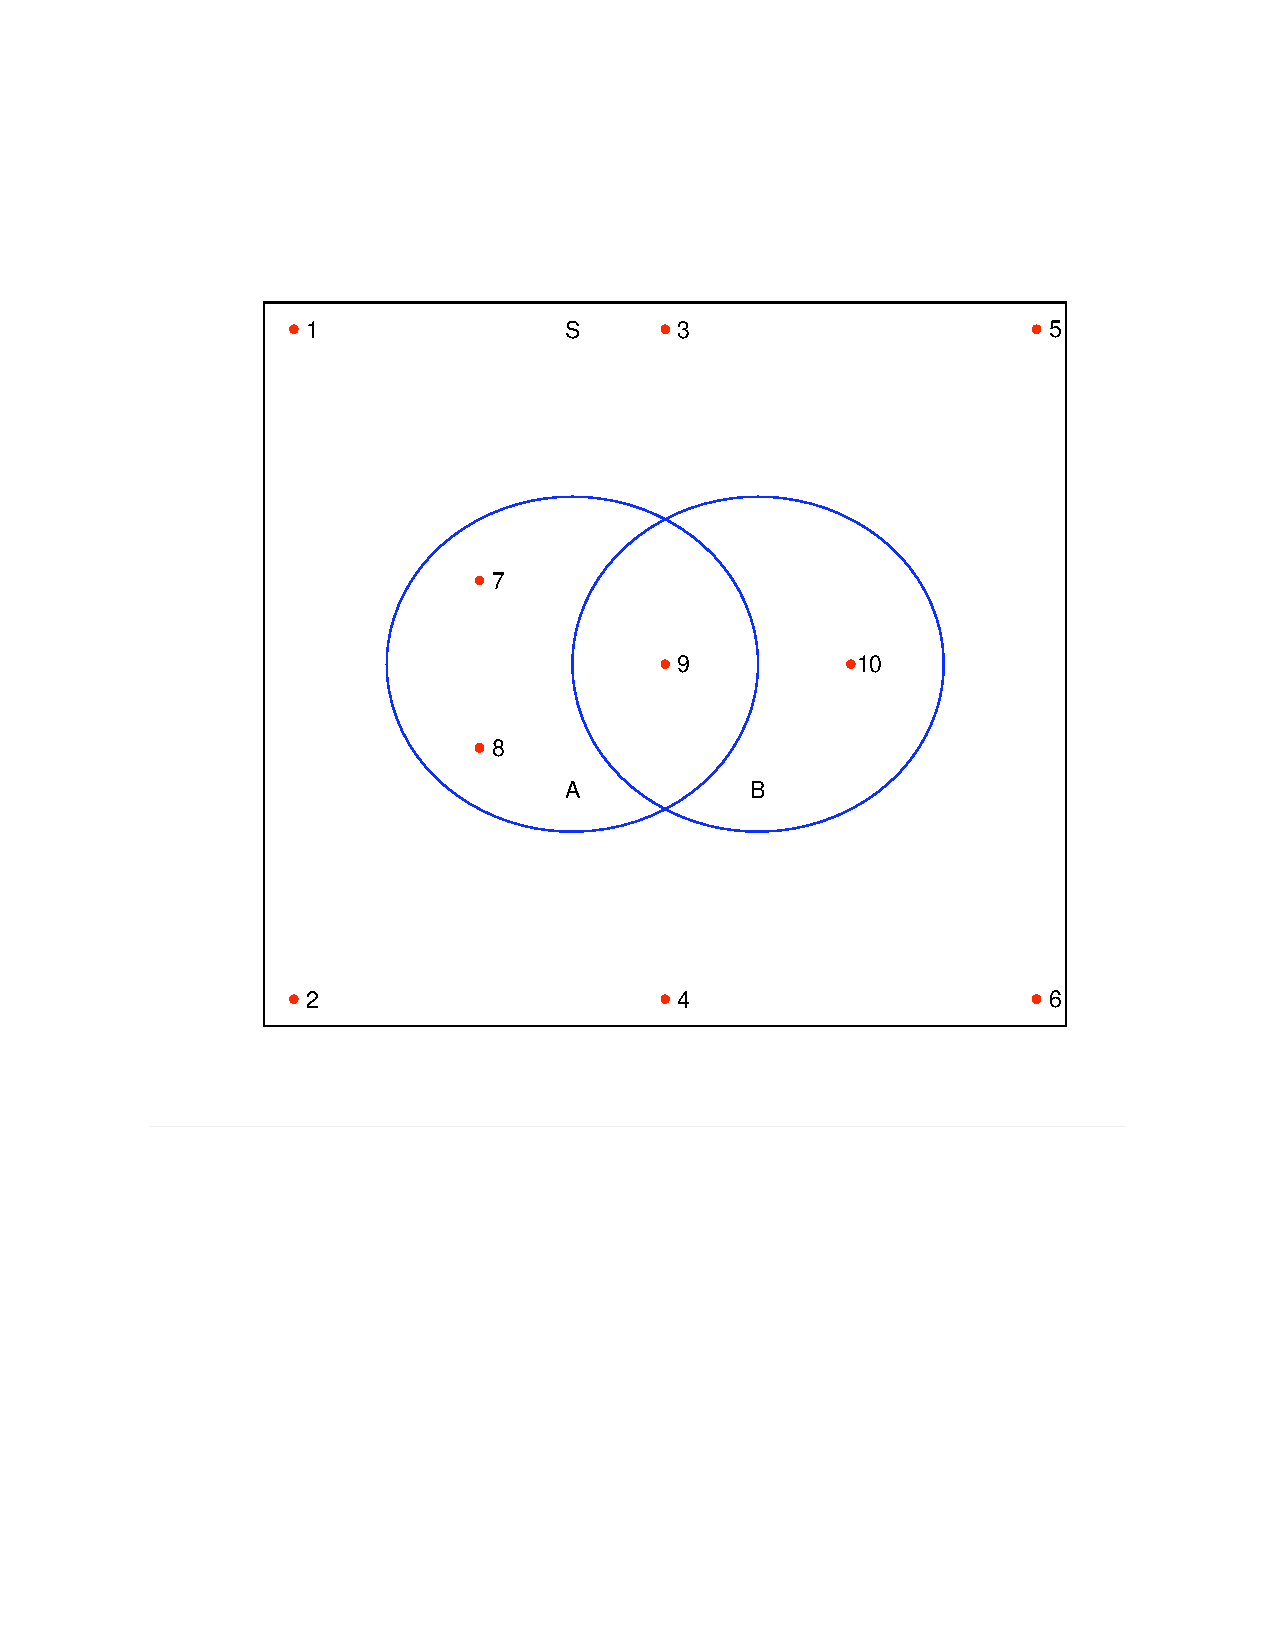
\includegraphics[height=12cm]{Section3/a2-fig-1}
%
%%\end{frame}
%\subsection{Two-way table}
%
%%\begin{frame} %[shrink=5]
%%frametitle{Two-way table}
%
%\noindent A very informative procedure for representing probabilities is
%a \textbf{two way table}.%\pause
%
%\begin{center}
%\begin{tabular}{|c|c|c|c|c|}\hline
%$B/A$&$A_1$&$\cdots$&$A_k$&total\\ \hline
%$B_1$&&$\cdots$&&\\ \hline
%$\cdots$&$\cdots$&$\cdots$&$\cdots$&$\cdots$\\ \hline
%$B_l$&&$\cdots$&&\\ \hline
%total&&$\cdots$&&\\ \hline
%\end{tabular}
%\end{center}
%
%%\end{frame}
%
%%\begin{frame} %[shrink=5]
%%\frametitle{Example of a two-way table}
%
%\noindent Suppose we want to measure income against age.  In one group we have
%under 50 group, and 50 and over group.  We can measure income as less than
%\$50,000, and \$50,000 and over.
%
%\begin{center}
%\begin{tabular}{|c|c|c|c|}\hline
%Income/Age&$A_1=\{< 50\}$&$A_2=\{\geq 50\}$&total\\ \hline
%$B_1=\{< \$50K\}$&40&10&50 \\ \hline
%$B_2=\{\geq \$50K\}$&5&45&50\\ \hline
%total&45&55&100\\ \hline
%\end{tabular}
%\end{center}
%
%%\end{frame}
%\subsection{Complementary Events}
%
%%\begin{frame} \frametitle{Complementary Events}%\pause
%
%For some event $A$ we denote it's \textbf{complementary event} by $A^c$, and what this means is all elements of
%$S$ that are not in, or complementary to $A$.% \pause
%
%\medskip
%
%We note that the probabilities of an event and it's complementary event is
%\[
%P(A)+P(A^c) = 1.
%\]
%
%
%%\end{frame}
%
%%\begin{frame}[<+->] \frametitle{Examples}
%
%%Will  be given in class.
%
%%\end{frame}
%\subsection{Mutually exclusive}
%
%%\begin{frame} \frametitle{Mutually exclusive}%\pause
%
%We have what is called the \textbf{additive rule} which asserts that given two events $A$ and $B$ if we form
%a third event $A\cup B$ then
%\[P\left(A\cup B\right) = P(A) + P(B) - P\left(A\cap B\right).\]%\pause
%
%\medskip
%
%Two events $A$ and $B$ are \textbf{mutually exclusive} if $A\cap B$ has no sample points.  In this case
%$P(A\cap B) =0$ so that the \textbf{probability of mutually exclusive events}
%\[P\left(A\cup B\right) = P(A) + P(B) .\]
%
%%\end{frame}
%
%%\begin{frame}[<+->] \frametitle{Examples}
%
%%\vspace{- 1.5 cm}
%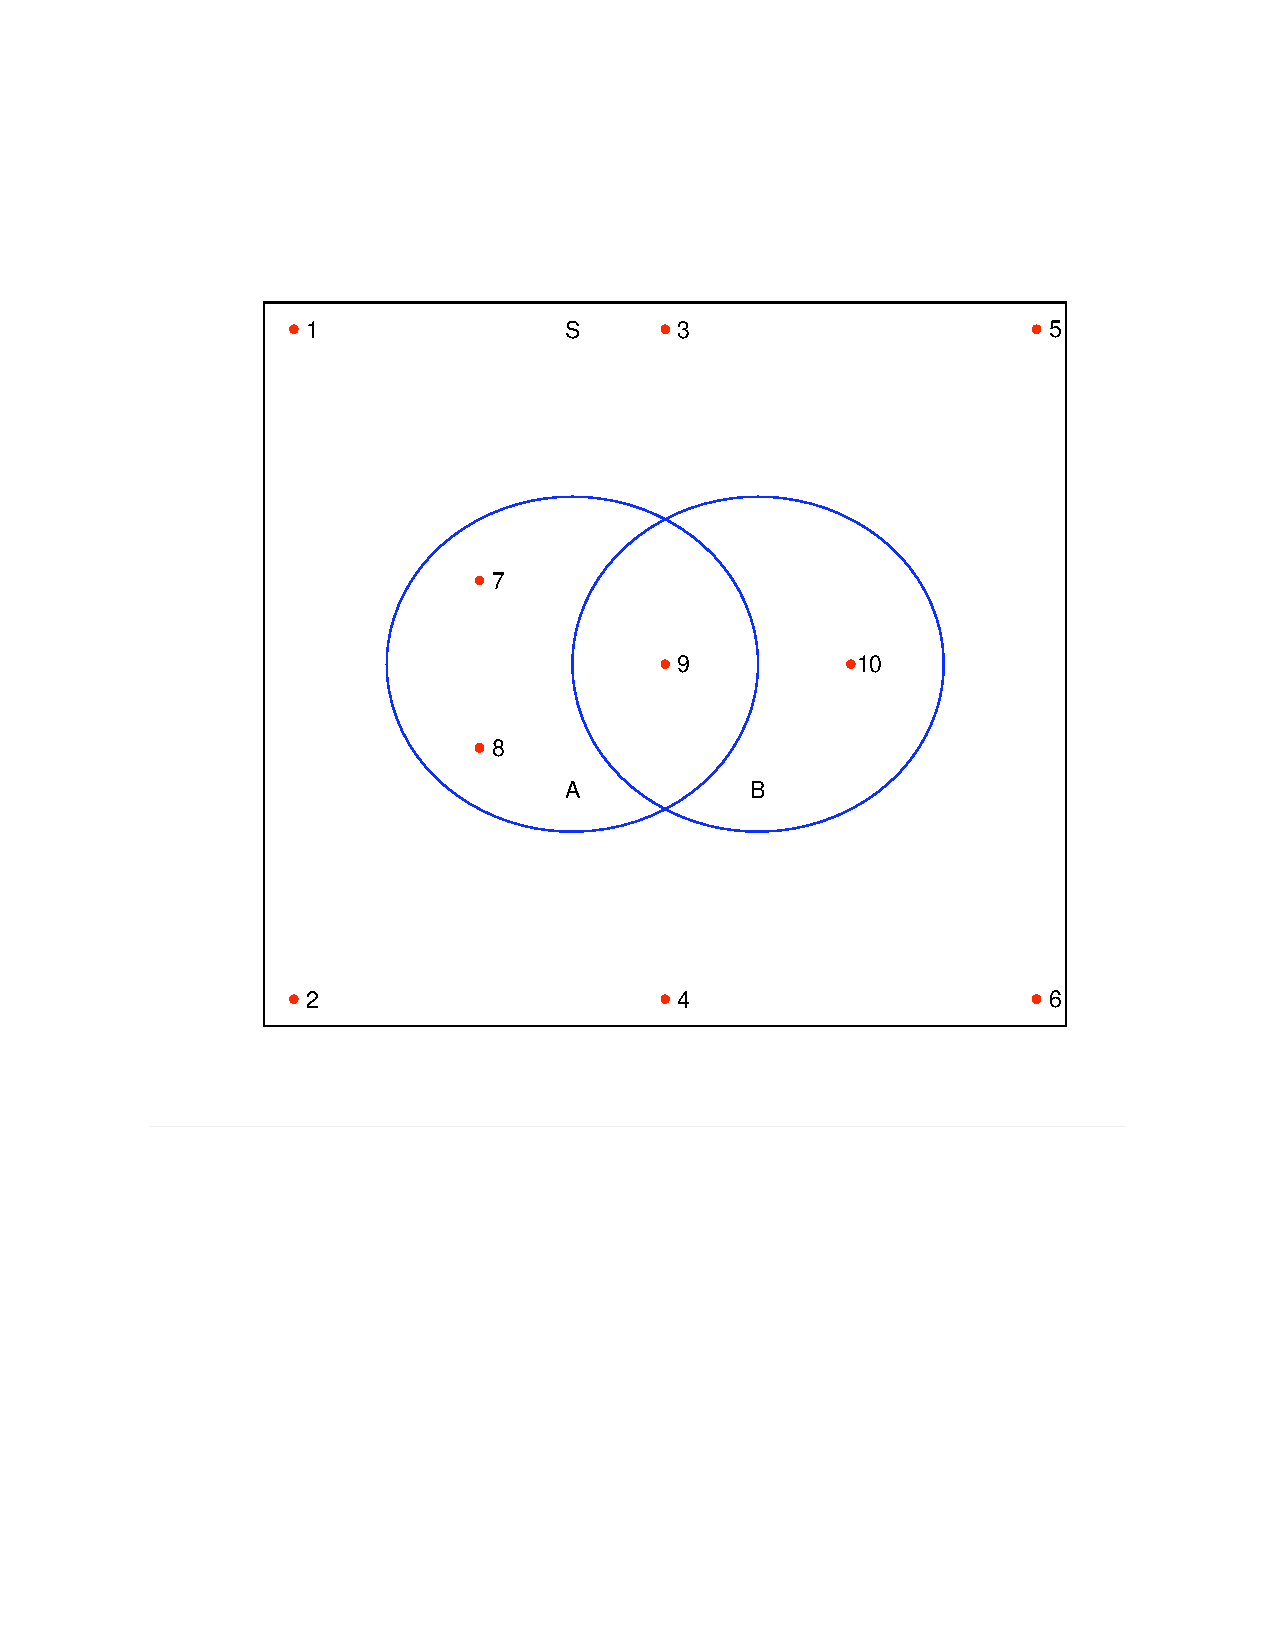
\includegraphics[height=12cm]{Section3/a2-fig-1}
%%\end{frame}
%
%%\begin{frame}[<+->] \frametitle{ }
%
%%\vspace{- 1 cm}
%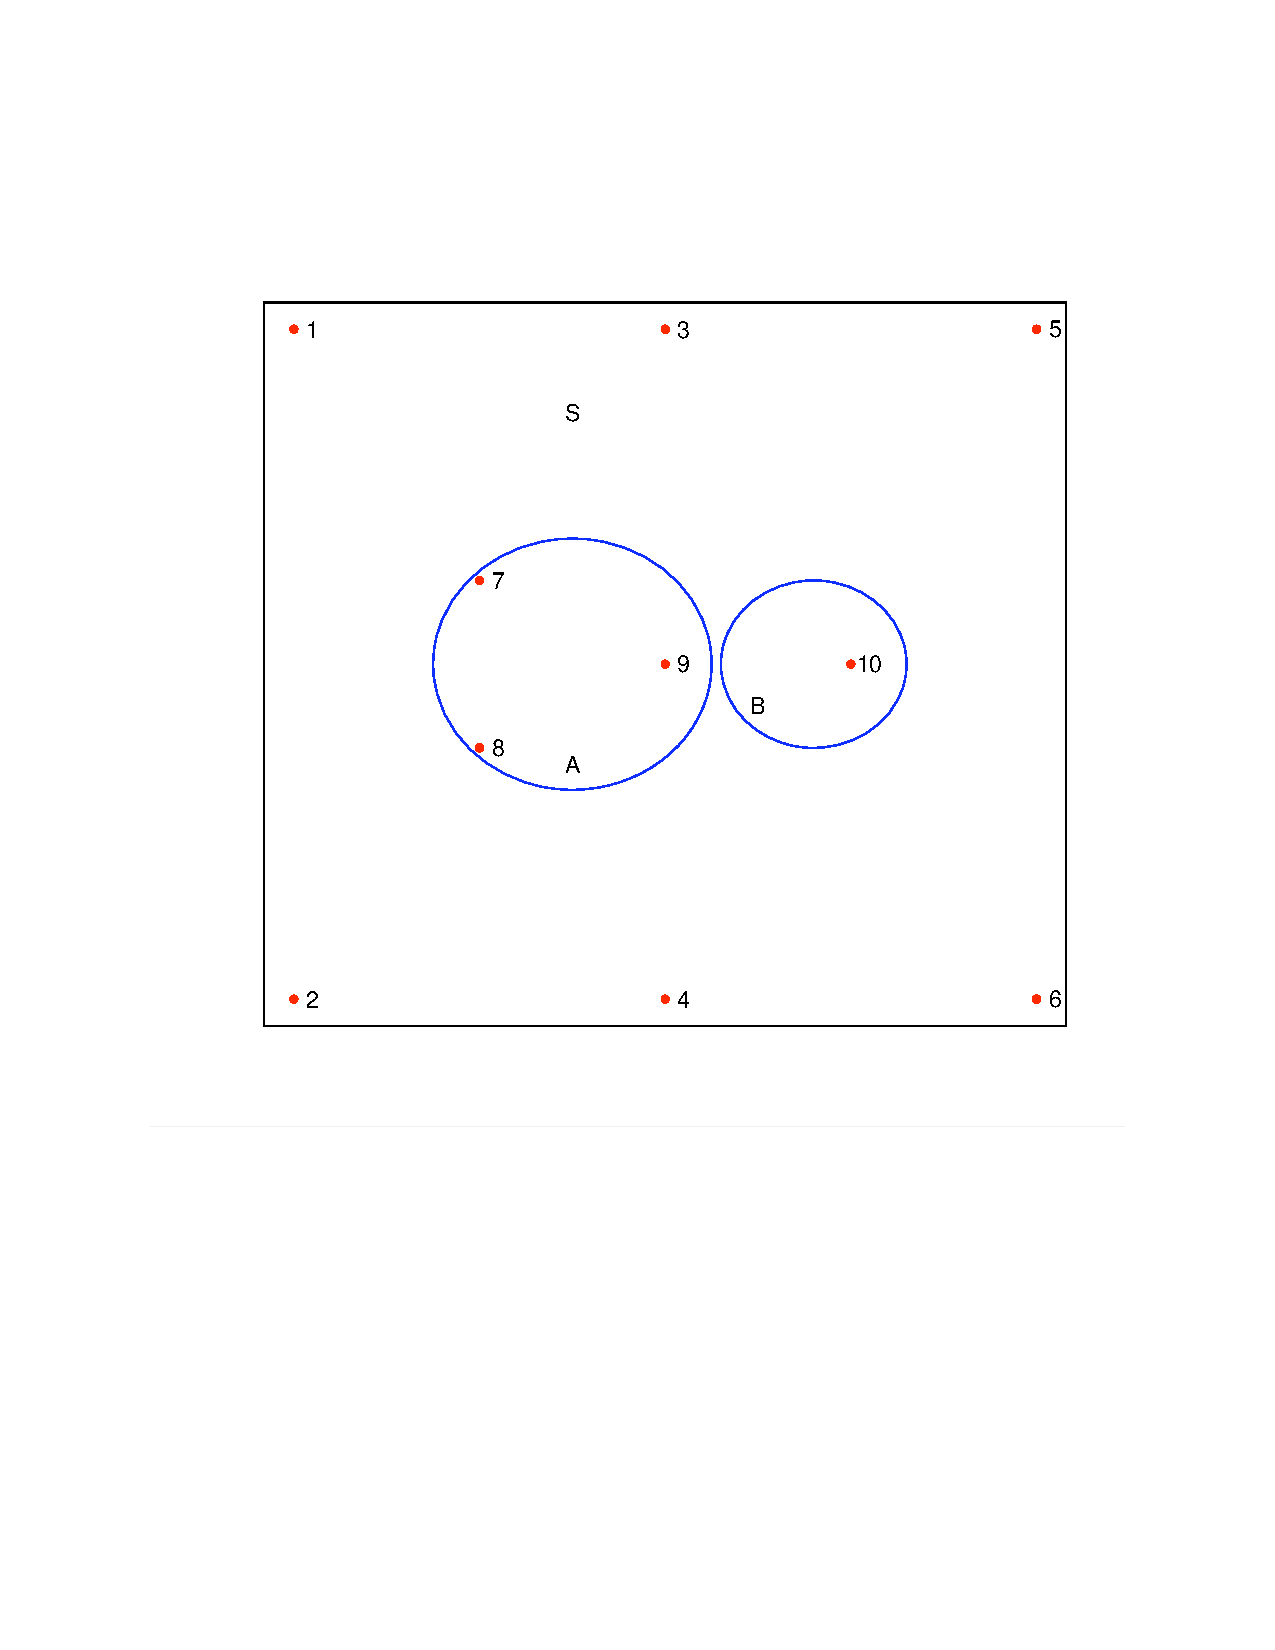
\includegraphics[height=12cm]{Section3/a2-fig-3}
%
%%\end{frame}
%
%%\begin{frame}[<+->] \frametitle{ }
%
%%\vspace{- 1 cm}
%\includegraphics[height=12cm]{Section3/a2-fig-2}
%
%%\end{frame}
%




\subsection{Exercises}
\begin{enumerate}
\item Suppose $P(A)=0.5$,$P(B)=0.8$,and $P(A\bigcap B)=0.4$.Find the following probabilities:
\begin{enumerate}
\item Find $P(A^{c})$ 
\item Find $P(A\bigcup B)$
\item Find $P(A\bigcap B^{c})$
\end{enumerate}

\item An experiment is conducted in which the outcomes of each of the two variables are observed.The two variables are Gender \{Male,Female\} and Age\{$\leq 30$,30-50,$\geq50$\}.The probabilities associated with each of the six possible outcome pairs are given as follows:
\begin{center}
\begin{tabular}{|c|c|c|c|}\hline
             &$\leq 30$&30-50&$\geq50$\\ \hline   
Male         &0.50     &0.10 &0.05\\ \hline
Female       &0.25     &0.07 &0.03\\ \hline
\end{tabular}
\end{center}
\begin{enumerate}
\item Find $P$(\{Male\})
\item Find $P$(\{Female or 30-50\})
\item Find $P$(\{$\leq$ 30\})
\item Find $P$(\{$\leq$ 30 and Female\})
\end{enumerate}


\item A pair of fair dice is tossed.Considering the following events:\\
%\begin{description}
$A$: \{The sum of the dots on the up faces of the two dice is 8\}.\\
$B$: \{at least one of the two dice showing is 3\}.

% \end{description}

\begin{enumerate}
\item Identify the sample points in the events $A,B,A\bigcap B,A\bigcup B$,and $A^{c}$.
\item Find the corresponding probabilities in part (a). 
\item Apply additive rule to $P$($A \bigcup B$).
\item Are the events $A$ and $B$ mutually exclusive?Why?
\end{enumerate}



\iffalse
\item Two balls are drawn at random and without replacement from a box containing two blue balls and two red balls.
\begin{enumerate}
\item List the sample points for this experiment.
\item Assign probabilities to the sample points.
\item Find the probability of the following events:
\begin{enumerate}
\item \{two red balls are drawn\}
\item \{One red and one blue are drawn\}
\item \{two balls with the same color are drawn\}
\end{enumerate}
\item The diagram below describes the sample space of a particular experiment and events A and B.
\begin{enumerate}
\item What is the name of the diagram?
\item Assume the sample points have the same probability.Find P(A),P(B) and P(C) .

\end{enumerate}
\end{enumerate}
\fi
%\item Show that if two $n \times n$ matrices $L$, $M$ are symmetric, then so are $L+M$ and $kL$.

\end{enumerate}
%\includegraphics[height=12cm]{a2-fig-2}
\iffalse
\label{se1} \markright{\ref{se1}
\titleref{se1}}
For the following exercises, let\\ $A=[1\ 2],\ B=\left[
\begin{array}{c}3\\2 \end{array}\right ],\ C=\left [\begin
{array}{rr} 1&-2\\2&-3\end {array} \right ],\ D=\left [\begin
{array}{rr} -2&-5\\1&3\end {array} \right ],\\ E=\left [\begin
{array}{rr} 1&5\\3&8
\\2&1\end {array}\right ],\
F=\left [\begin {array}{rrr} 2&-4&1\\6&-9&1\\4&1&6\\1&7&-5\end {array}\right],\
G=\left [\begin {array}{rrr} 1&2&6\\2&-3&7
\\4&-1&3\end {array}\right ],\\
H=\left [\begin {array}{rrr} 1&0&0\\0&1&0
\\-1&0&0\end {array}\right ],\
I=\left [\begin {array}{rrr} 1&0&0\\0&1&0
\\0&0&1\end {array}\right ],\
K=\left [\begin {array}{rrrr} 1&-2&4&7\\2&3&5&-4
\\1&4&2&1\\-2&1&9&4\end {array}
\right ].$
\bigskip

\begin{enumerate}
\item Which of the following operations are not defined? If they
are defined, what is the size of the resulting matrix
\begin{enumerate}
\item $AC$
\item $CA$
\item $KF^t$
\item $KF$
\item $EB+A^t$
\item $E(H+I)$
\end{enumerate}
\item Find: a) $C+D$\quad b) $D+C$ \quad  c) $G+H$ \quad
d) $D-3C$ \quad e) $2D$
\item Find:
\begin{enumerate} \item $AB$ and $BA$
\item $(C+2D)+BA$ and $C+(2D+BA)$
\item $DC$, $ED$, $(ED)C$ and $E(DC)$
\item $FH+FG$ and $F(G+H)$
\item $G^t$, $H^t$, $(GH)^t$, $G^tH^t$ and $H^tG^t$.
\end{enumerate}
\item Find: $KF$, $FG$ and $FH$.
\item Find tr($K$), tr($I$) and tr($E$).
\item Find $C^3$ and $H^2$.
\item Find $I-H$  and $(I-H)^2$.
\item If $f(x)=x^{2} +2x+2$, $g(x)=x^{2}-x-1$, find
\begin{enumerate} \item $f(C), {\rm (b)}~f(D), {\rm (c)}~g(C), {\rm (d)}~g(D)$.
\end{enumerate}
\item Show that if two $n \times n$ matrices $L$, $M$ are symmetric, then so are $L+M$ and $kL$.

\end{enumerate}



\iffalse
\section{Maple Exercises (optional)}

As in the previous session, first open the linear algebra package.

\begin{maplegroup}
\begin{mapleinput}
\mapleinline{active}{1d}{with(linalg):}{%
}
\end{mapleinput}

\end{maplegroup}
\bigskip

In this chapter, matrix operations and the matrix form of a linear
system ( $A{\bf x}={\bf b}$) were introduced.

We will begin this session by giving a second command to construct
a matrix (the first command was given during the previous Maple
session).

\bigskip

\begin{maplegroup}
\begin{mapleinput}
\mapleinline{active}{1d}{A := matrix(3,3, [1,2,3,2,3,4,3,4,5]);}{%
}
\end{mapleinput}

\mapleresult
\begin{maplelatex}
\[
A :=  \left[ {\begin{array}{rrr} 1 & 2 & 3 \\ 2 & 3 & 4 \\ 3 & 4 &
5
\end{array}}
 \right]
\]
\end{maplelatex}

\end{maplegroup}
\begin{maplegroup}
\begin{mapleinput}
\mapleinline{active}{1d}{B:=matrix(3,3,[2,5,7,13,3,5,6,7,8]);}{%
}
\end{mapleinput}

\mapleresult
\begin{maplelatex}
\[
B :=  \left[ {\begin{array}{rrr} 2 & 5 & 7 \\ 13 & 3 & 5 \\ 6 & 7
& 8
\end{array}}
 \right]
\]
\end{maplelatex}

\end{maplegroup}
\begin{maplegroup}
\begin{mapleinput}
\mapleinline{active}{1d}{C:=matrix(4,3,[1,3,5,7,9,0,8,6,4,2,1,7]);}{%
}
\end{mapleinput}

\mapleresult
\begin{maplelatex}
\[
C :=  \left[ {\begin{array}{rrr} 1 & 3 & 5 \\ 7 & 9 & 0 \\ 8 & 6 &
4 \\ 2 & 1 & 7
\end{array}}
 \right]
\]
\end{maplelatex}

\end{maplegroup}
\begin{maplegroup}
\begin{mapleinput}
\mapleinline{active}{1d}{E:=matrix(3,4,[3,4,7,6,9,2,8,2,6,8,3,12]);}{%
}
\end{mapleinput}

\mapleresult
\begin{maplelatex}
\[
E :=  \left[ {\begin{array}{rrrr} 3 & 4 & 7 & 6 \\ 9 & 2 & 8 & 2
\\ 6 & 8 & 3 & 12
\end{array}}
 \right]
\]
\end{maplelatex}

\end{maplegroup}
\bigskip

{\bf Note:} You can not let a matrix be $D$, a Maple error will
result.

Now that we have a few matrices at hand, we will perform some
matrix operations on them. First, scalar multiplication and matrix
addition. These operations are accomplished using the commands:
scalarmul(\emph{matrix name}, \emph{scalar value}) and
matadd(\emph{matrix name},\emph{matrix name}).

\bigskip

\begin{maplegroup}
\begin{mapleinput}
\mapleinline{active}{1d}{scalarmul(B,2);}{%
}
\end{mapleinput}

\mapleresult
\begin{maplelatex}
\[
 \left[
{\begin{array}{rrr} 4 & 10 & 14 \\ 26 & 6 & 10 \\ 12 & 14 & 16
\end{array}}
 \right]
\]
\end{maplelatex}

\end{maplegroup}
\begin{maplegroup}
\begin{mapleinput}
\mapleinline{active}{1d}{matadd(A , B);}{%
}
\end{mapleinput}

\mapleresult
\begin{maplelatex}
\[
 \left[
{\begin{array}{rrr} 3 & 7 & 10 \\ 15 & 6 & 9 \\ 9 & 11 & 13
\end{array}}
 \right]
\]
\end{maplelatex}

\end{maplegroup}
\bigskip

The `matadd' command can also be used to add scalar multiples of
one matrix to another matrix in the following way.
\bigskip

\begin{maplegroup}
\begin{mapleinput}
\mapleinline{active}{1d}{matadd(3*A,-B);}{%
}
\end{mapleinput}

\mapleresult
\begin{maplelatex}
\[
 \left[
{\begin{array}{rrr} 1 & 1 & 2 \\ -7 & 6 & 7 \\ 3 & 5 & 7
\end{array}}
 \right]
\]
\end{maplelatex}

\end{maplegroup}
\begin{maplegroup}
Matrix multiplication is performed using the `multiply' command.

\end{maplegroup}
\begin{maplegroup}
\begin{mapleinput}
\mapleinline{active}{1d}{multiply(A,B);}{%
}
\end{mapleinput}

\mapleresult
\begin{maplelatex}
\[
 \left[
{\begin{array}{rrr} 46 & 32 & 41 \\ 67 & 47 & 61 \\ 88 & 62 & 81
\end{array}}
 \right]
\]
\end{maplelatex}

\end{maplegroup}
\begin{maplegroup}
\begin{mapleinput}
\mapleinline{active}{1d}{multiply(A,B,E);}{%
}
\end{mapleinput}

\mapleresult
\begin{maplelatex}
\[
 \left[
{\begin{array}{rrrr} 672 & 576 & 701 & 832 \\ 990 & 850 & 1028 &
1228 \\ 1308 & 1124 & 1355 & 1624
\end{array}}
 \right]
\]
\end{maplelatex}

\end{maplegroup}
\bigskip

As shown in the previous section, Maple can be used to solve
systems of equations using the row reduction technique. A second
method uses the `linsolve' command. If we have the system $A{\bf
x}={\bf b}$, this command solves for {\bf x}. This command will be
demonstrated with the matrix $B$ from above, and a row matrix or
vector, $b$.

\bigskip

\begin{maplegroup}
\begin{mapleinput}
\mapleinline{active}{1d}{b:=vector([2,3,6]);}{%
}
\end{mapleinput}

\mapleresult
\begin{maplelatex}
\[
b := [2, \,3, \,6]
\]
\end{maplelatex}

\end{maplegroup}
\begin{maplegroup}
\begin{mapleinput}
\mapleinline{active}{1d}{linsolve(B,b);}{%
}
\end{mapleinput}

\mapleresult
\begin{maplelatex}
\[
 \left[  \! {\displaystyle \frac {29}{119}} , \,{\displaystyle
\frac {260}{119}} , \,{\displaystyle -\frac {160}{119}}  \!
 \right]
\]
\end{maplelatex}

\end{maplegroup}
\bigskip

Try solving the same system using the techniques and commands of
the previous Maple session.

The transpose of a matrix was also defined in this section. On
Maple, the transpose of a matrix is found with the `transpose'
command.
\bigskip

\begin{maplegroup}
\begin{mapleinput}
\mapleinline{active}{1d}{transpose(A);}{%
}
\end{mapleinput}

\mapleresult
\begin{maplelatex}
\[
 \left[
{\begin{array}{rrr} 1 & 2 & 3 \\ 2 & 3 & 4 \\ 3 & 4 & 5
\end{array}}
 \right]
\]
\end{maplelatex}

\end{maplegroup}
\begin{maplegroup}
\mapleresult
\begin{maplettyout}
\end{maplettyout}

\end{maplegroup}
\bigskip

Again you might want to try some other examples for yourself.  You
can also combine the commands to simplify long strings of
calculations. \fi

\section{Answers to activity questions and suggested exercises}
\label{answers2}

{\bf Activity questions}

\bigskip

\noindent {\bf \ref{ssec.arith}:} \quad 1.Yes.

\bigskip

\noindent{\bf \ref{ssec.propma}:} \quad Yes.

\bigskip


\noindent{\bf Suggested exercises}

\begin{enumerate}
\item \begin{enumerate}
\item $1 \times 2$
\item undefined
\item undefined
\item $4 \times 3$
\item undefined
\item undefined \end{enumerate}
\item a) $\left [\begin {array}{rr} -1&-7\\3&0\end {array}
\right ]$
b) $\left [\begin {array}{rr} -1&-7\\3&0\end {array}
\right ]$
c) $\left [\begin {array}{rrr} 2&2&6\\2&-2&7
\\3&-1&3\end {array}\right ]$
\\
d) $\left [\begin {array}{rr} -5&1\\-5&12\end {array} \right ]$ e)
$\left [\begin {array}{rr} -4&-10\\2&6\end {array} \right ]$
\item  \begin{enumerate} \item $7$, $\quad \left [\begin {array}{rr} 3&6\\2&4\end {array} \right ]$
\item $\left [\begin {array}{rr} 0&-6\\6&7\end {array}
\right ]$
\item  $\left [\begin {array}{rrr} -12&19\\7&-11\end {array}
\right ]$,  $\left [\begin {array}{rrr} 3&10\\2&9
\\-3&-7\end {array}\right ]$,  $\left [\begin {array}{rr} 23&-36\\20&-31
\\-17&27\end {array}\right ]$,  $\left [\begin {array}{rr} 23&-36\\20&-31
\\-17&27\end {array}\right ]$
\item $\left [\begin {array}{rrr} -1&11&-13\\-3&29&-24
\\28&0&49\\1&-7&40\end {array}
\right ]$, \quad $\left [\begin {array}{rrr} -1&11&-13\\-3&29&-24
\\28&0&49\\1&-7&40\end {array}
\right ]$
\item $G^t=\left [\begin {array}{rrr} 1&2&4\\2&-3&-1
\\6&7&3\end {array}\right ]$, \quad $H^t=\left [\begin {array}{rrr} 1&0&-1\\0&1&0
\\0&0&0\end {array}\right ]$, \\$(GH)^t=\left [\begin {array}{rrr} -5&-5&1\\2&-3&-1
\\0&0&0\end {array}\right ]$ \\

$G^tH^t=\left [\begin {array}{rrr} 1&2&-1\\2&-3&-2
\\6&7&-6\end {array}\right ]$, \quad $H^tG^t=\left [\begin {array}{rrr} -5&-5&1\\2&-3&-1
\\0&0&0\end {array}\right ]$
\end{enumerate}
\item $KF=\left [\begin {array}{rrr} 13&67&-12\\38&-58&55
\\35&-31&12\\42&36&33\end {array}
\right ]$, \quad  $FG=\left [\begin {array}{rrr}
-2&15&-13\\-8&38&-24
\\30&-1&49\\-5&-14&40\end {array}
\right ]$, \\ $FH=\left [\begin {array}{rrr} 1&-4&0\\5&-9&0
\\-2&1&0\\6&7&0\end {array}\right
]$
\item $10$, $3$, $E$ is not square
\item $C^3=\left [\begin {array}{rr} 5&-6\\6&-7\end {array}
\right ]$,\quad $H^2=\left [\begin {array}{rrr} 1&0&0\\0&1&0
\\-1&0&0\end {array}\right ]$
\item $\left [\begin {array}{rrr} 0&0&0\\0&0&0
\\1&0&1\end {array}\right ]$

\item a) $\left [\begin {array}{rr} 1&0\\0&1\end {array} \right ]$
b) $\left [\begin {array}{rr} -3&-15\\3&12\end {array} \right ]$
c) $\left [\begin {array}{rr} -5&6\\-6&7
\\\end {array}\right ]$
d) $\left [\begin {array}{rr} 0&0\\0&0\end {array} \right ]$

\item $(L+M)^{t}=L^{t}+M^{t}=L+M$, $(kL)^{t}=kL^{t}=kL$.
\end{enumerate}

%\end{document}
\fi 
%
%%\iffalse
%%\subsection{Exercises}
%%
%%%\begin{frame}\frametitle{Exercises}
%%
%%\noindent Exercises:
%%
%%\bigskip
%%
%%\noindent 11th edition, p. 127:  3.1-3.3, 3.6, 3.7
%%
%%\bigskip
%%
%%\noindent 10th edition, p. 143:  3.1-3.3, 3.6, 3.7
%%
%%
%%\end{frame}
%%\fi
%\section{Conditional Probability and Independence}
%
%\subsection{Conditional Probability}
%
%%\begin{frame}
%%\frametitle{Conditional Probability}%\pause
%
%For events $A$ and $B$ we have the notion of a
%\textbf{conditional probability} of $A$ given that the event $B$ has occurred.%\pause
%
%\medskip
%
%We can express this through the following
%\[
%P\left(A| B\right) = \frac{P\left(A\cap B\right)}{P(B)},
%\]
%where it is assumed that $P(B) \neq 0$.
%
%%\end{frame}
%
%%\begin{frame}[<+->] \frametitle{Examples}
%
%%\vspace{- 1 cm}
%\includegraphics[height=12cm]{Section3/a2-fig-2}
%
%%\end{frame}
%
%\subsection{Independence}
%%\begin{frame} \frametitle{Independence}%\pause
%
%We can re-express the conditional probability statement as a
%\textbf{multiplicative rule of probability}
%\[
% P\left(A\cap B\right) = P\left(A| B\right)P(B).
%\] %\pause
%
%\medskip
%
%The two events $A$ and $B$ are said to be \textbf{independent} if
%\[
% P\left(A| B\right) = P(B) \ \mbox{mistake should be}\ P(A),
%\]
%otherwise they are called \textbf{dependent}.%\pause
%
%\medskip
%
%The \textbf{probability of intersection of two independent events} has the very nice multiplicative property
%\[
% P\left(A \cap B\right) = P(A)P(B).
%\]
%
%%\end{frame}
%
%%\begin{frame}[<+->] \frametitle{Examples}
%
%%Will  be given in class.
%
%%\end{frame}
%
%%\begin{frame} %[shrink=5]
%%\frametitle{Example of a two-way table}
%
%\noindent Suppose we want to measure income against age.  In one group we have
%under 50 group, and 50 and over group.  We can measure income as less than
%\$50,000, and \$50,000 and over.
%
%\begin{center}
%\begin{tabular}{|c|c|c|c|}\hline
%Income/Age&$A_1=\{< 50\}$&$A_2=\{\geq 50\}$&total\\ \hline
%$B_1=\{< \$50K\}$&40&10&50 \\ \hline
%$B_2=\{\geq \$50K\}$&5&45&50\\ \hline
%total&45&55&100\\ \hline
%\end{tabular}
%\end{center}
%
%%\end{frame}
%

\subsection{Exercises}
\begin{enumerate}
\item For two events,$A$ and $B$,$P(A)=0.3$,$P(B)=0.2$,and$P(A\bigcap B)=0.1$.

\begin{enumerate}
\item Find $P(A\bigcup B)$.
\item Find $P(A|B)$.
\item Find $P(B|A)$.
\item Are $A$ and $B$ independent events?Justify your answer. 
\end{enumerate}
\item For two events,$A$ and $B$,$P(A)=0.4$,$P(B)=0.3$,and$P(A|B)=0.6$.

\begin{enumerate}
\item Find$P(A\bigcap B)$.
\item Find $P((B|A)$.
\end{enumerate}

\item For two independent events,$A$ and $B$,$P(A)=0.4$,$P(B)=0.3$.
\begin{enumerate}
\item Find $P(A\bigcup B)$.
\item Find $P(A|B)$.
\item Find $P(B|A)$.
\end{enumerate}



\item For two mutually exclusive events,$A$ and $B$,$P(A)=0.3$,$P(B)=0.7$.Find each of the following probabilities:
\begin{enumerate}
\item List the sample points for this experiment.
\item Find $P(A\bigcap B)$.
\item Find $P(B|A)$.
\item Find $P(A\bigcup B)$.
\end{enumerate}
%\item Show that if two $n \times n$ matrices $L$, $M$ are symmetric, then so are $L+M$ and $kL$.

\end{enumerate}



\iffalse
\begin{frame} \frametitle{Exercises}%\pause

\noindent Exercises:

\bigskip

\noindent 11th edition, p. 151:  3.47-3.51

\bigskip

\noindent 10th edition, p. 166:  3.41-3.45

\end{frame}
\fi 
%\section{Sampling}
%
%\subsection{Sampling}
%
%%\begin{frame} \frametitle{Sampling}%\pause
%
%In a population of size $N$ if a sample of size $n$ has equal probability of occuring, then the
%$n$ elements are called a
%\textbf{random sample}.
%
%%\end{frame}
%
%%\begin{frame}[<+->] \frametitle{Combinatorial rule}
%
%It is often the case than we wish to consider randomly drawing a sample of size $n$ from a
%population of size $N$.  %\pause
%
%\medskip
%
%A combinatorial rule for doing this is the following
%$$
%\left(
%\begin{array}{c}
%N\\
%n
%\end{array}
%\right) = \frac{N!}{(N-n)!n!}
%$$
%read as ``$N$ choose $n$", where $n!=n\cdot (n-1)\cdots 2\cdot 1$ called ``$n$ factorial".% \pause
%
%\medskip
%
%Another name used is \textbf{binomial coefficients}.
%
%%\end{frame}
%
%%\begin{frame}[<+->] \frametitle{Examples}
%
%Will  be given in class.
%
%%\end{frame}
%
%%\begin{frame} \frametitle{Exercises}%\pause
%

\subsection{Exercises}
\begin{enumerate}
\item Suppose a random sample of size 10 is selected from the population of size 10,000.Explain how you select your sample.

\item Suppose you wish to sample $n=4$ elements from a total of $N=600$ elements.

\begin{enumerate}
\item Compute the number of different samples.
\item If random sampling is to be employed,what is the probability that any particular sample will be selected?
\item Explain how you use a random number table to select the sample.
\item Explain how you use a computer to generate the sample.  
\end{enumerate}


%\item Show that if two $n \times n$ matrices $L$, $M$ are symmetric, then so are $L+M$ and $kL$.

\end{enumerate}



\iffalse
\begin{frame} \frametitle{Exercises}%\pause

\noindent Exercises:

\bigskip

\noindent 11th edition, p. 151:  3.47-3.51

\bigskip

\noindent 10th edition, p. 166:  3.41-3.45

\end{frame}
\fi 
%
%%\iffalse
%%\noindent Exercises:
%%
%%\bigskip
%%
%%\noindent 11th edition, p. 158:  3.76-3.79
%%
%%\bigskip
%%
%%\noindent 10th edition, p. 172:  3.68-3.71
%%
%%\end{frame}
%%\fi
%\section{Bayes rule}
%
%\subsection{Bayes rule}
%
%%\begin{frame} \frametitle{Bayes rule}%\pause
%
%A very useful formula is
%\textbf{Bayes rule} which is about turning conditional probabilities around.%\pause
%
%\medskip
%
%We know from before that
%\[
%P\left(A\cap B\right) = P\left(A| B\right)P(B).
%\] %\pause
%
%\medskip
%
%By definition we know
%
%\[
%P\left(B | A\right) = \frac{P\left(A\cap B\right)}{P(A)}
%=\frac{P\left(A| B\right)P(B)}{P(A)}.
%\]
%%\pause
%
%\medskip
%
%Therefore given information on $P(A|B)$, $P(A)$ and $P(B)$, we can recover $P(B|A)$.
%
%%\end{frame}
%
%%\begin{frame} \frametitle{Bayes rule continued}%\pause
%
%A generalization of Bayes rule to several events goes as follows. %\pause
%
%\medskip
%
%\noindent Suppose $B_1,\ldots , B_k$ are $k$ mutually exclusive events meaning
%$P(B_1)+\cdots +P(B_k)=1$.  Let $A$ be an observed event, then
%\begin{eqnarray}
%P\left( B_i |A\right) &=& \frac{P\left(B_i \cap A \right)}{P(A)}  \\
%&=& \frac{P\left(B_i  \right)P\left(A|B_i \right)}{P(B_1)P(A|B_1)+\cdots + P(B_k)P(A|B_k)}
%\end{eqnarray}
%for $i=1,\ldots,k$.
%
%%\end{frame}
%
%%\begin{frame}\frametitle{Example of a two-way table}
%
%\noindent Suppose we want to measure income against age.  In one group we have
%under 50 group, and 50 and over group.  We can measure income as less than
%\$50,000, and \$50,000 and over.
%
%\begin{center}
%\begin{tabular}{|c|c|c|c|}\hline
%Income/Age&$A_1=\{< 50\}$&$A_2=\{\geq 50\}$&total\\ \hline
%$B_1=\{< \$50K\}$&40&10&50 \\ \hline
%$B_2=\{\geq \$50K\}$&5&45&50\\ \hline
%total&45&55&100\\ \hline
%\end{tabular}
%\end{center}
%

\subsection{Exercises}
\begin{enumerate}
\item Suppose the events $A_1$ and $A_2$ ar mutually exclusive and complementary events.$P(A_1)=0.35$ and $P(A_2)=0.65$.Suppose another event $B$ such that $P(B|A_1)=0.3$ and $P(B|A_2)=0.5$

\begin{enumerate}
\item Find $P(B\bigcap A_1)$.
\item Find $P(B\bigcap A_2)$.
\item Find $P(B)$.
\item Find $P(A_1|B)$.
\item Find $P(A_2|B)$.
\end{enumerate}


\item Suppose the events $A_1$,$A_2$,and $A_3$ are mutually exclusive and complementary events.$P(A_1)=0.25$,$P(A_2)=0.15$,and $P(A_2)=0.60$.Suppose another event $B$ such that $P(B|A_1)=0.3$,$P(B|A_2)=0.25$,and $P(B|A_2)=0.55$.Use Bayes's Rule to find.
\begin{enumerate}
\item Find $P(A_1|B)$.
\item Find $P(A_2|B)$.
\item Find $P(A_3|B)$.
\end{enumerate}

\item Suppose the events $A_1$ and $A_2$ ar mutually exclusive and complementary events,such that $P(A_1)=0.35$ and $P(A_2)=0.65$.Suppose another event $P(B)=0.4$.If B is independent of $A_1$,$A_2$,then 

\begin{enumerate}
\item Find $P(A_1|B)$.
\item Find $P(A_2|B)$.
\end{enumerate}



\end{enumerate}



%\iffalse
%\begin{frame} \frametitle{Exercises}%\pause
%
%\noindent Exercises:
%
%\bigskip
%
%\noindent 11th edition, p. 151:  3.47-3.51
%
%\bigskip
%
%\noindent 10th edition, p. 166:  3.41-3.45
%
%\end{frame}
%\fi 
%%\end{frame}
%
%%\begin{frame} \frametitle{Exercises}%\pause
%
%%\noindent Exercises:
%
%%\bigskip
%
%%\noindent 11th edition, p. 161:  3.84-3.86
%
%%\bigskip
%
%%\noindent 10th edition, p. 176:  3.76-3.78
%
%%\end{frame}
%\section{Summary}\label{ssec.sumry2}
%\markright{\ref{ssec.sumry2} \titleref{ssec.sumry2}}
%{\bf Section Keywords: experiment;sample point;sample space;probability;event;\\simple event;compound event;probability of an event;
%trees;Venn diagrams;two way table;complementary event;additive rule;mutually exclusive;\\probability of mutually exclusive events;
%conditional probability;multiplicative rule of probability;dependent;probability of intersection of two independent events;
%random sample;binomial coefficients;Bayes rule.
%}
%
%%\iffalse
%%In the previous chapter, a system of linear equations was written in
%%matrix notation as $A{\bf{x}} = {\bf {b}}$.  If we were dealing
%%with numbers, rather than vectors and matrices, we would write
%%$ax=b$ and the solution (for $x$) would be $x = a^{-1}b$ provided
%%$a\neq0$.  It is natural to ask whether the equation $A{\bf{x}} =
%%{\bf{b}}$ has a solution ${\bf{x}} = A^{-1}{\bf{b}}$ for some
%%matrix $A^{-1}$.  The answer depends on the existence of a matrix
%%$A^{-1}$ with the property $A^{-1}A = AA^{-1} = I$.  Such a matrix
%%is called the inverse of $A$.  We will see how to calculate this
%%(when possible) and we will examine some of its properties.  The
%%determinant of a matrix will be introduced and some of the
%%properties of the determinant will be explored.  The determinant
%%gives an easy method for determining the existence of an inverse.
%%
%%\noindent {\bf Learning Objectives}
%%\noindent After completing this unit, you should be able to:
%%\begin{itemize}
%%\item understand what is meant by $A^{-1}$, and know how to find
%%whether one matrix is the inverse of another
%%\item define the words invertible, and singular
%%\item find the inverse of a matrix and know the properties of the inverse
%%\item relate invertibility to the solution of linear systems
%%\item find the determinant of a matrix
%%\item know the properties of the determinant
%%\item relate the value of the determinant to the invertibility of
%%a matrix.
%%\end{itemize}
%%
%%\section{Definition of an Inverse}
%%\label{ssec.definv}\markright{\ref{ssec.definv}
%%\titleref{ssec.definv}}
%%
%%In this section we define the inverse of a matrix. This
%%concept of invertibility will be very important throughout the
%%rest of the course.
%%
%%Let $A$ be a square matrix. If there exists a $B$ such that
%%$AB=BA=I$, then $A$ is said to be {\bf invertible}\index{invertible}. Furthurmore,
%%$B$ is called an {\bf inverse}\index{inverse} of $A$.
%%
%%Lets assume that the inverse of a matrix is not unique.  That is,
%%more than one $B$ exists such that $AB=BA=I$. For the matrix $A_{n
%%\times n}$, let two such inverses be $B_{n \times n}$ and $C_{n
%%\times n}$. We must have $(BA)=(AB)=I$ and $(CA)=(AC)=I$, since
%%$B$ and $C$ are both inverses of $A$. Now,
%%\begin{eqnarray}
%%C=IC&=&(BA)C\\&=&B(AC)=BI=B.
%%\end{eqnarray}
%%Therefore the two inverses must be equal, and the inverse unique.
%%
%%We have just shown that an inverse is unique. Hence, we speak of
%%`the inverse' and can denote the inverse by $A^{-1}$ without
%%ambiguity. This notation is intuitive; $A^{-1}$ plays an analogous
%%role to the real number $a^{-1} = \frac{1}{a}$, (when $a\neq0$)
%%since $aa^{-1}=1$ and $AA^{-1}=I$.
%%
%%An important feature of invertible mattrices is that they can be
%%cancelled from equations:
%%
%%If $AB = AC$ and $A$ is invertible, then multiplying on the left
%%by $A^{-1}$ gives
%%
%%\begin{eqnarray}
%%A^{-1}(AB) & = & A^{-1}(AC)\\
%%\mathrm{i.e.}\ (A^{-1}A)B & = & (A^{-1}A)C\\
%%\mathrm{i.e.}\ IB = IC&\mathrm{or}&B = C
%%\end{eqnarray}
%%
%%We have seen that B is the inverse of A $(B=A^{-1})$ if
%%$AB=BA=I$.  This same condition would show that A is the inverse of B
%%$(A=B^{-1})$.  Hence, $B=A^{-1}\Leftrightarrow A=B^{-1}$ and we say A and B
%%are inverses (of one another).
%%\begin{example}
%%\label{exam3.multinv} Are $A$ and $B$ inverses?
%% $$ A =\begin{bmatrix} -2 & 3 \\ -3 & 4
%%\end{bmatrix} \quad B = \begin{bmatrix} 4 & -3 \\ 3 & -2 \end{bmatrix}$$
%%\begin{align}
%%AB&= \begin{bmatrix}-2&3\\-3&4 \end{bmatrix}\,\begin{bmatrix}4&-3\\3&-2 \end{bmatrix}
%%=\begin{bmatrix}1&0\\0&1 \end{bmatrix}
%%\intertext{and}
%%BA&= \begin{bmatrix}4&-3\\3&-2 \end{bmatrix}\,\begin{bmatrix}-2&3\\-3&4\end{bmatrix}
%%=\begin{bmatrix}1&0\\ 0&1 \end{bmatrix}.
%%\end{align}
%%Therefore $A$ and $B$ are inverses.
%%\end{example}
%%In the definition above, it was stated that $B$ will be the
%%inverse if it exists.  Not all matrices will have inverses. A
%%matrix which does not have an inverse is called a {\bf singular}\index{singular}
%%matrix.  The following example gives a singular matrix.
%%
%%\begin{example}\label{exam3.noinv}
%%Consider the matrix
%%$$\begin{bmatrix}2&7&0\\6&4&0\\3&1&0 \end{bmatrix}.$$
%%Assume that $B$ is its inverse. Thus,
%%$$\begin{bmatrix}1&0&0\\0&1&0\\0&0&1 \end{bmatrix}=
%%  \begin{bmatrix}b_{11}&b_{12}&b_{13}\\
%%                 b_{21}&b_{22}&b_{23}\\
%%                 b_{31}&b_{32}&b_{33}
%%  \end{bmatrix}\,
%%  \begin{bmatrix}2&7&0\\
%%                 6&4&0\\
%%                 3&1&0
%%  \end{bmatrix}
%%$$
%%Equating the $(3, 3)$ places gives $0b_{31}+0b_{32}+0b_{33}=1$, i.e $0=1$. This is a contradiction.
%%Therefore, the matrix has no inverse.
%%\end{example}
%%
%%\noindent {\bf Activity \ref{ssec.definv}}
%%
%%\begin{enumerate}
%%\item Which sets of matrices are inverses?
%%\begin{enumerate}
%%\item $\left[ \begin{array}{rrr} 1&1&0\\-1&-1&3\\0&2&-1 \end{array} \right
%%], \quad \left [ \begin{array}{rrr}\vspace{1mm}
%%                    \frac{5}{6}&-\frac{1}{6}&-\frac{1}{2}\\\vspace{1mm}
%%                    \frac{1}{6}&\frac{1}{6}&\frac{1}{2}\\
%%                    \frac{1}{3}&\frac{1}{3}&0  \end{array} \right ]$
%%\item $\left [ \begin{array}{rr} 2&-1\\ -5&-3 \end{array} \right
%%], \quad \left [ \begin{array}{rr} 3&1 \\5&-2 \end{array} \right
%%]$
%%\end{enumerate}
%%\item What is the inverse of $I$?
%%\end{enumerate}
%%\noindent The answers can be found in section \ref{answers3}.
%%
%%\section{Finding the Inverse of a Matrix}
%%\label{ssec.findinv}\markright{\ref{ssec.findinv}
%%\titleref{ssec.findinv}}
%%
%%Although we have defined the inverse of a matrix, we have not yet
%%shown how to find it. For $2 \times 2$ matrices only, the following formula can
%%be used:
%%
%%Let $A$ be an invertible matrix
%%$$ A= \begin{bmatrix} a&b\\
%%                      c&d \end{bmatrix}.$$
%%Then its inverse is:
%%\begin{equation} \label{inv1}
%%A^{-1}= \frac{1}{ad-bc}\left [
%%\begin{array}{rr}
%%            d&-b\\
%%            -c&a \end{array} \right ].
%%\end{equation}
%%Verify that this is indeed the inverse by finding the
%%product $AA^{-1}$.
%%
%%\begin{example}
%%\label{exam3.findprod} Use {\rm (\ref{inv1})} to find $A^{-1}, B^{-1}\ and\ (AB)^{-1}$.
%%
%%$$\mbox{let } A= \begin{bmatrix}1&2\\ 3&4 \end{bmatrix}, \quad B= \begin{bmatrix}5&6\\ 7&8
%%\end{bmatrix},$$
%%
%%$$ \mbox{ then } AB= \begin{bmatrix} 19&22\\ 43&50
%%\end{bmatrix}.$$
%%
%%By \ref{inv1} we have....
%%$$A^{-1}=\frac{1}{1\cdot4-2\cdot3}\left[\begin{array}{rr}4&-2\\
%%-3&1\end{array}\right]=
%%-\frac{1}{2}\left[\begin{array}{rr}4&-2\\ -3&1 \end{array}\right]=\left[
%%\begin{array}{rr}-2&1\\ \frac{3}{2}&-\frac{1}{2} \end{array}\right ]$$
%%
%%$$ B^{-1} = \frac{1}{5\cdot8-6\cdot7} \left [ \begin{array}{rr} 8&-6\\ -7& 5\end{array}
%%\right ]=-\frac{1}{2} \left [ \begin{array}{rr} 8&-6\\ -7& 5\end{array}\right ]=
%%\left [ \begin{array}{rr} -4&3\\ \frac{7}{2}&-\frac{5}{2}\end{array}\right ]$$
%%
%%$$ (AB)^{-1} = \frac{1}{19\cdot50-22\cdot43}\left [ \begin{array}{rr} 50&-22\\ -43&
%%19\end{array} \right ]=\frac{1}{4}\left [ \begin{array}{rr} 50&-22\\ -43&
%%19\end{array} \right ]= \left [ \begin{array}{rr}\vspace{1mm} \frac{25}{2}&-\frac{11}{2}\\
%%\vspace{1mm}-\frac{43}{4}&\frac{19}{4}\end{array} \right ]$$
%%\end{example}
%%We will illustrate how to find the inverse of a $n \times n$ matrix $(n \geq 3)$ by means of an example when
%%$n=3$.
%%
%%\begin{example}
%%\label{exam4.findinv}
%%Find the inverse of
%%$$
%%\left[ \begin{array}{rrr} 1&2&1\\2&5&3\\-1&-1&1 \end{array} \right].
%%$$
%%We have to solve
%%$$
%%\left[ \begin{array}{rrr} 1&2&1\\2&5&3\\-1&-1&1 \end{array} \right]\,
%%\begin{bmatrix}a_1&b_1&c_1\\a_2&b_2&c_2\\a_3&b_3&c_3\end{bmatrix} =
%%\begin{bmatrix}1&0&0\\0&1&0\\0&0&1\end{bmatrix}.
%%$$
%%Writing the equations involving the $a$'s gives
%%\begin{equation}
%%\begin{aligned}
%%1a_1 + 2a_2 + 1a_3 &=1 \\
%%2a_1 + 5a_2 + 3a_3 &=0 \\
%%-1a_1 -1a_2 + 1a_3 &=0
%%\end{aligned},\ \mathrm{or}\
%%\left[ \begin{array}{rrrrr}
%%1&2&1&\vline&1\\
%%2&5&3&\vline&0\\
%%-1&-1&1&\vline&0
%%\end{array} \right].
%%\end{equation}
%%If we row--reduce, we obtain
%%$$
%%\begin{bmatrix}1&0&0&\vline&a_1\\0&1&0&\vline&a_2\\0&0&1&\vline&a_3\end{bmatrix}.
%%$$
%%The values $a_1,\,a_2,\,a_3$ appear in the last column because $x_1=a_1,\, x_2= a_2,\,x_3=a_3$ is the
%%solution to the system.  Similarly, for the $b$'s,
%%\begin{equation}
%%\begin{aligned}
%%1b_1 + 2b_2 + 1b_3 &=0 \\
%%2b_1 + 5b_2 + 3b_3 &=1 \\
%%-1b_1 -1b_2 + 1b_3 &=0
%%\end{aligned},\ \mathrm{or}\
%%\left[ \begin{array}{rrrrr}
%%1&2&1&\vline&0\\
%%2&5&3&\vline&1\\
%%-1&-1&1&\vline&0
%%\end{array} \right].
%%\end{equation}
%%If we row--reduce, we obtain
%%$$
%%\begin{bmatrix}1&0&0&\vline&b_1\\0&1&0&\vline&b_2\\0&0&1&\vline&b_3\end{bmatrix}.
%%$$
%%Exactly the same idea applies for the $c$'s.  The system of equations is
%%$$
%%\left[ \begin{array}{rrrrr}
%%1&2&1&\vline&0\\
%%2&5&3&\vline&0\\
%%-1&-1&1&\vline&1
%%\end{array} \right].
%%$$
%%and this reduces to
%%$$
%%\begin{bmatrix}1&0&0&\vline&c_1\\0&1&0&\vline&c_2\\0&0&1&\vline&c_3\end{bmatrix}.
%%$$
%%Since the reduction process is identical in each case, we may as well reduce all three at once:
%%\begin{align}
%%&\left[ \begin{array}{rrrrrrr}
%%1&2&1&\vline&1&0&0\\
%%2&5&3&\vline&0&1&0\\
%%-1&-1&1&\vline&0&0&1
%%\end{array} \right]
%%\quad\ \  \overset{\begin{smallmatrix}R_2-2R_1\\R_3+R_1\end{smallmatrix}}{\leadsto} \quad
%%&&\hspace{-10mm}\left[ \begin{array}{rrrrrrr}
%%1&2&1&\vline&1&0&0\\
%%0&1&1&\vline&-2&1&0\\
%%0&1&2&\vline&1&0&0
%%\end{array} \right] \\
%%\overset{\begin{smallmatrix}R_1-2R_2\\R_3-R_2\end{smallmatrix}}{\leadsto}
%%&\left[ \begin{array}{rrrrrrr}
%%1&0&-1&\vline&5&-2&0\\
%%0&1&1&\vline&-2&1&0\\
%%0&0&1&\vline&3&-1&1
%%\end{array} \right]
%%\quad \overset{\begin{smallmatrix}R_1+R_3\\R_2-R_3\end{smallmatrix}}{\leadsto} \quad
%%&&\hspace{-10mm}\left[ \begin{array}{rrrrrrr}
%%1&0&0&\vline&8&-3&1\\
%%0&1&0&\vline&-5&2&-1\\
%%0&0&1&\vline&3&-1&1
%%\end{array} \right]
%%\end{align}
%%Hence the inverse is
%%$$
%%\left[ \begin{array}{rrr}
%%8&-3&1\\
%%-5&2&-1\\
%%3&-1&1
%%\end{array} \right]
%%$$
%%\end{example}
%%This is the process of finding the inverse of $n \times n$ matrices with $n \geq 3$.  Symbolically, we have
%%$$
%%[A|I] \leadsto [I|A^{-1}] \quad \mathrm{by\ elementary\ row\ operations}.
%%$$
%%The algorithm for finding the inverse will now be demonstrated by another example.
%%\begin{example}\label{exam3.findinv}
%%Let
%%$$
%%A = \left [\begin{array}{rrr}
%%      1 & 0 & 2 \\
%%      2 & -1 & 3 \\
%%      4 & 1 & 8 \end{array} \right ].
%%$$ Find $A^{-1}$.
%%\\
%%\noindent {\bf Step 1.}  Set up the matrix $[ \ A \ |\ I \ ]$.
%%$$
%%\left[ \begin{array}{rrrcrrr} 1 & 0 & 2 & \vline & 1 & 0 & 0
%%\\ 2 & -1 & 3 & \vline & 0 & 1 & 0 \\ 4 & 1 & 8 & \vline & 0 & 0 & 1
%%\end{array} \right ]
%%$$
%%\noindent {\bf Step 2.}   Use elementary row operations to reduce
%%$[ \ A \ | \ I \ ]$ to $[ \ I \ | \ A^{-1} \ ]$.
%%$$
%%\begin{array}{rl}
%%\overset{\begin{smallmatrix}R_2-2R_1\\R_3-4R_1\end{smallmatrix}}{\leadsto}
%%&\left[ \begin{array}{rrrcrrr} 1 & 0 & 2 & \vline &1 & 0 & 0 \\ 0 & -1 &
%%-1 & \vline & -2 & 1 & 0 \\ 0 & 1 & 0 & \vline & -4 & 0 & 1
%%\end{array} \right]\\ &\\
%%\overset{-R_2}{\leadsto}  & \left[ \begin{array}{rrrcrrr} 1 &
%%0 & 2 & \vline & 1 & 0 & 0 \\ 0 & 1 & 1 & \vline & 2 & -1 & 0 \\ 0
%%& 1 & 0 & \vline & -4 & 0 & 1 \end{array} \right]\\ &\\
%%\overset{R_3-R_2}{\leadsto} & \left[ \begin{array}{rrrcrrr} 1 & 0
%%& 2 & \vline & 1 & 0 & 0 \\ 0 & 1 & 1 & \vline & 2 & -1 & 0 \\ 0 &
%%0 & -1 & \vline & -6 & 1 & 1
%%\end{array} \right]\\ &\\
%%\overset{-R_3}{\leadsto} &\left[ \begin{array}{rrrcrrr} 1 & 0
%%& 2 & \vline & 1 & 0 & 0 \\ 0 & 1 & 1 & \vline & 2 & -1 & 0 \\ 0 &
%%0 & 1 & \vline & 6 & -1 & -1
%%\end{array} \right]\\
%%&\\ \overset{\begin{smallmatrix}R_1-2R_3\\R_2-R_3\end{smallmatrix}}{\leadsto} & \left[
%%\begin{array}{rrrcrrr} 1 & 0 & 0 & \vline & -11 & 2 & 2 \\ 0 & 1 & 0 & \vline & -4 &
%%0 & 1 \\ 0 & 0 & 1 & \vline & 6 & -1 & -1
%%\end{array} \right].
%%\end{array}
%%$$
%%
%%\noindent {\bf Step 3.}  The matrix is now in the form $[ \ I \ |
%%\  A^{-1} \ ]$.  Therefore: $$ A^{-1}= \left [
%%\begin{array}{rrr}
%%           -11 & 2 & 2 \\
%%            -4 & 0 & 1 \\
%%             6 & -1 & -1 \end{array} \right ].
%%$$
%%Verify that this is true by finding $AA^{-1}.$
%%\end{example}
%%The latter procedure shows that the inverse $A^{-1}$ can be found precisely when $A$ can
%%be reduced to the identity matrix $I$.  If $A$ is an $n \times n$ matrix, then the following
%%statements are equivalent, \emph{i.e.}, if one of them is true they are all true, if one of them
%%is false they are all false.
%%\begin{enumerate}
%%\item $A$ is invertible.
%%\item $A$ is row equivalent to $I_n$
%%\item $A{\bf{x}} = 0 $ (the homogeneous system) has only the trivial solution.
%%\end{enumerate}
%%
%%These results imply that a square matrix which is not
%%invertible cannot be reduced to $I$ using elementary row
%%operations.  This has a practical use, since if at some point
%%during the computation of an inverse, a row of zeroes occurs on
%%the left side, then the matrix is not invertible and the
%%computation can be stopped.
%%
%%\begin{example} For the matrix given below, find its inverse, if it
%%exists.
%%
%%$$A=\left [ \begin{array}{rrr}
%%                1&2&0\\
%%                1&1&-2\\
%%                0&2&4 \end{array} \right ]$$
%%Set up the matrix $[\ A \ \vline \ I \ ]$ and reduce:
%%
%%$$
%%\begin{array}{rl}
%%& \left [ \begin{array}{rrrcrrr}
%%            1&2&0&\vline & 1&0&0\\
%%            1&1&-2& \vline & 0&1&0\\
%%            0&2&4& \vline & 0&0&1 \end{array} \right ]\\ &\\
%%\overset{R_2-R_1}{\leadsto}&\left [ \begin{array}{rrrcrrr}
%%            1&2&0&\vline & 1&0&0\\
%%            0&-1&-2& \vline & -1&1&0\\
%%            0&2&4& \vline & 0&0&1 \end{array} \right ]\\ &\\
%%\overset{R_3+2R_2}{\leadsto}&\left [ \begin{array}{rrrcrrr}
%%            1&2&0&\vline & 1&0&0\\
%%            0&-1&-2& \vline & -1&1&0\\
%%            0&0&0& \vline & -2&2&1 \end{array} \right ] \end{array}$$
%%A row of zeroes has occurred on the left hand side of the matrix,
%%therefore, this matrix is not invertible.
%%\end{example}
%%
%%\noindent {\bf Activity \ref{ssec.findinv}}
%%Find the inverses of the following matrices, or determine that the matrix is not invertible.
%%\begin{itemize}
%%\item[(a)] $\left[ \begin{array}{rrr}
%%                        1&0&1\\
%%                        -1&1&2\\
%%                        2&2&9 \end{array} \right]$
%%\item[(b)] $\left [ \begin{array}{rrr} 1&0&1\\ 1&1&0 \\ -1&1&-2 \end{array} \right ]$
%%\item[(c)] $\left [ \begin{array}{rrrr}
%%                        1&0&0&0\\
%%                        0&0&0&1 \\
%%                        0&0&1&0\\
%%                        0&1&0&0\end{array} \right ]$
%%\end{itemize}
%%\noindent The answers can be found in section \ref{answers3}.
%%
%%\section{Properties of the Inverse}
%%\label{ssec.propinv}\markright{\ref{ssec.propinv}
%%\titleref{ssec.propinv}}
%%
%%We now state some important properties about the inverse.
%%
%%If $A$, and $B$ are invertible matrices of the same size then:
%%\begin{enumerate}
%%
%%\item $AB$ is invertible.  In fact, the product of any number of
%%invertible matrices will be invertible.
%%\item $(AB)^{-1}=B^{-1}A^{-1}$.  This property can be extended to
%%the inverse of any product of invertible matrices.
%%\item If $B$ is square and $BA = I$, then $B = A^{-1}$.
%%\item If $B$ is square and $AB = I$, then $B = A^{-1}$.
%%\item $(A^{-1})^{-1}=A$.
%%\item $(A^n)^{-1}=(A^{-1})^n=A^{-n}$.
%%\item $(kA)^{-1}= \frac{1}{k}A^{-1},\ k \neq 0$.
%%\item $(A^t)^{-1}=(A^{-1})^t$.
%%\end{enumerate}
%%
%%It is easy to verify that some of these properties are in fact true. For
%%example, we have stated that $(AB)^{-1}=B^{-1}A^{-1}$. We know
%%that the inverse of $(AB)^{-1}$ is $AB$ and that the inverse is
%%unique. Now
%%$$ (AB)(B^{-1}A^{-1})=I \ {\rm and} \ (B^{-1}A^{-1})(AB)=I$$
%%so $B^{-1}A^{-1}$  must be the inverse to $AB$, which we have denoted
%%by $(AB)^{-1}$!
%%
%%Note that by properties 3 and 4, if you want to check that two matrices $A$ and $B$
%%are inverses, it is only necessary to check either $AB = I$ or $BA = I$ (and not both).
%%The fact is that
%%$$
%%AB = I \Leftrightarrow BA = I
%%$$
%%and then $A$ and $B$ are inverses.
%%
%%The following example uses property 6 to find the required matrix.
%%\begin{example} Given,
%%\label{exam3.invprop}
%% $$A= \left [
%%\begin{array}{rr} 2 & -1 \\ -3 & 2
%%\end{array}
%% \right], \quad A^{-1}=\left [
%%\begin{array}{rr} 2 & 1 \\ 3 & 2
%%\end{array}
%% \right ].$$
%% Find $A^{-3}$. $$ A^{-3}=(A^{-1})^3=\left [ \begin{array}{rr}
%%2&1
%%\\ 3&2 \end{array} \right ]\left [ \begin{array}{rr} 2&1 \\ 3&2 \end{array}
%%\right ]\left [ \begin{array}{rr} 2&1 \\ 3&2 \end{array} \right
%%]=\left[ \begin{array}{rr} 26 & 15 \\ 45 & 26
%%\end{array} \right] . $$
%%\end{example}
%%
%%\begin{example} For $A$, defined below, show that
%%$(A^t)^{-1}=(A^{-1})^t$.
%%
%%$$A=\left [ \begin{array}{rrr} 1&0&1\\2&1&-1\\-1&1&1 \end{array}
%%\right ].$$
%%
%%\begin{align}
%%(A^t)^{-1} &= \left [ \begin{array}{rrr} 1&2&-1\\0&1&1\\1&-1&1
%%\end{array} \right ]^{-1}
%%= \left [  \begin{array}{rrr}\vspace{1mm}
%%\frac{2}{5}&-\frac{1}{5} & \frac{3}{5}\\ \vspace{1mm}
%%\frac{1}{5}& \frac{2}{5}&  -\frac{1}{5}\\ \vspace{1mm}
%% -\frac{1}{5}& \frac{3}{5} & \frac{1}{5}
%%\end{array} \right ].
%%\\
%%(A^{-1})^t&=\left[  \begin{array}{rrr}\vspace{1mm} \frac{2}{5}&
%%\frac{1}{5}& -\frac{1}{5}\\ \vspace{1mm} -\frac{1}{5}& \frac{2}{5}&
%%\frac{3}{5}\\\vspace{1mm} \frac{3}{5}&  -\frac{1}{5} & \frac{1}{5}
%%\end{array} \right ]^t
%%=\left[  \begin{array}{rrr}\vspace{1mm}
%%\frac{2}{5}&-\frac{1}{5} & \frac{3}{5}\\\vspace{1mm}
%%\frac{1}{5}& \frac{2}{5}&  -\frac{1}{5}\\\vspace{1mm}
%% -\frac{1}{5}& \frac{3}{5} & \frac{1}{5}
%%\end{array} \right ].
%%\end{align}
%%\end{example}
%%
%%\noindent {\bf Activity \ref{ssec.propinv}}
%%
%%Using the method introduced to show that property 2 was true, show
%%that properties 5 and 7 are true. Hints are provided in the
%%section \ref{answers3}.
%%
%%\section{Systems of Equations and Invertibility}
%%\label{ssec.syseinv}\markright{\ref{ssec.syseinv}
%%\titleref{ssec.syseinv}}
%%
%%\noindent Recall the linear system (\ref{generalsystem}).  In section
%%\ref{sec.matrix}, this
%%system was written symbolically as {\textit A{\bf x}={\bf b}}. If
%%$A$ is an invertible $n \times n$ matrix, then
%%\begin{align}
%%A^{-1}A{\bf{x}} &= A^{-1}{\bf{b}},\\
%%\mathrm{i.e}\ {\bf{x}} &= A^{-1}{\bf{b}}.
%%\end{align}
%%Hence the system $A{\bf {x}}={\bf {b}}$ has
%%exactly one solution namely ${\bf {x}} = A^{-1}{\bf {b}}$.
%%
%%\begin{example}
%%\label{exam3.findsol} Find the solution to the following system.
%%$$
%%\begin{array}{ccccc}
%%x_1 & & +  2x_3 & = & 3 \\ 2 x_1 & -  x_2 & + 3 x_3 & = & 7
%%\\ 4x_1 & +x_2& + 8 x_3 & = & 2 \end{array}. $$ Written in matrix
%%form: $$ \left [
%%\begin{array}{rrr}
%%    1 & 0 & 2 \\
%%    2 & -1 & 3 \\
%%    4 & 1 & 8 \end{array} \right ] \left [ \begin{array}{r}
%%              x_1 \\
%%              x_2 \\
%%              x_3 \end{array} \right ] \;=\; \left [ \begin{array}{r}
%%                         3 \\
%%                         7\\
%%                         2 \end{array} \right ].
%%$$ Therefore $$A= \left [ \begin{array}{rrr}
%%    1 & 0 & 2 \\
%%    2 & -1 & 3 \\
%%    4 & 1 & 8 \end{array} \right ].
%% $$
%%Recall from example \ref{exam3.findinv}:$$  A^{-1}=\left [
%%\begin{array}{rrr}
%%                -11 & 2 & 2 \\
%%                -4 & 0 & 1 \\
%%                 6 & -1 & -1 \end{array} \right ].
%%$$ A is invertible, thus there is exactly one solution {\textit
%%{\bf x}=$A^{-1}${\bf b}}
%%$$ \left [ \begin{array}{r}
%%   x_1 \\
%%   x_2 \\
%%   x_3 \end{array} \right ] \;=\;
%%        \left [ \begin{array}{rrr}
%%        -11 & 2 & 2 \\
%%        -4 & 0 & 1 \\
%%        6 & -1 & -1 \end{array} \right ] \left [ \begin{array}{r}
%%              3 \\
%%              7 \\
%%              2 \end{array} \right ] \;=\; \left [ \begin{array}{r}
%%                         -15 \\
%%                         -10 \\
%%                         9 \end{array} \right ].
%%$$ The solution is $x_1=-15, x_2=-10, x_3=9$.
%%\end{example}
%%
%%Consider the following systems: $A{\bf x} = {\bf b}_1, A{\bf x} =
%%{\bf b}_2, \ldots, A{\bf x} = {\bf b}_k$. $A$ is fixed; \ ${\bf
%%b}_1, {\bf b}_2, \ldots, {\bf b}_k$ differ. If $A$ is invertible
%%then $$ {\bf x}_1 = A^{-1} {\bf b}_1 , \quad {\bf x}_2 = A^{-1}
%%{\bf b}_2 , \quad \cdots \quad , {\bf x}_k = A^{-1} {\bf b}_k .$$
%%Alternatively we can solve this system using Gauss-Jordan
%%elimination defined in section \ref{ssec.gausse}, by setting up
%%the augmented matrix as follows: $$[ \ A \;\; \vline \;\; {\bf
%%b}_1 \;\;\vline \;\;{\bf b}_2 \;\; \vline \;\; \cdots \;\;
%% \vline \;\; {\bf b}_k ].$$
%%Notice that by using the second method, $A$ need not be
%%invertible. The use of either of the two methods will largely depend on the
%%problem.
%%
%%\begin{example}
%%\label{exam3.gausse}
%%Find the solution to the following system by
%%using Gaussian elimination and by finding ${\bf x}=A^{-1}{\bf b}$.
%%$$A = \left[\begin{array}{rrr}
%%1 & 0 & 2\\
%%2& -1 & 3 \\
%%4 & 1 & 8 \end{array}\right ]
%%\quad {\bf b}_1 =
%%\left[ \begin{array}{r}
%%1\\
%%1\\
%%0\end{array}\right ]
%%\quad {\bf b}_2 =
%%\left[ \begin{array}{r}
%%3\\
%%2\\
%%9\end{array}\right ]$$
%%$$A{\bf x}_1={\bf b}_1,\ A{\bf x}_2={\bf b}_2.$$
%%To solve using Gaussian elimination,
%%set up the
%%augmented matrix:
%%$$\left [ \begin{array}{rrrcrcr}
%%    1 & 0 & 2 & \vline & 1 & \vline & 3 \\
%%    2 & -1 & 3 & \vline & 1 & \vline & 2 \\
%%    4 & 1 & 8 & \vline & 0 & \vline & 9 \end{array} \right ].$$
%%Elementary row operations yield the following:
%%$$\left [ \begin{array}{rrrcrcr}
%%           1 & 0 & 0 & \vline & -9 & \vline & -11 \\
%%           0 & 1 & 0 & \vline & -4& \vline & -3 \\
%%           0 & 0 & 1 & \vline & 5 & \vline & 7 \end{array} \right
%%           ].$$
%%Therefore the solution is: $${\bf x}_1= \left [\begin{array}{r} -9\\-4\\5
%%\end{array} \right ] \quad {\bf x}_2=\left [ \begin{array}{r}
%%-11\\-3\\7
%%\end{array} \right ].$$
%%
%%To solve using the second method, we must first find the inverse
%%of $A$, by setting up the matrix $[ A \ \vline \ I ]$ and
%%reducing to $[ I \ \vline \ A^{-1}]$. This was done in example
%%\ref{exam3.findinv}. Therefore,
%%$${\bf x}_1=
%%\left
%% [\begin{array}{rrr}
%%           -11 & 2 & 2 \\
%%            -4 & 0 & 1 \\
%%             6 & -1 & -1 \end{array} \right ]\left
%%          [ \begin{array}{r}
%%                1 \\
%%                1 \\
%%                0 \end{array} \right ]=\left
%%         [ \begin{array}{r}-9\\-4\\5
%%\end{array} \right ]$$
%%$$ \quad {\bf x}_2=\left
%% [\begin{array}{rrr}
%%           -11 & 2 & 2 \\
%%            -4 & 0 & 1 \\
%%             6 & -1 & -1 \end{array} \right ]\left
%%          [ \begin{array}{r}
%%                          3 \\
%%                          2 \\
%%                         9 \end{array} \right ]=\left
%%              [ \begin{array}{r}
%%-11\\-3\\7
%%\end{array} \right ].$$
%%\end{example}
%%
%%We have already given some equivalent statements regarding
%%invertibility and row equivalency.  We will return to these
%%statements and their implications relatively often, so it is
%%worthwhile to state them as a {\bf theorem}.  They are given here
%%without proof; it is really the results which will be important to
%%solving problems.
%%
%%\begin{theorem}
%%\label{eq2invert}Let $A$ be an $n \times n$ matrix. The following
%%statements are equivalent, i.e., if one of them is true, they are
%%all true, if one of them is false they are all false.
%%
%%\begin{enumerate}
%%
%%\item $A$ is invertible.
%%\item {\textit A{\bf x}} = {\bf 0} (the homogeneous
%%system) has only the trivial solution.
%%\item $A$ is row equivalent
%%to $I_n$.
%%\item {\textit A{\bf x}={\bf b}} is consistent (and has
%%a unique solution) for every $n \times 1$ matrix ${\bf b}$.
%%\end{enumerate}
%%\end{theorem}
%%
%%The following example makes use of theorem \ref{eq2invert}.
%%
%%\begin{example}
%%\label{exam3.findall} Let $A$ be an $m \times n$ fixed matrix
%%representing the system below. Find all $m \times 1$ matrices ${\bf b}$
%%such that \mbox{{\textit A{\bf x} = {\bf b}}} is consistent.
%%
%%\noindent {\bf Note :} If $m = n$ and $A$ is invertible we know
%%the answer. Theorem \ref{eq2invert} states that a unique solution is
%%guaranteed, therefore the system will be consistent for all {\bf
%%b}. However if a) $A$ is non invertible or  b) $m \neq n$ how do
%%we find the solution?
%%
%%$$
%%\begin{array}{ccccc}
%%x_1 & + x_2 & + 2 x_3 & = & b_1 \\ x_1 &  & + x_3 & = & b_2 \\ 2
%%x_1 &+ x_2  & + 3 x_3 & = & b_3 \end{array} . $$ What value must
%%$b_1, b_2, b_3$ have for this system to be consistent?  Set up the
%%augmented matrix
%% $$ \left [ \begin{array}{rrrcr}
%%    1 & 1 & 2 & \vline & b_1 \\
%%    1 & 0 & 1 & \vline & b_2 \\
%%    2 & 1 & 3 & \vline & b_3 \end{array} \right ].$$
%%Elementary row operations yield:
%%$$\left [
%%            \begin{array}{rrrcc}
%%            1 & 1 & 1 & \vline & b_2 \\
%%            0 & 1 & 1 & \vline & b_1 - b_2 \\
%%            0 & 0 & 0 & \vline & b_3 - b_2 - b_1 \end{array} \right
%%            ].
%%$$ Notice that the third row states that
%%$0x_1+0x_2+0x_3=b_3-b_2-b_1$. Thus, $b_3 - b_2 - b_1$  must be
%%zero for a consistent system. So,  $b_3=b_2+b_1$, and $$ {\bf b} =
%%\left [
%%\begin{array}{c}
%%            b_1 \\
%%            b_2 \\
%%            b_1 + b_2 \end{array} \right ].
%%$$
%%\end{example}
%%
%%\noindent {\bf Activity \ref{ssec.syseinv}}
%%
%%For the following system:
%%
%%$$A=\left [ \begin{array}{rrr}
%%                    1&0&2,\\-1&1&3,\\ 0&0&-2 \end{array} \right ],
%%\quad {\bf b}_1=\left [ \begin{array}{r} 1\\4\\-3 \end{array} \right ],
%%\quad {\bf b}_2=\left [ \begin{array}{r} -10\\6\\-1 \end{array} \right ], $$
%%\begin{enumerate}
%%\item Find the inverse of $A$, then solve the system for ${\bf x}_1$ and ${\bf
%%x}_2$ using ${\bf x}=A^{-1}{\bf b}$.
%%\item Solve the system by setting up the augmented matrix.
%%\item Find the solution to $A{\bf x}={\bf 0}$ in any way you would
%%like.
%%\item Two matrices {\bf b} are given to be solved in this
%%question. What can be said about the solutions if any other {\bf b} matrices are introduced?
%%\end{enumerate}
%%
%%\noindent Answers can be found in section \ref{answers3}
%%
%%\section{The Determinant Function}
%%\label{sec.det} \markright{\ref{sec.det} \titleref{sec.det}}
%%The determinant\index{determinant} is a number (scalar) that can be calculated for
%%any square matrix.  The reason for calculating the determinant of
%%a matrix $A$ (denoted by $\det{(A)}$ or $|A|$) is because
%%it gives an easy way of determining whether or not a matrix is invertible.
%%The fact is that
%%\begin{align}
%%\det(A) &\neq 0 \Leftrightarrow A\ \mathrm{is\ invertible},\\
%%\det(A) &= 0 \Leftrightarrow A\ \mathrm{is\ not\ invertible}.
%%\end{align}
%%\subsection{Definition of the Determinant}\label{subsec.defdet}
%%The definition given here is inductive, in the sense that we
%%\begin{itemize}
%%\item Give explicit formulas for the determinant of $1 \times 1$ and
%%$2 \times 2$ matrices,
%%\item Give a formula for finding the determinant of a $n \times n$ matrix
%%in terms of determinants of $(n-1) \times (n-1)$ matrices.
%%\end{itemize}
%%We have: \newline For a $1 \times 1$ matrix $A = (a_{11})$,
%%$$
%%\det{(A)} = |A| = a_{11}.
%%$$
%%For a $2 \times 2$ matrix $A = \begin{pmatrix} a_{11} & a_{12} \\
%%a_{21} & a_{22}
%%\end{pmatrix}$,
%%$$
%%\det{(A)} = \begin{vmatrix} a_{11} & a_{12} \\ a_{21} & a_{22}
%%\end{vmatrix} = a_{11}\,a_{22} - a_{21}\,a_{12}.
%%$$
%%\noindent For $n\times n$ matrices ($n\geq 3$), we have to
%%consider $\bf{cofactors}\index{cofactors}$. If $A$ is $n\times n$, then the $(i,
%%j)$ cofactor $A^{ij}$ is the $(n-1) \times (n-1)$ matrix obtained
%%from $A$ by deleting the $i^{th}$ row and the $j^{th}$ column
%%(``cross out through the (i, j) place"):
%%$$ A^{ij}= \left [ \begin{array}{rrrrrrr}
%%    a_{11} & a_{12} & \cdots & a_{1j-1} & a_{1j+1} &\cdots & a_{1n} \\
%%    a_{21} & a_{22} & \cdots & a_{2j-1} & a_{2j+1} &\cdots & a_{2n} \\
%%    \vdots & \vdots & \ddots & \vdots & \vdots & \ddots & \vdots\\
%%    a_{i-1,1} &a_{i-1,2} &\cdots &a_{i-1,j-1} &a_{i-1,j+1} &\cdots &a_{i-1,n}\\
%%    a_{i+1,1} &a_{i+1,2} &\cdots &a_{i+1,j-1} &a_{i+1,j+1} &\cdots &a_{i+1,n}\\
%%    \vdots & \vdots & \ddots & \vdots & \vdots & \ddots & \vdots\\
%%    a_{n,1} &a_{n,2} &\cdots &a_{n,j+1} &a_{n,j+1} &\cdots &a_{n,n}
%%\end{array} \right ].$$
%%\noindent For an $n\times n$ matrix there are $n^{2}$ places that
%%you can cross out through.  Hence there are $n^{2}$ different
%%cofactors.
%%
%%\noindent For a $3\times3$ matrix $A=\left[ a_{ij}
%%\right]_{3\times 3}$~, we define
%%\begin{align}
%%\det{(A)}&= a_{11}\,\det{(A^{11})} - a_{12}\,\det{(A^{12})} + a_{13}\,\det{(A^{13})} \notag \\
%%&=a_{11}\begin{vmatrix} a_{22} &a_{23} \\
%%                         a_{32} &a_{33} \end{vmatrix}
%%- a_{12}\begin{vmatrix}  a_{21} &a_{23} \\
%%                        a_{31} &a_{33} \end{vmatrix}
%%+ a_{13}\begin{vmatrix} a_{21} &a_{22} \\
%%                        a_{31} &a_{32} \end{vmatrix} \notag \\
%%&=
%%a_{11}(a_{22}\,a_{33}-a_{32}\,a_{23})-a_{12}(a_{21}\,a_{33}-a_{31}\,a_{23})+
%%a_{13}(a_{21}\,a_{32}-a_{31}\,a_{22}). \label{eq.find-det}
%%\end{align}
%%\noindent Don't try to memorize this formula. Instead, remember
%%the method. We refer to this method as ``expanding along the top
%%row", because you proceed along the top row of the matrix. As you go,
%%multiply each entry by its cofactor and alternate the sign.
%%
%%\begin{example}
%%\label{exam4.det}
%%\begin{align}
%%\begin{vmatrix} 1&4&0 \\ 2&2&\!\!\!\!-1 \\ 1&3&6 \end{vmatrix}
%%&= 1 \begin{vmatrix} 2 &\!\!\!-1 \\ 3&6 \end{vmatrix} -4
%%\begin{vmatrix}  2 &\!\!\!-1 \\ 1&6 \end{vmatrix}
%%+0 \begin{vmatrix}  2 &2 \\ 1&3 \end{vmatrix} \\
%%&= 1(2\times 6-3(-1))-4(2\times 6-1(-1))+ 0(2\times 3-1\times 2) \\
%%&=12+3-4(13)=-37.
%%\end{align}
%%\end{example}
%%There is a geometric way of remembering how to find the
%%determinant of a $3\times3$ matrix. Write the matrix with two
%%repeat column as follows:
%%\[
%%\left[
%%\begin{array}{ccccccccc}
%%  a_{11} &          & a_{12} &          & a_{13}  &          &   a_{11}    &          & a_{12}\\
%%         & \searrow &        & \searrow &         & \searrow &             &          &       \\
%%  a_{21} &          & a_{22} &          & a_{23}  &          &   a_{21}    &          & a_{22}\\
%%         &          &        & \searrow &         & \searrow &             & \searrow &\\
%%  a_{31} &          & a_{32} &          & a_{33}  &          &   a_{31}    &          & a_{32}\\
%%\end{array}
%%\right]
%%\]
%%
%%Now multiply down the three diagonals, and sum the products positive. This yields
%%$$(a_{11}\,a_{22}\,a_{33}+a_{12}\,a_{23}\,a_{31}+a_{13}\,a_{21}\,a_{32}).$$
%%Finally, multiply up the three diagonals given below, and sum the
%%products negative.
%%\[
%%\left[
%%\begin{array}{ccccccccc}
%%  a_{11} &          & a_{12} &          & a_{13}  &          &   a_{11}    &          & a_{12}\\
%%         &          &        & \nearrow &         & \nearrow &             & \nearrow &       \\
%%  a_{21} &          & a_{22} &          & a_{23}  &          &   a_{21}    &          & a_{22}\\
%%         & \nearrow &        & \nearrow &         & \nearrow &             &          &\\
%%  a_{31} &          & a_{32} &          & a_{33}  &          &   a_{31}    &          & a_{32}\\
%%\end{array}
%%\right]
%%\]
%%This gives
%%$$-(a_{31}\,a_{22}\,a_{13}+a_{32}\,a_{23}\,a_{11}+a_{33}\,a_{21}\,a_{12}).$$
%%Combining the two yields
%%$$(a_{11}\,a_{22}\,a_{33}+a_{12}\,a_{23}\,a_{31}+a_{13}\,a_{21}\,a_{32})-
%%(a_{31}\,a_{22}\,a_{13}+a_{32}\,a_{23}\,a_{11}+a_{33}\,a_{21}\,a_{12}),$$
%%which is the expanded formula for the determinant given in
%%equation~\ref{eq.find-det}.
%%
%%\iffalse
%%\begin{example}
%%\label{exam4.deter} Find the determinant of
%%$$
%%\left[ \begin{array}{rrr} 2&4&1 \\-3&2&7 \\ 1&1&2 \end{array}
%%\right].
%%$$
%%We have$$ \begin{array}{rrrrr}
%%            &&2&14&-24\\
%%            2&4&1&2&4\\
%%            -3&2&7&-3&2\\
%%            1&1&2&1&2\\
%%            &&8&28&-3 \end{array} $$
%%The determinant is $(8+28-3)-(2+14-24)=33-(-8)=41$.
%%\end{example}
%%\fi
%%For $4\times 4$ (and larger) matrices, the determinant can be
%%found by expanding along the top row. Specifically, if
%%$A=[a_{ij}]_{4\times 4}$ then
%%$$
%%\begin{vmatrix}
%%            a_{11}&a_{12}&a_{13}&a_{14}\\
%%            a_{21}&a_{22}&a_{23}&a_{24}\\
%%            a_{31}&a_{32}&a_{33}&a_{34}\\
%%            a_{41}&a_{42}&a_{43}&a_{44}
%%\end{vmatrix} =
%%a_{11}\det(A^{11})-a_{12}\det(A^{12})+a_{13}\det(A^{13})-a_{14}\det(A^{14}).$$
%%Since $A^{11}$, $A^{12}$, $A^{13}$ and $A^{14}$ are each
%%$3\times3$ matrices, calculating a $4\times4$ determinant requires
%%the calculation of $4$ separate $3\times3$ determinants.
%%
%%\begin{example}
%%\label{exam4.determinant}
%%Find
%%$$\left|\begin{array}{rrrr}1&2&0&4 \\ 2&0&1&-1 \\-2&1&3&0\\
%%0&-3&-4&1\end{array}\right|$$
%%Using the above formula, we must calculate
%%$$1 \left|\begin{array}{rrr} 0&1&-1\\1&3&0\\-3&-4&1\end{array}\right|-2
%%\left|\begin{array}{rrr}2&1&-1\\-2&3&0\\0&-4&1\end{array}\right|
%%+0\left|\begin{array}{rrr}2&0&-1\\-2&1&0\\0&-3&1\end{array}\right|
%%-4\left|\begin{array}{rrr}2&0&1\\-2&1&3\\0&-3&-4\end{array}\right| \\$$
%%Calculating the $4$ separate $3\times3$ determinants we find
%%$$\left|\begin{array}{rrr}0&1&-1\\1&3&0\\-3&-4&1\end{array}\right|
%%=0(3-0)-1(1-0)-1(-4+9)=-6$$
%%$$\left|\begin{array}{rrr}2&1&-1\\-2&3&0\\0&-4&1\end{array}\right|
%%=2(3-0)+2(1-4)+0(0+3)=0$$
%%$$\left|\begin{array}{rrr}2&0&-1\\-2&1&0\\0&-3&1\end{array}\right|
%%=2(1-0)-0(-2+0)-1(6-0)=-4$$
%%$$\left|\begin{array}{rrr}2&0&1\\-2&1&3\\0&-3&-4\end{array}\right|
%%=2(-4+9)-0(8-0)+1(6-0)=16$$
%%
%%Hence
%%$$\left|\begin{array}{rrrr} 1&2&0&4 \\ 2&0&1&-1 \\ -2&1&3&0\\0&-3&-4&1\end{array}\right|
%%=1(-6)-2(0)+0(-4)-4(16)=-6-0+0-64=-70$$
%%Notice that we needn't have calculated
%%$$\left|\begin{array}{rrr}2&0&-1\\-2&1&0\\0&-3&1\end{array}\right|,$$
%%since it was multiplied by zero.
%%\end{example}
%%
%%If $A=[a_{ij}]_{5\times5}$ (a $5\times5$ matrix), then
%%$$\det(A)=
%%a_{11}\det(A^{11})-a_{12}\det(A^{12})+a_{13}\det(A^{13})-a_{14}\det(A^{14})
%%+a_{15}\det(A^{15}).$$
%%Thus 5 distinct $4\times4$ determinants must be calculated. The
%%definition proceeds in this way for larger matrices. Obviously the
%%arithmetic becomes more involved as the matrices get larger. Later
%%in the chapter we will see how the calculation of determinants can
%%sometimes be simplified.
%%\subsection{Alternative Expansions for the Determinant}
%%The definition given above uses expansion along the top row. In
%%fact, you can expand along \emph{any} row or down \emph{any}
%%column provided that you adjust the signs appropriately. The sign
%%associated with $a_{ij}$ has to be $(-1)^{i+j}$. The easy way to
%%deal with this is to start with a $+$ sign for $a_{11}$, then
%%alternate between $+$ and $-$ as you go side to side or up and
%%down. This can be illustrated with the following example.
%%\begin{example} \label{exam4.alter} Find
%%$$
%%\begin{vmatrix}1&4&0 \\  2&2&\!\!\!-1 \\  1&3&6 \end{vmatrix}.
%%$$
%%First, calculate the signs to be associated with each entry. These
%%are shown in superscript
%%$$
%%\left| \begin{array}{rrr}
%%  1^+&4^-&0^+ \\
%%  2^-&2^+&-1^- \\
%%  1^+&3^-&6^+
%%\end{array} \right|.
%%$$
%%Expanding along the second row gives
%%\begin{align}
%%\left| \begin{array}{rrr}1^+&4^-&0^+ \\2^-&2^+&-1^- \\
%%1^+&3^-&6^+ \end{array} \right| &= -2\begin{vmatrix}4&0\\3&6
%%\end{vmatrix}+ 2\begin{vmatrix}1&0\\1&6\end{vmatrix}-(-1)
%%\begin{vmatrix}1&4\\1&3\end{vmatrix}\\
%%&= -2(24)+2(6)+1(-1) =-49+12=-37,
%%\end{align}
%%which agrees with the previous answer.
%%Expanding down the second column gives
%%\begin{align}
%%\left| \begin{array}{rrr}1^+&4^-&0^+ \\2^-&2^+&-1^- \\
%%1^+&3^-&6^+ \end{array} \right|
%%&= -4 \begin{vmatrix}2&\!\!\!-1 \\1&6 \end{vmatrix} + 2 \begin{vmatrix} 1&0 \\
%%1&6 \end{vmatrix} - 3 \begin{vmatrix}1&0 \\2&\!\!\!-1 \end{vmatrix} \\
%%&= -4(13)+2(6)-3(-1) =-52+15=-37.
%%\end{align}
%%\end{example}
%%\vspace{-8mm}
%%\begin{example}
%%\label{exam4.alter2}
%%Find
%%$$\left|\begin{array}{rrrr}1&-2&5&3\\
%%-3&-1&4&2\\
%%1&3&2&-4\\
%%2&1&0&1\end{array}\right|$$
%%The sign associated with each entry is shown in superscript:
%%$$\left|\begin{array}{rrrr}1^{+}&-2^{-}&5^{+}&3^{-}\\
%%-3^{-}&-1^{+}&4^{-}&2^{+}\\
%%1^{+}&3^{-}&2^{+}&-4^{-}\\
%%2^{-}&1^{+}&0^{-}&1^{+}\end{array}\right|$$
%%Expanding along the third row gives
%%$$1\left|\begin{array}{rrr}-2&5&3\\-1&4&2\\1&0&1\end{array}\right|-3
%%\left|\begin{array}{rrr}1&5&3\\-3&4&2\\2&0&1\end{array}\right|
%%+2\left|\begin{array}{rrr}1&-2&3\\-3&-1&2\\2&1&1\end{array}\right|
%%-(-4)\left|\begin{array}{rrr}1&-2&5\\-3&-1&4\\2&1&0\end{array}\right|$$
%%Now expand each determinant along the top row.
%%
%%\begin{eqnarray}
%%\left|\begin{array}{rrr}-2&5&3\\-1&4&2\\1&0&1\end{array}\right|
%%&=&-2(4-0)-5(-1-2)+3(0-4)
%%\\&=&-2(4)-5(-3)+3(-4)\\&=&-8+15-12\\&=&-5
%%\\ \smallskip
%%\left|\begin{array}{rrr}1&5&3\\-3&4&2\\2&0&1\end{array}\right|
%%&=&1(4-0)-5(-3-4)+3(0-8)\\&=&1(4)-5(-7)+3(-8)\\&=&4+35-24\\&=&15
%%\\ \smallskip
%%\left|\begin{array}{rrr}1&-2&3\\-3&-1&2\\2&1&1\end{array}\right|
%%&=&1(-1-2)+2(-3-4)+3(-3+2)\\&=&1(-3)+2(-7)+3(-1)\\&=&-3-14-3\\&=&-20
%%\end{eqnarray}
%%\begin{eqnarray}
%%\left|\begin{array}{rrr}1&-2&5\\-3&-1&4\\2&1&0\end{array}\right|
%%&=&1(0-4)+2(0-8)+5(-3+2)\\&=&1(-4)+2(-8)+5(-1)\\&=&-4-16-5\\&=&-25
%%\end{eqnarray}
%%Hence,
%%\begin{eqnarray}
%%\left|\begin{array}{rrrr}1&-2&5&3\\
%%-3&-1&4&2\\
%%1&3&2&-4\\
%%2&1&0&1\end{array}\right|&=&1(-5)-3(15)+2(-20)-(-4)(-25)\\&=&-5-45-40-100\\&=&-190
%%\end{eqnarray}
%%\end{example}
%%We can use the fact that a determinant can be expanded via any row
%%or column to our advantage, by identifying rows or columns that
%%have a lot of zeros. For example, expanding down the fourth column
%%gives
%%$$
%%\left| \begin{array}{rrrr}
%%  2&1&3&0 \\
%%  1&-1&4&0 \\
%%  5&-2&1&0 \\
%%  -6&3&2&1 \end{array} \right| = \left| \begin{array}{rrr}
%%  2&1&3 \\
%%  1&-1&4 \\
%%  5&-2&1 \end{array} \right |.
%%$$
%%Expanding along the top row, this is
%%\begin{align}
%%\left| \begin{array}{rrr} 2&1&3 \\ 1&-1&4 \\ 5&-2&1 \end{array}
%%\right | &= 2 \begin{vmatrix}-1&4\\-2&1\end{vmatrix} - 1
%%\begin{vmatrix}1&4 \\ 5&1 \end{vmatrix} + 3
%%\begin{vmatrix}1&-1\\5&-2\end{vmatrix} \\
%%&= 2(7)-1(-19)+3(3) =42.
%%\end{align}
%%The point is that we only had to calculate one $3\times3$
%%determinant because we identified a column with only one non-zero
%%entry.
%%
%%For a lower triangular matrix,
%%$$
%%\begin{vmatrix}
%%  a_{11}&0&0 \\
%%  a_{21}&a_{22}&0 \\
%%  a_{31}&a_{32}&a_{33}
%%\end{vmatrix} = a_{11} \begin{vmatrix} a_{22}&0 \\ a_{32}&a_{33}
%%\end{vmatrix} = a_{11}\,a_{22}\,a_{33}.
%%$$
%%The same reasoning applies to upper triangular matrices, and for
%%any size of triangular matrix. Consequently the determinant of a
%%triangular matrix is equal to the product of the diagonal
%%elements.
%%
%%
%%\noindent {\bf Activity\ref{sec.det}}
%%\begin{enumerate}
%%\item Find the determinant of the matrices by expanding
%%\begin{enumerate}
%%\item along the top row
%%\item down the middle column
%%\end{enumerate}
%%\begin{equation}
%%\begin{aligned}
%%\mathrm{(i)}\ \ \left[ \begin{array}{rrr} 2&-1&3\\3&2&-2\\0&0&1 \end{array} \right]
%%\end{aligned} \qquad
%%\begin{aligned}
%%\mathrm{(ii)}\ \ \left[ \begin{array}{rrr} 2&3&2\\0&1&2\\0&8&3 \end{array} \right].
%%\end{aligned}
%%\end{equation}
%%\item For the above matrices, which row (or column) would you expand along (or down) to simplify
%%the arithmetic?
%%\end{enumerate}
%%Calculating a determinant is a straightforward, but possibly tedious
%%matter.  What is not obvious is why the definition of determinant
%%(which must seem obtuse to say the least) is what it is.  The
%%answer to this question is that mathematicians sought a function
%%{\it f} of a square matrix A with the properties
%%\begin{enumerate}
%%\item
%%{\it f} is linear in the rows of A.  That is to say if
%%$$\left[\begin{array}{c}{\bf r_1}\\{\bf r_2}\\\vdots\\
%%{\bf r_n}\end{array}\right]$$
%%represents the rows of a matrix then
%%$${\it f}\left[\begin{array}{c}{\bf r_1}\\\vdots\\k{\bf r_i}+{\bf r_i'}\\
%%\vdots\\{\bf r_n}\end{array}\right]=
%%k{\it f}\left[\begin{array}{c}{\bf r_1}\\\vdots\\{\bf r_i}\\\vdots\\{\bf r_n}
%%\end{array}\right]+{\it f}\left[\begin{array}{c}{\bf r_1}\\\vdots\\{\bf r_i'}
%%\\\vdots\\{\bf r_n}\end{array}\right].$$
%%\item
%%{\it f} is linear in the columns of A, i.e.
%%if $({\bf c_1}:{\bf c_2}:\cdots:{\bf c_n})$
%%represents the columns of a matrix then
%%\begin{eqnarray}
%%{\it f}({\bf c_1}:\cdots:k{\bf c_i}+{\bf c_i'}:\cdots:{\bf
%%c_n})&=& k{\it f}({\bf c_1}:\cdots:{\bf c_i}:\cdots:{\bf c_n}) \\&
%%&+ {\it f}({\bf c_1}:\cdots:{\bf c_i'}:\cdots:{\bf c_n})
%%\end{eqnarray}
%%\item
%%If you switch two rows or columns of A then {\it f}(A) changes sign.
%%\end{enumerate}
%%It turns out that the determinant function fills the bill.
%%From the perspective of this course, however, all you need to know
%%about determinants is how to calculate them, their properties and
%%the fact that $det(A)\neq 0 \leftrightarrow A $ is invertible.
%%
%%\section{Properties of Determinants}
%%\label{ssec.propdet} \markright{\ref{ssec.propdet}
%%\titleref{ssec.propdet}}
%%In section \ref{ssec.rreduction}, elementary row operations on
%%matrices were introduced.  Recall that the three elementary row
%%operations did not change the solution to the system of equations
%%represented by the matrix. However, some of these operations will
%%change the determinant and these changes are given here.
%%\begin{properties}
%%\label{propdet} Let $A$ and $B$ be two matrices, such that $B$ is
%%the result of one elementary row operation on $A$.
%%\begin{enumerate}
%%\item If $B$ is the matrix resulting from multiplying
%%one row or one column of $A$ by a scalar $k$, then
%%$\det(B)=k\,\det(A)$.
%%\item If $B$ is the matrix resulting from interchanging two rows
%%or columns in $A$, then \ $\det(B)=-\det(A)$.
%%\item If $B$ is the matrix resulting from adding a multiple of one
%%row or column to another row or column, then $\det(A) =\det(B).$
%%\end{enumerate}
%%\end{properties}
%%\begin{example} Let
%%$$
%%A= \left [ \begin{array}{rrr} -1&0&2\\1&1&-1\\3&2&1 \end{array}
%%\right ],\ B=\left [
%%\begin{array}{rrr} 1&2&0\\ 1&1&-1\\ 3&2&1 \end{array} \right ],$$
%%so that $B$ is obtained from $A$ by adding $2\times$ row 2 to row
%%1. Then
%%\begin{align}
%%\det(A)&= \left| \begin{array}{rrr}-1&0&2 \\ 1&1&-1 \\ 3&2&1 \end{array} \right| \\
%%& = -1(1+2)+2(2-3)=-3-2 =-5, \intertext{and}
%%\det(B)&= \left| \begin{array}{rrr}1&2&0\\1&1&-1\\3&2&1 \end{array} \right| \\
%%&= 1(1+2)-2(1+3)=3-8 =-5.
%%\end{align}
%%\end{example}
%%These properties (particularily property 3) can be useful when
%%calculating determinants, especially when combined with the idea
%%of expanding along any row or column.
%%\begin{example} If $A = \left[ \begin{array}{rrr} -8&7&-2\\2&2&3\\2&1&3 \end{array} \right]$, find $\det(A)$. \newline
%%We have
%%$$
%%\left| \begin{array}{rrr} -8&7&-2\\2&2&3\\2&1&3 \end{array}
%%\right| \overset{R_2-R_3}{\leadsto} \left| \begin{array}{rrr}
%%-8&7&-2\\0&1&0\\2&1&3 \end{array} \right| = 1 \left|
%%\begin{array}{rrr} -8&-2\\2&3 \end{array} \right| = -24+4 = -20.
%%$$
%%\end{example}
%%Notice that property 2 implies that if a matrix has two identical
%%rows, then its determinant must be zero. This is because if we
%%switch the identical rows, the matrix stays the same but the
%%determinant changes sign. The determinant must therefore be zero.
%%
%%We would like to know what effect the following operations have on
%%the determinant of $A$: $\det(kA)$, $\det(AB)$ and $\det(A+B)$.
%%Assuming that $A$ and $B$ are both $n \times n$ square matrices
%%then:
%%\begin{enumerate}
%%\item $\det(A)=\det(A^t)$.
%%\item $\det(kA)=(k^n)\,\det(A)$.
%%\item $\det(AB)=\det(A)\det(B)$.
%%\item If $A$ has two equal rows or columns then its determinant is
%%zero.
%%\end{enumerate}
%%
%%Notice that nothing was said about $\det(A+B)$. Does
%%$\det(A+B)=\det(A)+\det(B)$?  The following example shows that
%%this need not be the case.
%%
%%\begin{example}
%%Find $\det(A+B)$ and $\det(A)+ \det(B)$.  Given that
%%$$A=\begin{bmatrix} 1&3\\2&5 \end{bmatrix},\ B=\begin{bmatrix}2&1\\1&6 \end{bmatrix}
%%\ \mathrm{and}\ A+B = \begin{bmatrix}3&4\\3&11\end{bmatrix}.
%%$$
%%Solving the various determinants we find
%%\begin{align}
%%\det(A)&=-1& \det(B)&=11\\
%%\det(A)+\det(B)&=9& \det(A+B)&=21,
%%\end{align}
%%thus $$\det(A+B) \neq \det(A)+\det(B).$$
%%\end{example}
%%
%%\vspace{0.1\baselineskip} \noindent {\bf Activity
%%\ref{ssec.propdet}}
%%\begin{enumerate}
%%\item Calculate the determinants of the following matrices.  Use properties of determinants to simplify
%%the arithmetic.
%%$$
%%\mathrm{(a)}\ \ \begin{bmatrix}2&2&1\\2&1&1\\1&2&1\end{bmatrix} \qquad
%%\mathrm{(b)}\ \ \left[ \begin{array}{rrrr} 1&2&7&5\\2&1&3&10\\4&-1&-3&20\\8&3&9&39 \end{array} \right]
%%$$
%%\item If $\det(B)=10$, $\det(A)=-3$, $\det(C)=2$, and all matrices are $3 \times 3$, find
%%\begin{itemize}
%%\item[a.] $\det(A^t)$
%%\item[b.] $\det(3B)$
%%\item[c.] $\det(ABC)$
%%\item[d.] $\det(A+C)$.
%%\end{itemize}
%%\end{enumerate}
%%\noindent The answers can be found in section \ref{answers3}.
%%
%%\section{Invertibility and the Determinant} \label{ssec.adjoint}\markright{\ref{ssec.adjoint} \titleref{ssec.adjoint}}
%%Perhaps the most important reason for studying the determinant is because it gives a simple
%%way of finding whether or not a matrix is invertible.  Recall that a matrix is invertible if and
%%only if it can be reduced to the identity matrix.  Recall also that the three row reduction operations
%%\begin{itemize}
%%\item interchange rows
%%\item multiply a row by a non--zero constant
%%\item add a multiple of one row to another
%%\end{itemize}
%%have the following effect on the determinant.
%%\begin{itemize}
%%\item multiply by -1
%%\item multiply by a non--zero constant
%%\item no effect
%%\end{itemize}
%%It follows then that if a matrix has a zero determinant, then the reduced form will also have a zero determinant and so the
%%reduced form cannot be the identity matrix (which has determinant 1).  Hence a matrix with zero determinant is not invertible.
%%On the other hand if a matrix has non--zero determinant then so does the reduced form.  This means the reduced form cannot have a row of zeros
%%(otherwise its determinant would be 0).  Hence the reduced form is the identity matrix $I$, and the original matrix is invertible.  Hence we have
%%the following very useful extension of Theorem~\ref{eq2invert}
%%\begin{theorem}
%%\label{eq3invert}
%% Let $A$ be an $n \times n$ matrix.  The following statements are equivalent, i.e., if one of them is
%%true, they are all true, if one of them is false they are all
%%false.
%%\begin{enumerate}
%%\item $A$ is invertible.
%%\item {\textit A{\bf x}} = {\bf 0}
%%(the homogeneous system) has only the trivial solution.
%%\item $A$ is row equivalent to $I_n$.
%%\item $A{\bf{x}}={\bf {b}}$ is consistent (and has a unique solution) for every $n \times 1$
%%matrix {\bf b}.\item  $\det(A) \neq 0$. \end{enumerate}
%%\end{theorem}
%%If we take determinants in the equation $A^{-1}A = I$, we obtain $|A^{-1}A| = |I|$, or $|A^{-1}|\,|A| = 1$. Hence
%%$$
%%|A^{-1}| = \frac{1}{|A|}
%%$$
%%
%%\noindent {\bf Activity \ref{ssec.adjoint}}
%%
%%Is $A$ invertible? If so, what is the determinant of the inverse.
%%
%%$$A=\left [ \begin{array}{rrrr}
%%                            1&-1&0&0\\
%%                            2&1&3&1\\
%%                            4&1&0&2\\
%%                            0&1&4&-1 \end{array}\right ] $$
%%\noindent The answers can be found in section \ref{answers3}.
%%
%%\section{Summary}\label{ssec.summ3}\markright{\ref{ssec.summ3} \titleref{ssec.summ3}}
%%
%%{\bf Keywords: inverse;
%%invertible; singular; determinant; cofactors.}
%%\\ \\
%%In this chapter we have introduced the idea of the inverse of a
%%matrix.  The $n \times n$ matrix $A$ is invertible if there is a $B$
%%such that $AB = BA = I$, and $B$ is the (unique) inverse of $A$.
%%If there is no such $B$, then $A$ is not invertible and is referred to as a singular
%%matrix.
%%An invertible matrix can be cancelled from matrix equations, so if
%%$A$ is invertible then $A{\bf{x}} = {\bf{b}}$ has a solution
%%${\bf{x}} = A^{-1}{\bf {b}}$.
%%
%%For any square matrix $A$, a scalar called the determinant of $A$ ($\det{(A)}$) can be calculated.  The determinant
%%is defined in terms of cofactors.  It has many interesting properties that simplify its calculation.  The principal use
%%of the determinant is to determine invertibility: $A$ is invertible if and only if $\det{(A)}\neq0$.
%%
%%\iffalse
\documentclass[12pt]{article}
\usepackage{amsmath}
\usepackage{latexsym}

\addtolength{\textwidth}{1in} \addtolength{\oddsidemargin}{-0.5in}
\addtolength{\textheight}{1.6in} \addtolength{\topmargin}{-0.8in}

\newfont{\tebbb}{msbm10 scaled\magstep1}

\newtheorem{theorem}{Theorem}[section]
\newtheorem{proposition}[theorem]{Proposition}
\newtheorem{lemma}[theorem]{Lemma}
\newtheorem{corollary}[theorem]{Corollary}
\newtheorem{remark}[theorem]{Remark}
\newtheorem{example}[theorem]{Example}
\newcommand{\beq}{\begin{equation}}
\newcommand{\eeq}{\end{equation}}
\newtheorem{definition}[theorem]{Definition}


\newcommand{\cross}[2]{{{\bf{#1}} \times {\bf{#2}}}}
\newcommand{\dotprod}[2]{{{\bf{#1}} \cdot {\bf{#2}}}}
\newcommand{\real}[1]{{\mbox{\tebbb R}}^{#1}}
\newcommand{\norm}[1]{\|{\bf{#1}}\|}
\renewcommand{\theequation}{\thesection.\arabic{equation}}

\baselineskip = 20pt plus 3pt minus 3pt

\begin{document}
\fi
\section{Suggested Exercises}\label{ssec.se3}\markright{\ref{ssec.se3} \titleref{ssec.se3}}
\begin{enumerate}
\item Which hypothesis,the null or the alternative,is the statusquo hypothesis?Which is the research hypothesis?
\item What is a test statistics?
\item Define $\alpha$ and  $\beta$. How do they relate to Type I and Type II errors?
\item If you test a hypothesis and reject the null hypothesis in favor of the alternative hypothesis,does your test prove that the alternative hypothesis is correct?Explain.
\item List all possible results of the combinations of decisions and true states of nature ofr a test of hypothesis.
\end{enumerate}

\iffalse
\begin{enumerate}
\item  Let $A=\left[
\begin{array}{rr}
2 & 3 \\ 3 & 5 \end{array} \right ]$ and calculate:
\begin{enumerate}
\item $A^{-1}$
\item (i) $4A$ \quad (ii) $(4A)^{-1}$
\item (i) $A^t$ \quad (ii) $(A^t)^{-1}$
\item (i) $A^3$ \quad (ii) $A^{-3}.$
\end{enumerate}
\item Let $B= \left[
{\begin{array}{rr}
2 & 5 \\
1 & 3
\end{array}}
 \right]$ and $A$ as above. Find
\begin{enumerate}
\item $B^{-1}$
\item (i) $AB$ \quad (ii) $(AB)^{-1}$ \quad (iii) $B^{-1}A^{-1}$
\end{enumerate}
\item For each of the following calculate the inverse.
\begin{enumerate}
\item $\left[ {\begin{array}{rrr} 1 & 0 & 2 \\ 2 & -1 & 3 \\ 4 & 1 &
8
\end{array}}
 \right]$
\item $\left[ {\begin{array}{rrr} 1 & 2 & 1 \\ 1 & 1 & 1 \\ 3 & -1 &
1
\end{array}}
 \right]$
\item $ \left[ {\begin{array}{rrr} 1 & 3 & -4 \\ 1 & 5 & -1 \\ 3 &
13 & -6
\end{array}}
 \right]
$
\item $\left[ {\begin{array}{rrr} 0 & 1 & 1 \\ 5 & 1 & -1 \\ 2 & -3
& -3
\end{array}}
 \right]$
\item $\left [\begin {array}{rrrr} 1&0&0&0\\2&-2&0&0
\\3&1&-2&0\\1&-1&3&0\end {array}
\right ]$
\item $ \left[ {\begin{array}{rrrr} 1 & 2 & 1 & 0 \\ 0 &
1 & -1 & 0 \\ 1 & 3 & 1 & -2 \\ 1 & 4 & -2 & 4
\end{array}}
\right]$
\end{enumerate}
\item Solve the following system using matrix inversion.
\begin{eqnarray*} x_1+2x_2+x_3&=&1\\
x_2-x_3&=&-1\\ x_1+3x_2+x_3-2x_4&=&-2\\ x_1+4x_2-2x_3+4x_4&=&4
\end{eqnarray*}
\item Let $A= \left[
\begin{array}{rr}
1 & 5 \\
0 & 1
\end{array}
 \right]$, $B= \left[
\begin{array}{rr}
2 & 3 \\
1 & -2
\end{array}
 \right]$ $C= \left[
\begin{array}{rr}
3 & -5 \\
-1 & 2
\end{array}
 \right]$
 $D= \left[
\begin{array}{rr}
-3 & -5 \\
7 & 2
\end{array}
 \right]$  find
\begin{enumerate}
 \item (i) $\det(A)$ \quad (ii) $\det(B)$ \quad (iii) $\det(C)$ \quad (iv) $\det(D)$
 \item (i) $\det(A+B)$ \quad (ii) $\det(A)+\det(B)$
 \item (i) $\det(3A)$ \quad (ii) $\det(B^t)$
 \item (i) $AB$ \quad (ii) $\det(AB)$ \quad (iii) $\det(A)\det(B)$
 \item $\det(D^{-1})$
\end{enumerate}
\item Let $G=\left[
{\begin{array}{rrr}
1 & 0 & 1 \\
2 & 3 & 1 \\
-7 & 0 & -7
\end{array}}
 \right]$,
$H =  \left[
{\begin{array}{rrr}
1 & 2 & 3 \\
4 & 6 & 5 \\
3 & 2 & 7
\end{array}}
 \right]$,
$J =  \left[
{\begin{array}{rrr}
-2 & 4 & -6 \\
3 & -5 & 7 \\
9 & -6 & -3
\end{array}}
 \right]$ find
\begin{enumerate}
\item (i) $\det(G)$ \quad (ii) $\det(G^t)$ \quad
\item $\det(H)$
\item $\det(J)$
\item (i) $\det(HJ)$ (ii) $\det(GJ)$
\end{enumerate}
\item Find $\det(A)$ and $\det(A^{-1})$ for
\begin{align*}
\mathrm{(a)}\ \ A &= \left[ \begin{array}{rrrr} 1 & 2 & 1 & 0 \\ 0 & 1 & -1 & 0
\\ 1 & 3 & 1 & -2 \\ 1 & 4 & -2 & 4 \end{array} \right]&
\mathrm{(b)}\ \ A&= \left[ {\begin{array}{rrrr} 10 & -3 & -3 & -2 \\ 10 & -3 &
-4 & -3 \\ -6 & 2 & 2 & 1 \\ -3 & 1 & 1 & 1 \end{array}} \right]
\end{align*}

\item We have seen that systems of equations can be solved  using either
Gaussian elimination or with ${\bf x}=A^{-1}{\bf b}$. Determine
which of the two methods are appropriate for the following two
systems.
\begin{align*}
\mathrm{(a)}\qquad \quad \quad \ x_1-x_3&=-1& \mathrm{(b)}\ \ 2x_1+x_2-x_3&=6\\
11x_1+2x_2+x_3&=2& 3x_1-x_2&=1\\
3x_1+x_2+3x_3&=1& 9x_2+2x_3&=0
\end{align*}

\end{enumerate}

\section{Answers to activity questions and suggested exercises}
\label{answers3}\markright{\ref{answers3}
\titleref{answers3}}

{\bf Activity questions}

\bigskip

\noindent {\bf \ref{ssec.definv}:}
\begin{enumerate}
\item (a), but not (b).
\item $I$.
\end{enumerate}

\bigskip

\noindent {\bf \ref{ssec.findinv}:}

\begin{enumerate}
\item \begin{enumerate}
\item
\begin{eqnarray*}
& &
\left[ \begin{array}{rrrcrrr} 1 & 0 & 1 & \vline & 1 & 0 & 0\\
                             -1 & 1 & 2 & \vline & 0 & 1 & 0\\
                              2 & 2 & 9 & \vline & 0 & 0 & 1
\end{array} \right]
\\&&\hspace{-12mm}
\overset{\begin{smallmatrix}R_2+R_1\\R_3-2R_1\end{smallmatrix}}{\leadsto}
\left[ \begin{array}{rrrcrrr} 1 & 0 & 1 & \vline & 1 & 0 & 0\\
                              0 & 1 & 3 & \vline & 1 & 1 & 0\\
                              0 & 2 & 7 & \vline & -2 & 0 & 1
\end{array} \right]
\\&&\hspace{-11mm}
\overset{R_3-2R_2}{\leadsto}
\left[ \begin{array}{rrrcrrr} 1 & 0 & 1 & \vline & 1 & 0 & 0\\
                               0 & 1 & 3 & \vline & 1 & 1 & 0\\
                               0 & 0 & 1 & \vline & -4 & -2 & 1
\end{array} \right]
\\&&\hspace{-12mm}
\overset{\begin{smallmatrix}R_1-R_3\\R_2-3R_3\end{smallmatrix}}{\leadsto}
\left[\begin{array}{rrrcrrr} 1 & 0 & 0 & \vline & 5 & 2 & -1\\
                               0 & 1 & 0 & \vline & 13 & 7 & -3\\
                               0 & 0 & 1 & \vline & -4 & -2 & 1
\end{array} \right].
\end{eqnarray*}
The inverse is
$\left[ \begin{array}{rrr} 5&2&-1\\13&7&-3\\-4&-2&1 \end{array} \right]$.
\item
\begin{eqnarray*}&&
\left[ \begin{array}{rrrcrrr} 1 & 0 & 1 & \vline & 1 & 0 & 0\\
                               1 & 1 & 0 & \vline & 0 & 1 & 0\\
                               -1 & 1 & -2 & \vline & 0 & 0 & 1
\end{array} \right]\\
 \overset{\begin{smallmatrix}R_2-R_1\\R_3+R_1\end{smallmatrix}}{\leadsto}
&&\vspace{-10mm}\left[ \begin{array}{rrrcrrr} 1 & 0 & 1 & \vline & 1 & 0 & 0\\
                              0 & 1 & -1 & \vline & -1 & 1 & 0\\
                              0 & 1 & -1 & \vline & -1 & 0 & 1
\end{array} \right]\\ \\
\overset{R_3-R_2}{\leadsto}
&&\vspace{-10mm}\left[ \begin{array}{rrrcrrr} 1 & 0 & 1 & \vline & 1 & 0 & 0\\
                               0 & 1 & -1 & \vline & -1 & 1 & 0\\
                               0 & 0 & 0 & \vline & 0 & -1 & 1
\end{array} \right].
\end{eqnarray*}
The matrix does not reduce to $I$ so $\exists$ no inverse.
\item
\begin{eqnarray*}
&&
\left[ \begin{array}{rrrrcrrrr}  1 & 0 & 0 & 0 & \vline & 1 & 0 & 0 & 0\\
                                 0 & 0 & 0 & 1 & \vline & 0 & 1 & 0 & 0\\
                                 0 & 0 & 1 & 0 & \vline & 0 & 0 & 1 & 0\\
                                 0 & 1 & 0 & 0 & \vline & 0 & 0 & 0 & 1
\end{array} \right] \\ \\\overset{R_2\leftrightarrow R_4}{\leadsto}
&&\vspace{-10mm}\left[ \begin{array}{rrrrcrrrr}  1 & 0 & 0 & 0 & \vline & 1 & 0 & 0 & 0\\
                                 0 & 1 & 0 & 0 & \vline & 0 & 0 & 0 & 1\\
                                 0 & 0 & 1 & 0 & \vline & 0 & 0 & 1 & 0\\
                                 0 & 0 & 0 & 1 & \vline & 0 & 1 & 0 & 0
\end{array} \right].
\end{eqnarray*}
 Hence this matrix is it's own inverse.

\end{enumerate}
\end{enumerate}

\bigskip

\noindent {\bf \ref{ssec.propinv}:}\\
\vspace{0.1\baselineskip}

\noindent {\bf Hints: } To prove number 5, what does
$(A^{-1})(A^{-1})^{-1}$ equal?  To prove number 7, use the exact
same method shown in the notes, except that you now multiply
$(kA)(\frac{1}{k}A^{-1}$).

\bigskip

\noindent {\bf \ref{ssec.syseinv}:}
\begin{enumerate}
\item $A^{-1}=\left [ \begin{array}{rrr}\vspace{1mm}
                                1&0&1\\ \vspace{1mm}
                                1&1&\frac{5}{2}\\
                                0&0&-\frac{1}{2} \end{array} \right
                                ]$,\  $x_1=\left [ \begin{array}{r}\vspace{1mm}
                                -2\\ \vspace{1mm}-\frac{5}{2}\\ \frac{3}{2}
                                \end{array} \right ]$,\ $x_2=\left [ \begin{array}{r} \vspace{1mm}
                                -11\\ \vspace{1mm} -\frac{13}{2}\\ \frac{1}{2}
                                \end{array} \right ]$.
\item Same as 1.

\item ${\bf x}={\bf 0}$.

\item If any other {\bf b} are introduced into the problem, by
theorem \ref{eq2invert} we know that the system will be consistent
and have exactly one solution for every {\bf b}.
\end{enumerate}

\noindent {\bf \ref{sec.det}:}
\begin{enumerate}
\item \begin{itemize} \item[(i)]
\begin{itemize}
\item[(a)] $2\left| \begin{array}{rr}2&-2\\0&1\end{array} \right| +
\left| \begin{array}{rr}3&-2\\0&1\end{array} \right| +
3 \left| \begin{array}{rr}3&2\\0&0\end{array} \right| = 4+3+0 = 7$
\item[(b)] $1\left| \begin{array}{rr}3&-2\\0&1\end{array} \right| +
2\left| \begin{array}{rr}2&3\\0&1\end{array} \right| +
0\left| \begin{array}{rr}2&3\\3&-2\end{array} \right| = 3+4+0 = 7$
\end{itemize}
\item[(ii)]
\begin{itemize}
\item[(a)] $2\left| \begin{array}{rr}1&2\\8&3\end{array} \right| -
3\left| \begin{array}{rr}0&2\\0&3\end{array} \right| +
2\left| \begin{array}{rr}0&1\\0&8\end{array} \right| = -26+0+0 = -26$
% START HERE
\item[(b)] $-3\left| \begin{array}{rr}0&2\\0&3\end{array} \right| +
1\left| \begin{array}{rr}2&2\\0&3\end{array} \right| -
8\left| \begin{array}{rr}2&2\\0&2\end{array} \right| = 0+6-32 = -26$
\end{itemize}
\end{itemize}
\item Expand matrix (i) along the bottom row
$$
\left| \begin{array}{rr}2&-1\\3&2\end{array}\right|
$$
Expand matrix (ii) along the bottom row
$$
2 \left| \begin{array}{rr}1&2\\8&3\end{array} \right| = 2(3-16) = -26
$$
\end{enumerate}

\noindent {\bf \ref{ssec.propdet}:}
\begin{enumerate}
\item
\begin{enumerate}
\item
$$
\begin{vmatrix}2&2&1\\2&1&1\\1&2&1\end{vmatrix} \overset{R_1 - R_3}{\leadsto}
\begin{vmatrix}1&0&0\\2&1&1\\1&2&1\end{vmatrix} = \begin{vmatrix}1&1\\2&1\end{vmatrix} = 1-2 =-1
$$
\item
\begin{eqnarray*}
\left| \begin{array}{rrrr} 1&2&7&5\\2&1&3&10\\4&-1&-3&20\\8&3&9&39
\end{array} \right|
&& \hspace{-5mm}\overset{\begin{smallmatrix}C_4 -
5C_1\\C_3-3C_2\end{smallmatrix}}{\leadsto} \quad \left|
\begin{array}{rrrr} 1&2&1&0\\2&1&0&0\\4&-1&0&0\\8&3&0&-1
\end{array} \right|\\
&=&
- \left| \begin{array}{rrr} 1&2&1\\2&1&0\\4&-1&0\end{array} \right| \\
&=& - \left| \begin{array}{rr}2&1\\4&-1\end{array} \right| \\&=&
-(-2-4) = 6
\end{eqnarray*}
\end{enumerate}
\item
\begin{enumerate}
\item -3
\item 270
\item -60
\item Not enough information
\end{enumerate}
\end{enumerate}
\noindent {\bf \ref{ssec.adjoint}:}  $A$ is invertible, since
det($A$)=17;  det($A^{-1}$)$=\frac{1}{17}$.


\bigskip

\noindent {\bf Suggested Exercises}

\begin{enumerate}
\item
\begin{enumerate}\item$ \left[ {\begin{array}{rr}5&-3\\-3&2 \end{array}}
\right]$\\
\item(i) $\left[ {\begin{array}{rr}8&12\\12&20\end{array}}
 \right]$\quad
(ii) $\left[ {\begin{array}{rr} \frac {5}{4}  & -\frac {3}{4}\\ -\frac {3}{4}  & \frac {1}{2}
\end{array}} \right]$
\item (i) $\left[ {\begin{array}{rr} 2 & 3 \\ 3 & 5 \end{array}}
\right]$ \quad (ii) $\left[ {\begin{array}{rr} 5 & -3 \\ -3 &
2\end{array}} \right]$
\item (i) $\left[ {\begin{array}{rr} 89 &
144
\\ 144 & 233
\end{array}}
 \right]$\quad
(ii) $
 \left[
{\begin{array}{rr}
233 & -144 \\
-144 & 89
\end{array}}
 \right]$
 \end{enumerate}

\item \begin{enumerate}
\item $ \left[
\begin{array}{rr}
3 & -5 \\
-1 & 2
\end{array}
 \right]$\\
\item (i) $\left[ {\begin{array}{rr} 7 & 19 \\ 11 & 30
\end{array}}
 \right]$ \quad (ii) $ \left[
{\begin{array}{rr}
30 & -19 \\
-11 & 7
\end{array}}
 \right]$ \quad (iii) $ \left[ {\begin{array}{rr} 30 & -19 \\ -11 & 7
\end{array}}
 \right]$
 \end{enumerate}
\item \begin{enumerate}
\item $ \left[ {\begin{array}{rrr} -11 & 2 & 2 \\ -4 & 0 & 1 \\ 6 &
-1 & -1
\end{array}}
 \right]
$
\item $\left[ {\begin{array}{rrr}\vspace{1mm} 1 & -\frac {3}{2}& \frac {1}{2}\\ \vspace{1mm}
1 & -1 & 0 \\ -2 & \frac {7}{2}  & -\frac {1}{2}
\end{array}}
 \right]$
\item Not Possible Singular matrix
\item $\left[ {\begin{array}{rrr}\vspace{1mm} \frac {3}{2} & 0 & \frac
{1}{2}\\ \vspace{1mm} -\frac {13}{4}  & \frac {1}{2} & -\frac {5}{4}  \\ \frac
{17}{4} & -\frac {1}{2} & \frac {5}{4}
\end{array}}
 \right]$
\item Not Possible \item $\left[ {\begin{array}{rccc} 10 & 10 & -6 &
-3
\\ -3 & -3 & 2 & 1 \\  -3 & -4  &
2& 1 \\-1 & -\frac{3}{2} & \frac{1}{2} & \frac{1}{2}
\end{array}}
\right]$
\end{enumerate}
\item $x_1=0,\ x_2=0,\ x_3=1,\ x_4=\tfrac{3}{2}$
\item
\begin{enumerate}
\item (i) 1 (ii) -7 (iii) 1 (iv) 29
\item (i) -11 (ii) -6
\item (i) 9 (ii) -7
\item (i) $ \begin{vmatrix} 7 & -7 \\1 & -2 \end{vmatrix}$ (ii) -7 (iii) -7
\item $\tfrac{1}{29}$
\end{enumerate}
\item
\begin{enumerate}
\item (i) 0 (ii) 0
\item -24
\item 12
\end{enumerate}
\item
\begin{enumerate}
\item (i) 2 (ii) $\frac{1}{2}$
\item (i) 1 (ii) 1
\end{enumerate}
\item
\begin{enumerate}
\item The determinant of the system is $0$, therefore $A$ is not
invertible and the system must be solved using Gaussian
elimination.
\item The determinant is not 0; either method works.
\end{enumerate}
\end{enumerate}

%\end{document}
\fi

%%\fi
%
%%\end{document}
